%%%%%%%%%%%%%%%%%%%%%%%%%%%%%%%%%%%%%%%%%%%%%%%%%%%%%%%%%%%%%%%%%%%%%%%%%%%%%%%%
% title:
% authors:
%%%%%%%%%%%%%%%%%%%%%%%%%%%%%%%%%%%%%%%%%%%%%%%%%%%%%%%%%%%%%%%%%%%%%%%%%%%%%%%%
\def\fullver{0}
\def\submission{1}
\documentclass[11pt]{article}

\usepackage[letterpaper,hmargin=1in,vmargin=1in]{geometry}
\usepackage[backref=true,backend=bibtex]{biblatex}

\DefineBibliographyStrings{english}{%
  backrefpage = {page},% originally "cited on page"
  backrefpages = {pages},% originally "cited on pages"
}


\usepackage{framed}
%\usepackage{cite}
\usepackage[hidelinks]{hyperref}

\usepackage{color}
\usepackage{float}
\usepackage{setspace}
\usepackage{booktabs}
\usepackage{outlines}
\usepackage{enumitem}
\usepackage{epsfig}
\usepackage{wrapfig}
\usepackage{textcomp}
\usepackage{rotating}
\usepackage{xspace}
\usepackage{tikz}
\usetikzlibrary{calc,arrows,arrows.meta,shapes,positioning,matrix,decorations.pathreplacing}
\usepackage{amsthm}
\usepackage{amssymb}
\usepackage{pifont}
\usepackage{amsfonts}
\usepackage{amsmath}
\DeclareMathOperator*{\argmax}{arg\,max}
\DeclareMathOperator*{\argmin}{arg\,min}
\usepackage{cleveref}
\usepackage{bm}
\usepackage{listings}
\usepackage{mathtools}
\allowdisplaybreaks[2]
\usepackage{latexsym}
\usepackage{graphics}
\usepackage{graphicx}
\usepackage{fancyhdr}
\usepackage{url}
%\usepackage{enumerate}
\usepackage{adjustbox}
\usepackage{multirow}
\usepackage[font=small]{caption}
\usepackage[font=small]{subcaption}
\def\authnotes{1}
\newtheorem{thm}{Theorem} %[section]
\newtheorem*{theorem*}{Theorem}
\newtheorem{lem}{Lemma}
\newtheorem*{lemma*}{Lemma}

\newtheorem{cor}[thm]{Corollary}
\newtheorem{propo}[thm]{Proposition}
\newtheorem{problem}[thm]{Problem}

\newtheorem{defn}[thm]{Definition}
\newtheorem{assm}[thm]{Assumption}
\newtheorem{clm}[thm]{Claim}
\newtheorem{rem}[thm]{Remark}
\newtheorem{construct}[thm]{Construction}

\newtheorem{exa}{Example}
\newtheorem{fact}{Fact}

\newenvironment{theorem}{\begin{thm}
    \begin{sl}
    }%
    {
    \end{sl}
  \end{thm}}

\newenvironment{lemma}{\begin{lem}\begin{sl}}%
    {\end{sl}\end{lem}}
\newenvironment{corollary}{\begin{cor}\begin{sl}}%
    {\end{sl}\end{cor}}
\newenvironment{proposition}{\begin{propo}\begin{sl}}%
    {\end{sl}\end{propo}}
\newenvironment{definition}{\begin{defn}\begin{sl}}%
    {\end{sl}\end{defn}}
\newenvironment{assumption}{\begin{assm}\begin{em}}%
    {\end{em}\end{assm}}
\newenvironment{claim}{\begin{clm}\begin{sl}}%
    {\end{sl}\end{clm}}
\newenvironment{remark}{\begin{rem}\begin{em}}%
    {\end{em}\end{rem}}
\newenvironment{construction}{\begin{construct}\begin{em}}%
    {\end{em}\end{construct}}
\newenvironment{example}{\begin{exa}\begin{em}}%
    {\end{em}\end{exa}}

\newcommand{\lemautorefname}{Lemma}
\newcommand{\algorithmautorefname}{Algorithm}
\renewcommand{\subsectionautorefname}{Section}


% Deluxe proof enviroment
\iffalse
    \def\qsym{\vrule width0.6ex height1em depth0ex}
    \def\qedsym{{\hspace{5pt}\rule[-1pt]{3pt}{9pt}}}
    \newcount\proofqeded
    \newcount\proofended
    \def\qed{%\qedsym
    \end{rm}\addtolength{\parskip}{-0pt}
    \setlength{\parindent}{\saveparindent}
    \global\advance\proofqeded by 1 }
    \newenvironment{proof}%
     {\proofstart}%
     {\ifnum\proofqeded=\proofended\qed\fi \global\advance\proofended by 1
      \medskip}
    \makeatletter
    \def\proofstart{\@ifnextchar[{\@oprf}{\@nprf}}
    \def\@oprf[#1]{\begin{rm}\protect\vspace{6pt}\noindent{\bf Proof of #1:\
    }%
    \addtolength{\parskip}{5pt}\setlength{\parindent}{0pt}}
    \def\@nprf{\begin{rm}\protect\vspace{6pt}\noindent{\bf Proof:\ }%
    \addtolength{\parskip}{5pt}\setlength{\parindent}{0pt}}
  \makeatother
\fi


% Extra padding for table entries
\newcommand\Tvsp{\rule{0pt}{2.6ex}}
\newcommand\Bvsp{\rule[-1.2ex]{0pt}{0pt}}
\newcommand{\TabPad}{\hspace*{5pt}}
\newcommand\TabSep{@{\hspace{5pt}}|@{\hspace{5pt}}}
\newcommand\TabSepLeft{|@{\hspace{5pt}}}
\newcommand\TabSepRight{@{\hspace{5pt}}|}



%\def\qedsym{{\ifnum\llncsclass=0  \else {\hspace{5pt}\rule[-1pt]{3pt}{9pt}} \fi}}
\def\qedsym{{\hspace{5pt}\rule[-1pt]{3pt}{9pt}} }

\def\pseudocodesize{ \footnotesize }

\renewcommand{\arraystretch}{1.3}
\DeclareMathAlphabet{\mathsl}{OT1}{cmr}{m}{sl}
\DeclareMathAlphabet{\mathsc}{OT1}{cmr}{m}{sc}


% Reference expansions
\newcommand{\secref}[1]{\mbox{Section~\ref{#1}}}
\newcommand{\subsecref}[1]{\mbox{Subsection~\ref{#1}}}
\newcommand{\apref}[1]{\mbox{Appendix~\ref{#1}}}
\newcommand{\thref}[1]{\mbox{Theorem~\ref{#1}}}
\newcommand{\thmrefshort}[1]{\mbox{\textbf{Th~\ref{#1}}}}
\newcommand{\exref}[1]{\mbox{Example~\ref{#1}}}
\newcommand{\defref}[1]{\mbox{Definition~\ref{#1}}}
\newcommand{\corref}[1]{\mbox{Corollary~\ref{#1}}}
\newcommand{\lemref}[1]{\mbox{Lemma~\ref{#1}}}
\newcommand{\clref}[1]{\mbox{Claim~\ref{#1}}}
\newcommand{\propref}[1]{\mbox{Proposition~\ref{#1}}}
\newcommand{\consref}[1]{\mbox{Construction~\ref{#1}}}
\newcommand{\figref}[1]{\mbox{Figure~\ref{#1}}}
%\newcommand{\eqref}[1]{\mbox{Equation~\ref{#1}}}

\newcommand{\enumref}[1]{\mbox{(\ref{#1})}}

\newcommand{\thmlabel}[1]{\textnormal{\textbf{[#1]}}}

\newcommand{\SetFigFont}[5]{} % This is for xfig issue
\newcommand{\SetFigFontNFSS}[5]{} % This is for xfig issue

\DeclarePairedDelimiter{\ceil}{\lceil}{\rceil}%
\DeclarePairedDelimiter{\floor}{\lfloor}{\rfloor}%
\DeclarePairedDelimiter\absv{\lvert}{\rvert}%
%\DeclarePairedDelimiter\norm{\lVert}{\rVert}%
\DeclarePairedDelimiter\prns{(}{)}%
\DeclarePairedDelimiter\braces{\{}{\}}%
\DeclarePairedDelimiter\bracks{[}{]}%
\DeclarePairedDelimiterX\condprns[2]{(}{)}{\,#1 \;\delimsize\vert\; #2\,}
\DeclarePairedDelimiterX\condbrks[2]{[}{]}{\,#1 \;\delimsize\vert\; #2\,}
\DeclarePairedDelimiterX\condbraces[2]{\{}{\}}{\,#1 \;\delimsize\vert\; #2\,}

% ========================================================================

% Lists

\newcounter{ctr}
\newcounter{savectr}
\newcounter{ectr}

\newlength{\saveparindent}
\setlength{\saveparindent}{\parindent}
\newlength{\saveparskip}
\setlength{\saveparskip}{\parskip}


\newenvironment{newitemize}{%
\begin{list}{\mbox{}\hspace{5pt}$\bullet$\hfill}{\labelwidth=15pt%
\labelsep=5pt \leftmargin=20pt \topsep=3pt%
\setlength{\listparindent}{\saveparindent}%
\setlength{\parsep}{\saveparskip}%
\setlength{\itemsep}{3pt} }}{\end{list}}


\newenvironment{newenum}{%
\begin{list}{{\rm (\arabic{ctr})}\hfill}{\usecounter{ctr} \labelwidth=17pt%
\labelsep=5pt \leftmargin=22pt \topsep=3pt%
\setlength{\listparindent}{\saveparindent}%
\setlength{\parsep}{\saveparskip}%
\setlength{\itemsep}{2pt} }}{\end{list}}

\newenvironment{tiret}{%
\begin{list}{\hspace{2pt}\rule[0.5ex]{6pt}{1pt}\hfill}{\labelwidth=15pt%
\labelsep=3pt \leftmargin=22pt \topsep=3pt%
\setlength{\listparindent}{\saveparindent}%
\setlength{\parsep}{\saveparskip}%
\setlength{\itemsep}{2pt}}}{\end{list}}


\newenvironment{blocklist}{\begin{list}{}{\labelwidth=0pt%
\labelsep=0pt \leftmargin=0pt \topsep=10pt%
\setlength{\listparindent}{\saveparindent}%
\setlength{\parsep}{\saveparskip}%
\setlength{\itemsep}{20pt}}}{\end{list}}

\newenvironment{blocklistindented}{\begin{list}{}{\labelwidth=0pt%
\labelsep=30pt \leftmargin=30pt\topsep=5pt%
\setlength{\listparindent}{\saveparindent}%
\setlength{\parsep}{\saveparskip}%
\setlength{\itemsep}{10pt}}}{\end{list}}

\newenvironment{onelist}{%
\begin{list}{{\rm (\arabic{ctr})}\hfill}{\usecounter{ctr} \labelwidth=18pt%
\labelsep=7pt \leftmargin=25pt \topsep=2pt%
\setlength{\listparindent}{\saveparindent}%
\setlength{\parsep}{\saveparskip}%
\setlength{\itemsep}{2pt} }}{\end{list}}

\newenvironment{twolist}{%
\begin{list}{{\rm (\arabic{ctr}.\arabic{ectr})}%
\hfill}{\usecounter{ectr} \labelwidth=26pt%
\labelsep=7pt \leftmargin=33pt \topsep=2pt%
\setlength{\listparindent}{\saveparindent}%
\setlength{\parsep}{\saveparskip}%
\setlength{\itemsep}{2pt} }}{\end{list}}

\newenvironment{centerlist}{%
\begin{list}{\mbox{}}{\labelwidth=0pt%
\labelsep=0pt \leftmargin=0pt \topsep=10pt%
\setlength{\listparindent}{\saveparindent}%
\setlength{\parsep}{\saveparskip}%
\setlength{\itemsep}{10pt} }}{\end{list}}

\newenvironment{newcenter}[1]{\begin{centerlist}\centering%
\item #1}{\end{centerlist}}

\newenvironment{codecenter}[1]{\begin{small}\begin{centerlist}\centering%
\item #1}{\end{centerlist}\end{small}}

% =========================================================================

% Math

\newlength{\savejot}
\setlength{\jot}{3pt}
\setlength{\savejot}{\jot}

\newenvironment{newmath}{\begin{displaymath}%
\setlength{\abovedisplayskip}{4pt}%
\setlength{\belowdisplayskip}{4pt}%
\setlength{\abovedisplayshortskip}{6pt}%
\setlength{\belowdisplayshortskip}{6pt} }{\end{displaymath}}

\newenvironment{newequation}{\begin{equation}%
\setlength{\abovedisplayskip}{4pt}%
\setlength{\belowdisplayskip}{4pt}%
\setlength{\abovedisplayshortskip}{6pt}%
\setlength{\belowdisplayshortskip}{6pt} }{\end{equation}}

%\newcommand{\headingg}[1]{{\textbf{#1}}}
%\newcommand{\heading}[1]{{\vspace{6pt}\noindent\textbf{#1}}}
\newcommand{\ind}{\hspace*{1.5em}}
\newcommand{\indsm}{\hspace*{.75em}}
\newcommand{\indeqn}{\;\;\;\;\;\;\;}
\newcommand{\bits}{\{0,1\}}
\newcommand{\zon}[1]{\bits^{#1}}
\newcommand{\emptystring}{\varepsilon}
\newcommand{\xor}{{\:\oplus\:}}
%\newcommand{\concat}{\,,\,}
\newcommand{\smidge}{{\kern .05em}}
\newcommand{\Colon}{{\smidge\colon\smidge}}
\newcommand{\norm}[1]{\|#1\|}
\def\poly{\mathop{\rm poly}\nolimits}
\def\div{\mathop{\rm div}\nolimits}
%\newcommand{\ro}{RO}
\newcommand{\advA}{{\mathcal A}}
\newcommand{\advB}{{\mathcal B}}
\newcommand{\advC}{{\mathcal C}}
\newcommand{\advD}{{\mathcal D}}
\newcommand{\advE}{{\mathcal E}}

\newcommand{\calA}{{\cal A}}
\newcommand{\calB}{{\cal B}}
\newcommand{\calC}{{\cal C}}
\newcommand{\calE}{{\cal E}}
\newcommand{\calF}{{\cal F}}
\newcommand{\calG}{{\cal G}}
\newcommand{\calH}{{\cal H}}
\newcommand{\calI}{{\cal I}}
\newcommand{\calJ}{{\cal J}}
\newcommand{\calO}{{\cal O}}
\newcommand{\calR}{{\cal R}}
\newcommand{\calS}{{\cal S}}
\newcommand{\calD}{{\cal D}}
\newcommand{\calK}{{\cal K}}
\newcommand{\calL}{{\cal L}}
\newcommand{\calM}{{\cal M}}
\newcommand{\calN}{{\cal N}}
\newcommand{\calP}{{\cal P}}
\newcommand{\calQ}{{\cal Q}}
\newcommand{\calT}{{\cal T}}
\newcommand{\calU}{{\cal U}}
\newcommand{\calV}{{\cal V}}
\newcommand{\calW}{{\cal W}}
\newcommand{\calX}{{\cal X}}
\newcommand{\calY}{{\cal Y}}

\newcommand{\N}{{{\mathbb N}}}
\newcommand{\Z}{{{\mathbb Z}}}
\newcommand{\G}{{{\textnormal G}}}
\newcommand{\Hgame}{{{\textnormal H}}}
\newcommand{\bigO}{\calO}
\newcommand{\goesto}{{\rightarrow}}
\newcommand{\eqdef}{\stackrel{\rm def}{=}}
\newcommand{\negsmidge}{{\hspace{-0.1ex}}}
\newcommand{\cdotsm}{\negsmidge\negsmidge\negsmidge\cdot\negsmidge\negsmidge\negsmidge}
\def\union{\cup}
\def\sep{\,}
\def\bigunion{\bigcup}
\def\suchthatt{\: :\:}
%\def\next{\hspace{12pt};\hspace{12pt}}
\def\nextt{\hspace{3pt};\hspace{6pt}}
\newcommand{\set}[2]{\{\:#1 \suchthatt #2\:\}}
\newcommand{\card}[1]{|#1|}
\def\leqq{\;\leq\;}
\def\eqq{\;=\;}
\def\geqq{\;\geq\;}
\def\lst{\;<\;}
\def\gst{\;>\;}
\def\prn#1{\left(#1\right)}

% \newcolumntype{y}[1]{%
% >{\hspace{0pt}}p{#1}}%

% \newcolumntype{x}[1]{%
% >{\centering\hspace{0pt}}p{#1}}%




\newcommand{\verylongleftarrow}[1]
      {\setlength{\unitlength}{.01in}
      \begin{picture}(#1,1) \put(#1,0){\vector(-1,0){#1}} \end{picture}}
\newcommand{\verylongrightarrow}[1]             %longleft and rightgoing arrows
      {\setlength{\unitlength}{.01in}           %for protocols
      \begin{picture}(#1,1) \put(0,0){\vector(1,0){#1}} \end{picture}}
\newcommand{\verylongbotharrow}[2]             %longleft and rightgoing arrows
      {\setlength{\unitlength}{.01in}           %for protocols
      \begin{picture}(#2,1) \put(#1,0){\vector(1,0){#1}}
                            \put(#1,0){\vector(-1,0){#1}} \end{picture}}
\newcommand{\leftgoing}[2]{{\stackrel{{\displaystyle #2}} {\verylongleftarrow{#1}}}}
\newcommand{\rightgoing}[2]{{\stackrel{{\displaystyle #2}} {\verylongrightarrow{#1}}}}
\newcommand{\bothgoing}[3]{{\stackrel{{\displaystyle #3}} {\verylongbotharrow{#1}{#2}}}}


\newcommand{\leftgoinga}[1]{\leftgoing{230}{#1} }
\newcommand{\rightgoinga}[1]{\rightgoing{230}{#1} }

\newcommand{\leftgoingb}[1]{\leftgoing{300}{#1} }
\newcommand{\rightgoingb}[1]{\rightgoing{300}{#1} }




\newcommand{\veryshortleftarrow}[1]
      {\setlength{\unitlength}{.01in}
      \begin{picture}(#1,1) \put(#1,0){\vector(-1,0){#1}} \end{picture}}


\newcommand{\getparse}[1]{{\:\stackrel{\raisebox{-0.5em}{{\hspace{0.1em}\mbox{\boldmath$\scriptscriptstyle
            #1$}}}}{\leftarrow}\:}}
\newcommand{\getu}{{\:\stackrel{\raisebox{-0.5em}{{\hspace{0.1em}\mbox{\boldmath$\scriptscriptstyle \cup$}}}}{\leftarrow}\:}}
\newcommand{\getdiff}{{\:\stackrel{{\scriptscriptstyle\hspace{0.2em} /}}{\leftarrow}\:}}
\newcommand{\getsr}{{\:{\leftarrow{\hspace*{-3pt}\raisebox{.75pt}{$\scriptscriptstyle\$$}}}\:}}
\newcommand{\get}[1]{{\:\leftarrow_{#1}\:}}
%\newcommand{\getsr}{{\:{\raisebox{3pt}{\veryshortleftarrow{15}}{\raisebox{1pt}{$\scriptscriptstyle\$$}}}\:}}
%\newcommand{\getsr}{{\:{\xleftarrow{\scriptscriptstyle\$}}\:}}
%\newcommand{\getsr}{{\:\stackrel{\raisebox{-0.5em}{$\scriptscriptstyle \hspace{0.2em}\$$}}{\leftarrow}\:}}
\newcommand{\sendsr}{{\:\stackrel{\scriptscriptstyle \hspace{0.2em}\$}{\rightarrow}\:}}
\renewcommand{\choose}[2]{{{#1}\atopwithdelims(){#2}}}
\newcommand{\abs}[1]{{\displaystyle \left| {#1} \right| }}
\newcommand{\E}{{\mbox{\bf E}}}
\newcommand{\EE}[1]{{\E\left[{#1}\right]}}
\newcommand{\EEE}[2]{{\E_{#1}\left[{#2}\right]}}
\newcommand{\Ex}{{\textbf E}}
\newcommand{\Exx}[1]{{\Ex\left[{#1}\right]}}
\newcommand{\Exxx}[2]{{\Ex_{#1}\left[{#2}\right]}}
\newcommand{\Var}{{\textnormal{Var}}}
\newcommand{\Varr}[1]{{\Var\left[{#1}\right]}}
\newcommand{\Varrr}[2]{{\Var_{#1}\left[{#2}\right]}}
\newcommand{\Prob}[1]{\Pr\left[\: #1 \:\right]}
\newcommand{\CondProb}[2]{{\Pr}\left[\: #1\:\left|\right.\:#2\:\right]}
\newcommand{\CondProbb}[3]{{\Pr}_{#1}\left[\: #2\:\left|\right.\:#3\:\right]}
\newcommand{\ProbExp}[2]{\Pr\left[\: #1 \: : \: #2\: \right]}
\newcommand{\Probb}[2]{{\Pr}_{#1}\left[\: #2 \:\right]}
\newcommand{\Probc}[2]{\Pr\left[\: #1 \:{\left|\right.}\:#2\:\right]}
\newcommand{\Probcc}[3]{{\Pr}_{#1}\left[\: #2 \:\left|\right.\:#3\:\right]}
\newcommand{\suchthat}{{\mbox{s.t.\ }}}
\newcommand{\qquadd}{{\quad}}
\def\d{{\delta}}
\def\e{{\epsilon}}
\newcommand{\ceiling}[1]{\lceil #1\rceil}
\newcommand{\sfrac}[2]{{\textstyle \frac{#1}{#2}}}
\newcommand{\ssum}[2]{{\textstyle \sum_{\,#1}^{\,#2}\,}}
\newcommand{\sprod}[2]{{\textstyle \prod_{\,#1}^{\,#2}\,}}
\def\smax{{\textstyle \max}}
%\def\N{{\sf N}}
\def\R{{\sf R}}
%\def\getsr{\stackrel{\$}{\leftarrow}}
\newcommand{\blockindex}[2]{{\langle#1\rangle}_{#2}}
\def\chv{\raisebox{2pt}{$\chi$}}

\newcommand{\cclass}[1]{{\rm #1}}
\def\P{\cclass{P}}
\def\NP{\cclass{NP}}
\def\BPP{\cclass{BPP}}
\def\coRP{\cclass{coRP}}
\def\NEXP{\cclass{NEXP}}
\def\DES{\mbox{\rm DES}}
\newcommand{\md}{\textsf{md5}}
\newcommand{\MD}{\textnormal{MD}}
\newcommand{\MDb}{\textbf{MD}}
\newcommand{\sha}{\textsf{sha-1}}
\newcommand{\ripemd}{\textsf{ripemd-160}}

\newcommand{\badSet}{\calS}
\newcommand{\bad}{\ensuremath{\mathsf{bad}}}
\newcommand{\cbad}{\bad}
\newcommand{\ctrue}{\true}
\newcommand{\notbad}{\overline{\bad}}
\newcommand{\win}{\ensuremath{\mathsf{win}}}
\newcommand{\outputs}{\:{\Rightarrow}\:}
\newcommand{\cheat}{\mathsf{cheat}}
\newcommand{\cheattrue}{\cheat\gets\true}
\newcommand{\notcheated}{\mathsf{Honest}}
\newcommand{\badtrue}{\bad\gets\true}
\newcommand{\Good}{\mathsf{Good}}
\newcommand{\good}{\mathsf{good}}
\newcommand{\EvNbadA}{\overline{\mathsf{Bad}}_1}
\newcommand{\EvbadA}{\mathsf{Bad}_1}
\newcommand{\EvNbadB}{\overline{\mathsf{Bad}}_2}
\newcommand{\EvbadB}{\mathsf{Bad}_2}
\newcommand{\badA}{\bad_1}
\newcommand{\badB}{\bad_2}
\newcommand{\badC}{\bad_3}
\newcommand{\badAtrue}{\badA\gets\true}
\newcommand{\badBtrue}{\badB\gets\true}
\newcommand{\badCtrue}{\badC\gets\true}
\newcommand{\setsbad}{\mbox{~\textup{sets} $\bad$}\,}
\newcommand{\setsbadA}{\mbox{~\textup{sets} $\badA$}\,}
\newcommand{\setsbadB}{\mbox{~\textup{sets} $\badB$}\,}
\newcommand{\setsbadzero}{\mbox{~\textup{sets} $\badzero$}\,}
\newcommand{\setsbadone}{\mbox{~\textup{sets} $\badone$}\,}
\newcommand{\setsbadtwo}{\mbox{~\textup{sets} $\badtwo$}\,}
\newcommand{\setsbadthree}{\mbox{~\textup{sets} $\badthree$}\,}
\newcommand{\setsbadfour}{\mbox{~\textup{sets} $\badfour$}\,}
\newcommand{\badzero}{\ensuremath{\mathsf{bad}_0}}
\newcommand{\badone}{\ensuremath{\mathsf{bad}_1}}
\newcommand{\badtwo}{\ensuremath{\mathsf{bad}_2}}
\newcommand{\badthree}{\ensuremath{\mathsf{bad}_3}}
\newcommand{\badfour}{\ensuremath{\mathsf{bad}_4}}
\newcommand{\defined}{\ensuremath{\mathsf{defined}}}
%\newcommand{\undefined}{\ensuremath{\mathsf{undefined}}}
\newcommand{\true}{\ensuremath{\mathsf{true}}}
\newcommand{\false}{\ensuremath{\mathsf{false}}}
\newcommand{\zero}{\ensuremath{\mathsf{zer}}}
\newcommand{\one}{\ensuremath{\mathsf{one}}}
\newcommand{\Initialize}{{\textbf{Initialize}}}
\newcommand{\Finalize}  {{\textbf{Finalize}}}
\newcommand{\Onquery}   {{\textbf{procedure~}}}
\newcommand{\onquery}   {{\textbf{query~}}}
\newcommand{\Update}{{\textnormal{update}}}
%\newcommand{\algorithm}[1]{{\textbf{algorithm~}{#1}}}
\newcommand{\fn}{\footnotesize}

\newcommand{\hash}{\mathcal{H}}

\newcommand{\Hash}{\textbf{Hash}}
\newcommand{\fEval}{\textbf{f-Eval}}
\newcommand{\fReveal}{\textbf{f-Reveal}}

\newcommand{\xRV}{X_{t,i}}
\newcommand{\XRV}{X_t}
\newcommand{\zRV}{Z_{t\concat r}}
\newcommand{\ZRV}{Z}
\newcommand{\const}{\mathsf{c}}

% from /usr/local/lib/TeX+MF/tex/macros/art11.sty

\makeatletter

\def\subsubsection{\@startsection{subsubsection}{3}{\z@}{-2.25ex plus
 -1ex minus -.2ex}{1.5ex plus .2ex}{\sf}}


% =========================================================================


% Definitions for this paper
\newcommand{\secparam}{\kappa}
\newcommand{\ctr}{\mathit{ctr}}
\newcommand{\MAC}{\mathsf{MAC}}
\newcommand{\kwfont}[1]{\textrm{#1}}
\newcommand{\procfont}[1]{\textbf{#1}}
\newcommand{\nfont}[1]{{\footnotesize #1}}
\newcommand{\lnum}[1]{{\footnotesize #1}\;\;}

\newcommand{\ETS}[2]{\cal{ETS}_{#1}^{#2}}

\newcommand{\Exp}{\mathbf{Exp}}
\newcommand{\MUExp}[4]{\mathbf{Exp}^{\mathrm{n \mbox{-}mu\mbox{-}#4\mbox{-}#1}}_{#2}(#3)}
%\newcommand{\SUExp}[2]{\mathbf{Exp}^{\mathrm{su\mbox{-}cpa\mbox{-}#2}}_{#1}}
\newcommand{\SUExp}[3]{\mathbf{Exp}^{\mathrm{ind\mbox{-}{#3}}}_{#1}(#2)}
\newcommand{\ForgeExp}[2]{\mathbf{Exp}^{\mathrm{uf\mbox{-}cma}}_{#1}(#2)}
\newcommand{\LeakExp}[3]{\mathbf{Exp}^{\mathrm{pred\mbox{-}ct\mbox{-}#3}}_{#1}(#2)}
\newcommand{\CompExp}[3]{\mathbf{Exp}^{\mathrm{pred\mbox{-}pt\mbox{-}#3}}_{#1}(#2)}
\newcommand{\FuncExp}[2]{\mathbf{Exp}^{\mathrm{ss\mbox{-}real}}_{#1}(#2)}
\newcommand{\FuncExpReal}[2]{\mathbf{Exp}^{\mathrm{ror\mbox{-}det\mbox{-}real}}_{#1}(#2)}
\newcommand{\FuncExpRand}[2]{\mathbf{Exp}^{\mathrm{ror\mbox{-}det\mbox{-}rand}}_{#1}(#2)}
\newcommand{\FuncExpRealH}[2]{\mathbf{Exp}^{\mathrm{hyb\mbox{-}det\mbox{-}real}}_{#1}(#2)}
\newcommand{\FuncExpRandH}[2]{\mathbf{Exp}^{\mathrm{hyb\mbox{-}det\mbox{-}rand}}_{#1}(#2)}
\newcommand{\FuncExpD}[2]{\mathbf{Exp}^{\mathrm{det\mbox{-}1}}_{#1}(#2)}
\newcommand{\FuncExpS}[3]{\mathbf{Exp}^{\mathrm{priv\mathrm{\mbox{-}#3}\mbox{-}1}}_{#1}(#2)}
\newcommand{\FuncExpDR}[2]{\mathbf{Exp}^{\mathrm{ss\mbox{-}det\mbox{-}rand}}_{#1}(#2)}
\newcommand{\FuncPTExp}[2]{\mathbf{Exp}^{\mathrm{func\mbox{-}pt}}_{#1}(#2)}
\newcommand{\PlainFuncExp}[3]{\mathbf{Exp}^{\mathrm{func\mbox{-}nil\mbox{-}#3}}_{#1}(#2)}
\newcommand{\FuncPredExp}[2]{\mathbf{Exp}^{\mathrm{ss\mbox{-}sim}}_{#1}(#2)}
\newcommand{\FuncPredExpD}[2]{\mathbf{Exp}^{\mathrm{det\mbox{-}0}}_{#1}(#2)}
\newcommand{\FuncPredExpS}[3]{\mathbf{Exp}^{\mathrm{priv\mathrm{\mbox{-}#3}\mbox{-}0}}_{#1}(#2)}
\newcommand{\SSExp}[2]{\mathbf{Exp}^{\mathrm{ss}\mbox{-}\mathrm{real}}_{#1}(#2)}
\newcommand{\SSExpS}[2]{\mathbf{Exp}^{\mathrm{ss\mbox{-}sim}}_{#1}(#2)}
\newcommand{\InvertExp}[2]{\mathbf{Exp}^{\mathrm{pt\mbox{-}pred}}_{#1}(#2)}
\newcommand{\IndOracle}[2]{\mathbf{I}_{#1}(#2)}
\newcommand{\BOracle}{\mathsf{B}}
\newcommand{\EqOracle}{\mathsf{Eq}}
\newcommand{\REC}{\mathsf{REC}}
\newcommand{\notask}{\overline{\mathsc{Ask}}}
\newcommand{\ask}{\mathsc{Ask}}
\newcommand{\MQ}{\mathsf{MsgQueried}}
\newcommand{\MG}{\mathsf{QueryOfMsgGuessed}}
\newcommand{\MC}{\mathsf{MsgChosenAgain}}
\newcommand{\MT}{\mathsf{MsgTargeted}}
\newcommand{\AT}{\mathsf{AdvFindsTarget}}
\newcommand{\ME}{\mathsf{MsgsAreEqual}}
\newcommand{\QM}{\mathsf{AskM}}
\newcommand{\QR}{\mathsf{AskM_r}}
\newcommand{\TG}{\mathsf{CorrGuess}}
\newcommand{\flips}{n_{\text{f}}}
\newcommand{\mprime}{m^{\prime}}

\newcommand{\queries}{q}

\newcommand{\Aguess}{A_{\mathrm{g}}}
\newcommand{\Ad}{A_{\mathrm{d}}}
\newcommand{\Ap}{A_{\mathrm{p}}}
\newcommand{\Af}{A_{\mathrm{f}}}
\newcommand{\Ag}{A_{\mathrm{g}}}
\newcommand{\Am}{A_{\mathrm{m}}}
\newcommand{\Ac}{A_{\mathrm{c}}}
\newcommand{\Ai}{A_{\mathrm{i}}}



\newcommand{\Aone}{A_1}
\newcommand{\Atwo}{A_2}
\newcommand{\Done}{D_1}
\newcommand{\Dtwo}{D_2}

\newcommand{\Agone}{A^*_{\mathrm{g}}}
\newcommand{\Amone}{A^*_{\mathrm{m}}}
\newcommand{\Acone}{A^*_{\mathrm{c}}}

\newcommand{\Astar}{A^*}
\newcommand{\Agstar}{A^*_{\mathrm{g}}}
\newcommand{\Amstar}{A^*_{\mathrm{m}}}
\newcommand{\Acstar}{A^*_{\mathrm{c}}}

\newcommand{\Ig}{I_{\mathrm{g}}}
\newcommand{\Iguess}{\Ig}
\newcommand{\Imsg}{I_{\mathrm{m}}}
\newcommand{\Ic}{I_{\mathrm{c}}}
\newcommand{\Ip}{I_{\mathrm{p}}}
\newcommand{\Is}{I_{\mathrm{s}}}

\newcommand{\Istar}{I^*}
\newcommand{\Igstar}{I^*_{\mathrm{g}}}
\newcommand{\Imstar}{I^*_{\mathrm{m}}}
\newcommand{\Icstar}{I^*_{\mathrm{c}}}


\newcommand{\Jm}{J_{\mathrm{m}}}
\newcommand{\Jg}{J_{\mathrm{g}}}
\newcommand{\Jc}{J_{\mathrm{c}}}
\newcommand{\Jp}{J_{\mathrm{p}}}
\newcommand{\Js}{J_{\mathrm{s}}}

\newcommand{\Dm}{D_{\mathrm{m}}}
\newcommand{\Dc}{D_{\mathrm{c}}}
\newcommand{\Dp}{D_{\mathrm{p}}}
\newcommand{\Dg}{D_{\mathrm{g}}}

\newcommand{\Pg}{P_{\mathrm{g}}}
\newcommand{\Pp}{P_{\mathrm{p}}}
\newcommand{\Pt}{P_{\mathrm{t}}}
\newcommand{\Pguess}{\Pg}
\newcommand{\Pmsg}{P_{\mathrm{m}}}
\newcommand{\Pm}{\Pmsg}
\newcommand{\Pc}{P_{\mathrm{c}}}
\newcommand{\Pd}{P_{\mathrm{d}}}


\newcommand{\Bc}{B_{\mathrm{c}}}
\newcommand{\Bf}{B_{\mathrm{f}}}
\newcommand{\Bg}{B_{\mathrm{g}}}
\newcommand{\Bm}{B_{\mathrm{m}}}
\newcommand{\Bi}{B_{\mathrm{i}}}

\newcommand{\SSAdv}{\calA_{\mathrm{SS}}}
\newcommand{\TrivAdv}{\calA_\emptystr}
%\newcommand{\LegAdv}{\calA_L}
%\newcommand{\EQAdv}{\calA_{\mathrm{E}}}
\newcommand{\BoolAdv}{\calA_{\mathrm{B}}}
\newcommand{\BBAdv}{\calA_{\mathrm{BB}}^\delta}
\newcommand{\MEAdv}{\calA_{\mathrm{ME}}^\mu}
\newcommand{\UMEAdv}{\calA_{\mathrm{UN}}}
\newcommand{\IMAdv}{\calA_{\times}}
\newcommand{\AdvSep}{\calA_{\mathrm{sep}}}

\newcommand{\AdvJell}{\calJ_{\ell}}
\newcommand{\AdvJzero}{\calJ_{0}}
\newcommand{\AdvIell}{\calJ_{\ell}}
\newcommand{\AdvDell}{\calD_{\ell}}

\newcommand{\AdvJme}{\calJ_{\mathrm{ME}}^\mu}
\newcommand{\AdvDme}{\calD_{\mathrm{ME}}^\mu}

\newcommand{\MEAdvv}[1]{\calA_{\mathrm{E}}^{#1}}
\newcommand{\HEAdv}{\calA_{\mathrm{HE}}}
\newcommand{\SMEAdv}{\calA_{\mathrm{SME}}^\mu}

\newcommand{\INDCPA}{\textnormal{IND-CPA}\xspace}
\newcommand{\INDCCA}{\textnormal{IND-CCA}\xspace}
\newcommand{\INDRAND}{\textnormal{IND\$}\xspace}
\newcommand{\INDSIM}{\textnormal{IND-SIM}\xspace}

\newcommand{\INDAdv}{\calI}
\newcommand{\TrivAdvI}{\calI_\emptystr}
\newcommand{\MEAdvI}{\calI_{\mathrm{ME}}^\mu}
\newcommand{\MEAdvvI}[1]{\calI_{\mathrm{ME}}^{#1}}
\newcommand{\HEAdvI}{\calI_{\mathrm{HE}}}
\newcommand{\SMEAdvI}{\calI_{\mathrm{SME}}^\mu}

\newcommand{\setZero}{\mathtt{I}_0}

%\newcommand{\MUExpcca}[2]{\mathbf{Exp}^{\mathrm{n \mbox{-}mu\mbox{-}cca\mbox{-}#2}}_{#1}}
%\newcommand{\SUExpcca}[2]{\mathbf{Exp}^{\mathrm{su\mbox{-}cca}\mbox{-}{#2}}_{#1}}
\newcommand{\DDHRealexp}[2]{\mathbf{Exp}^{\mathrm{ddh\mbox{-}real}}_{#1}(#2)}
\newcommand{\DDHRandexp}[2]{\mathbf{Exp}^{\mathrm{ddh\mbox{-}rand}}_{#1}(#2)}

\newcommand{\HyExp}{\mathbf{ExpH}}
\newcommand{\find}{\mathsf{find}}
\newcommand{\guess}{g}

\newcommand{\wPRF}{\mathsf{wPRF}}

\newcommand{\Succ}{\mathsf{Succ}}
\newcommand{\Adv}{\mathbf{Adv}}
\newcommand{\Advcpa}[1]{\Adv^{\mathrm{ind\mbox{-}cpa}}_{#1}}
\newcommand{\Advcca}[1]{\Adv^{\mathrm{ind\mbox{-}cca}}_{#1}}
\newcommand{\AdvBIND}[2]{\Adv^{\mathrm{r\dash bind}}_{#1}(#2)}
\newcommand{\AdvRBIND}[2]{\Adv^{\mathrm{r\dash bind}}_{#1}(#2)}
\newcommand{\AdvSRBIND}[2]{\Adv^{\mathrm{sr\dash bind}}_{#1}(#2)}

\newcommand{\AdvVFROB}[2]{\Adv^{\mathrm{efrob}}_{#1}(#2)}
\newcommand{\AdvSBIND}[2]{\Adv^{\mathrm{s\dash bind}}_{#1}(#2)}
\newcommand{\AdvDBIND}[2]{\Adv^{\mathrm{t\dash bind}}_{#1}(#2)}
\newcommand{\AdvMRBIND}[2]{\Adv^{\mathrm{mr\dash bind}}_{#1}(#2)}
\newcommand{\AdvVBIND}[2]{\Adv^{\mathrm{v\dash bind}}_{#1}(#2)}
\newcommand{\AdvNAE}[1]{\Adv^{\mathrm{dae}}_{#1}}
\newcommand{\AdvFROB}[2]{\Adv^{\mathrm{frob}}_{#1}(#2)}
\newcommand{\AdvOTROR}[2]{\Adv^{\mathrm{ot \dash ror}}_{#1}(#2)}
\newcommand{\AdvOTCTXT}[2]{\Adv^{\mathrm{scu}}_{#1}(#2)}
\newcommand{\AdvotCTXT}[2]{\Adv^{\mathrm{ot-ctxt}}_{#1}(#2)}
\newcommand{\AdvTBC}[2]{\Adv^{\mathrm{t\dash sprp}}_{#1}(#2)}

\newcommand{\AdvMEANBIND}[1]{\Adv^{\mathrm{mbind}}_{#1}}
\newcommand{\Coins}{\mathsf{Coins}}
\newcommand{\inv}{^{-1}}
 \newcommand{\AdvPOW}[2]{\Adv^{\mathrm{pow}}_{#1}(#2)}
 \newcommand{\ExpPOW}[2]{\mathbf{Exp}^{\mathrm{pow}}_{#1}(#2)}
 \newcommand{\ExpPOWW}[3]{\mathbf{Exp}^{\mathrm{pow\mbox{-}#2}}_{#1}(#3)}

 \newcommand{\AdvPRIV}[2]{\Adv^{\mathrm{priv}}_{#1}(#2)}
 \newcommand{\ExpPRIV}[2]{\mathbf{Exp}^{\mathrm{priv}}_{#1}(#2)}
 \newcommand{\ExpPRIVV}[3]{\mathbf{Exp}^{\mathrm{priv\mbox{-}#2}}_{#1}(#3)}

 \newcommand{\XCSS}{\textnormal{X-CSS}\xspace}
 \newcommand{\XSSS}{\textnormal{X-SSS}\xspace}
 \newcommand{\CSS}{\textnormal{CSS}\xspace}
 \newcommand{\FCSS}{\textnormal{A-CSS}\xspace}
 \newcommand{\BCSS}{\textnormal{B-CSS}\xspace}
 \newcommand{\BBCSS}{\textnormal{BB-CSS}\xspace}
 \newcommand{\BBCSSbf}{\textbf{BBCSS}\xspace}
 \newcommand{\CSSbf}{\textbf{CSS}\xspace}
 \newcommand{\AdvCSS}[2]{\Adv^{\mathrm{css}}_{#1}(#2)}
 \newcommand{\AdvBBCSS}[2]{\Adv^{\mathrm{bbcss}}_{#1}(#2)}
 \newcommand{\ExpCSS}[2]{\mathbf{Exp}^{\mathrm{css}}_{#1}(#2)}
 \newcommand{\ExpCSSS}[3]{\mathbf{Exp}^{\mathrm{css\mbox{-}#2}}_{#1}(#3)}

 \newcommand{\SSS}{\textnormal{SSS}\xspace}
 \newcommand{\SSSbf}{\textbf{SSS}\xspace}
 \newcommand{\FSSS}{\textnormal{A-SSS}\xspace}
 \newcommand{\BSSS}{\textnormal{B-SSS}\xspace}
 \newcommand{\BBSSS}{\textnormal{BB-SSS}\xspace}
 \newcommand{\BBSSSbf}{\textbf{BBSSS}\xspace}
 \newcommand{\AdvSSS}[2]{\Adv^{\mathrm{sss}}_{#1}(#2)}
 \newcommand{\ExpSSS}[2]{\mathbf{Exp}^{\mathrm{sss}}_{#1}(#2)}
 \newcommand{\ExpSSSS}[3]{\mathbf{Exp}^{\mathrm{sss\mbox{-}#2}}_{#1}(#3)}
 \newcommand{\prf}{F}
 \newcommand{\dash}{\mbox{-}}
 \newcommand{\IND}{\textnormal{IND}\xspace}
 \newcommand{\INDbf}{\textbf{IND}\xspace}
 \newcommand{\ExpSPRP}[2]{\mathbf{Exp}^{\mathrm{sprp}}_{#1}(#2)}
\newcommand{\AdvPRPprime}[2]{\Adv^{\mathrm{prp'}}_{#1}(#2)}
 \newcommand{\ExpPRPprime}[2]{\mathbf{Exp}^{\mathrm{prp'}}_{#1}(#2)}
 \newcommand{\AdvNPRG}[2]{\Adv^{\mathrm{prg}}_{#1}(#2)}
 %\newcommand{\AdvOTPRF}[2]{\Adv^{\mathrm{ot\dash prf}}_{#1}(#2)}
 \newcommand{\AdvMUPRF}[2]{\Adv^{\mathrm{mu\dash prf}}_{#1}(#2)}
 \newcommand{\ExpPRF}[2]{\mathbf{Exp}^{\mathrm{prf}}_{#1}(#2)}
 \newcommand{\AdvIND}[2]{\Adv^{\mathrm{ind}}_{#1}(#2)}
 \newcommand{\AdvINDCCA}[2]{\Adv^{\mathrm{ind\dash cca}}_{#1}(#2)}
 \newcommand{\ExpIND}[2]{\mathbf{Exp}^{\mathrm{ind}}_{#1}(#2)}
 \newcommand{\ExpINDD}[3]{\mathbf{Exp}^{\mathrm{ind\dash#2}}_{#1}(#3)}
 \newcommand{\ExpINDCCA}[2]{\mathbf{Exp}^{\mathrm{ind\dash cca}}_{#1}(#2)}
 \newcommand{\ExpINDCCAD}[3]{\mathbf{Exp}^{\mathrm{ind\dash cca\dash#2}}_{#1}(#3)}

 \newcommand{\AdvKEMCCA}[2]{\Adv^{\mathrm{kem\dash cca}}_{#1}(#2)}
 \newcommand{\AdvKEMCPA}[2]{\Adv^{\mathrm{kem}}_{#1}(#2)}
 \newcommand{\ExpKEMCCA}[2]{\mathbf{Exp}^{\mathrm{kem\dash cca}}_{#1}(#2)}
 \newcommand{\ExpKEMCPA}[2]{\mathbf{Exp}^{\mathrm{kem}}_{#1}(#2)}

 \newcommand{\AdvLOR}[2]{\Adv^{\mathrm{lor}}_{#1}(#2)}
 \newcommand{\AdvLORCCA}[2]{\Adv^{\mathrm{lor\dash cca}}_{#1}(#2)}
 \newcommand{\ExpLOR}[2]{\mathbf{Exp}^{\mathrm{lor}}_{#1}(#2)}
 \newcommand{\ExpLORCCA}[2]{\mathbf{Exp}^{\mathrm{lor\dash cca}}_{#1}(#2)}
 \newcommand{\Enc}{\procfont{Enc}}

 \newcommand{\Ectxtspace}{\calC}
% \newcommand{\coinspace}{\calR}
 \newcommand{\ctxtspacebar}{\overline{\calC}}
 \newcommand{\Frank}{\calF}
 \newcommand{\metadata}{\text{MD}}
 \newcommand{\Dec}{\procfont{Dec}}
 \newcommand{\Tag}{\procfont{Tag}}
 \newcommand{\Report}{\procfont{Report}}
 \newcommand{\Chk}{\procfont{Check}}
 \newcommand{\lrproc}{\procfont{Enc}}
 \newcommand{\decproc}{\procfont{Dec}}
 \newcommand{\conceal}{\textsf{conceal}}
 \newcommand{\conopen}{\textsf{open}}
 \newcommand{\CON}{\mathcal{C}}
 \newcommand{\hider}{h}
 \newcommand{\binder}{b}
% \newcommand{\CKgtrans}{\CKg_{\EC, \AEAD}}
% \newcommand{\CEnctrans}{\CEnc_{\EC, \AEAD}}
%  \newcommand{\CDectrans}{\CDec_{\EC, \AEAD}}
%  \newcommand{\CVertrans}{\CVer_{\EC, \AEAD}}
\newcommand{\CKgtrans}{\CKg}
\newcommand{\CEnctrans}{\CEnc}
\newcommand{\CDectrans}{\CDec}
\newcommand{\CEnccmpr}{\CEnc}
\newcommand{\CDeccmpr}{\CDec}
\newcommand{\CEnctbc}{\CEnc}
\newcommand{\CDectbc}{\CDec}
\newcommand{\CVertrans}{\CVer}
\newcommand{\afenc}{\text{FAF\dash Enc}}
\newcommand{\afdec}{\text{FAF\dash Dec}}
\newcommand{\afver}{\text{FAF\dash Ver}}
\newcommand{\GetID}{\text{GetID}}
\newcommand{\AdvWPRF}[2]{\Adv^{\mathrm{wPRF}}_{#1}(#2)}
\newcommand{\AdvINDrCPA}[2]{\Adv^{\mathrm{ind\$\dash cpa}}_{#1}(#2)}
\newcommand{\ExpINDrCPA}[2]{\mathbf{Exp}^{\mathrm{ind\$\dash cpa}}_{#1}(#2)}
\newcommand{\AdvLHINDrCPA}[2]{\Adv^{\mathrm{lh\dash ind\$\dash cpa}}_{#1}(#2)}
\newcommand{\ExpLHINDrCPA}[2]{\mathbf{Exp}^{\mathrm{lh\dash ind\$\dash cpa}}_{#1}(#2)}

\newcommand{\AdvINDCPA}[2]{\Adv^{\mathrm{ind\dash cpa}}_{#1}(#2)}
\newcommand{\ExpINDCPA}[2]{\mathbf{Exp}^{\mathrm{ind\dash cpa}}_{#1}(#2)}
\newcommand{\AdvLHINDCPA}[2]{\Adv^{\mathrm{lh\dash ind\dash cpa}}_{#1}(#2)}
\newcommand{\ExpLHINDCPA}[2]{\mathbf{Exp}^{\mathrm{lh\dash ind\dash cpa}}_{#1}(#2)}

\newcommand{\AdvAE}[2]{\Adv^{\mathrm{ror}}_{#1}(#2)}
\newcommand{\AdvMOROR}[2]{\Adv^{\mathrm{mo\dash ror}}_{#1}(#2)}
\newcommand{\AdvNMOROR}[2]{\Adv^{\mathrm{mo\dash nror}}_{#1}(#2)}
\newcommand{\AdvMORORctxt}[2]{\Adv^{\mathrm{mo\dash ror\dash ctxt}}_{#1}(#2)}
\newcommand{\AdvNMORORctxt}[2]{\Adv^{\mathrm{mo\dash nror\dash ctxt}}_{#1}(#2)}
\newcommand{\AdvSOROR}[2]{\Adv^{\mathrm{ror}}_{#1}(#2)}
\newcommand{\AdvSORORctxt}[2]{\Adv^{\mathrm{ror\dash ctxt}}_{#1}(#2)}
\newcommand{\AdvMOCTXT}[2]{\Adv^{\mathrm{mo\dash ctxt}}_{#1}(#2)}
\newcommand{\AdvNMOCTXT}[2]{\Adv^{\mathrm{mo\dash nctxt}}_{#1}(#2)}
\newcommand{\AdvSOCTXT}[2]{\Adv^{\mathrm{ctxt}}_{#1}(#2)}
\newcommand{\AdvCSCTXT}[2]{\Adv^{\mathrm{cs\dash nm}}_{#1}(#2)}
\newcommand{\AdvCSROR}[2]{\Adv^{\mathrm{cs\dash ror}}_{#1}(#2)}
\newcommand{\AdvAElor}[2]{\Adv^{\mathrm{ae\dash lor}}_{#1}(#2)}
\newcommand{\AdvLHAE}[2]{\Adv^{\mathrm{lh\dash ae}}_{#1}(#2)}
\newcommand{\AdvLHAElor}[2]{\Adv^{\mathrm{lh \dash ae\dash lor}}_{#1}(#2)}

\newcommand{\OTRORReal}{\text{otROR0}}
\newcommand{\OTRORRand}{\text{otROR1}}
\newcommand{\OTCTXT}{\text{SCU}}
\newcommand{\OTROR}{\text{otROR}}
\newcommand{\lens}{\textsf{lens}}
\newcommand{\eccomlen}{\textsf{btlen}}

\newcommand{\LRKAPRF}{\text{RKA-PRF}}
\newcommand{\LRKAPRFReal}{\text{RKA-PRF0}}
\newcommand{\LRKAPRFIdeal}{\text{RKA-PRF1}}
\newcommand{\AdvLRKAPRF}[2]{\Adv^{\mathrm{\oplus \dash prf}}_{#1}(#2)}

\newcommand{\LRKAPRP}{\text{RKA-PRP}}
\newcommand{\LRKAPRPReal}{\text{RKA-PRP0}}
\newcommand{\LRKAPRPIdeal}{\text{RKA-PRP1}}
\newcommand{\AdvLRKAPRP}[2]{\Adv^{\mathrm{\oplus \dash prp}}_{#1}(#2)}

\newcommand{\AEAD}{\textnormal{\textsf{AE}}}
%% \newcommand{\AEADone}{\textnormal{LHAE1}}
%% \newcommand{\AEADzero}{\textnormal{LHAE0}}
%% \newcommand{\AEADstate}{\textnormal{sLHAE}}
%% \newcommand{\AEADstateOne}{\textnormal{sLHAE1}}
%% \newcommand{\AEADstateZero}{\textnormal{sLHAE0}}
%% \newcommand{\AdvLHSTAE}[2]{\Adv^{\mathrm{lh\dash st\dash ae}}_{#1}(#2)}


\newcommand{\ExpAE}[2]{\mathbf{Exp}^{\mathrm{ae}}_{#1}(#2)}
\newcommand{\AdvCRD}[2]{\Adv^{\mathrm{crd}}_{#1}(#2)}
\newcommand{\ExpCRD}[2]{\mathbf{Exp}^{\mathrm{crd}}_{#1}(#2)}
\newcommand{\GameCRD}{\textnormal{CRD}}
\newcommand{\CRD}{\textnormal{CRD}}
\newcommand{\AdvRD}[2]{\Adv^{\mathrm{rp}}_{#1}(#2)}
\newcommand{\AdvRDIND}[2]{\Adv^{\mathrm{rp\dash ind}}_{#1}(#2)}
\newcommand{\ExpRD}[2]{\mathbf{Exp}^{\mathrm{rp}}_{#1}(#2)}
\newcommand{\ExpRDreal}[2]{\mathbf{Exp}^{\mathrm{rp\dash 1}}_{#1}(#2)}
\newcommand{\ExpRDideal}[2]{\mathbf{Exp}^{\mathrm{rp\dash 0}}_{#1}(#2)}
\newcommand{\RP}{\textnormal{RD}}


 \newcommand{\AdvKI}[2]{\Adv^{\mathrm{ki}}_{#1}(#2)}
\newcommand{\AdvINTPTXT}[2]{\Adv^{\mathrm{int\dash ptxt}}_{#1}(#2)}
\newcommand{\AdvPTXT}[2]{\Adv^{\mathrm{ptxt}}_{#1}(#2)}
\newcommand{\ExpINTPTXT}[2]{\mathbf{Exp}^{\mathrm{int\dash ptxt}}_{#1}(#2)}
\newcommand{\AdvINTCTXT}[2]{\Adv^{\mathrm{int\dash ctxt}}_{#1}(#2)}
\newcommand{\AdvCTXT}[2]{\Adv^{\mathrm{ctxt}}_{#1}(#2)}
\newcommand{\ExpINTCTXT}[2]{\mathbf{Exp}^{\mathrm{int\dash ctxt}}_{#1}(#2)}

\newcommand{\CTXT}{\textnormal{CTXT}}
\newcommand{\CTXTce}{\textnormal{CTXT}}
\newcommand{\PTXT}{\textnormal{PTXT}}

\newcommand{\UFCMA}{\textnormal{UF-CMA}}
\newcommand{\MUUFCMA}{\textnormal{MU-UF-CMA}}
\newcommand{\SUFCMA}{\textnormal{SUF-CMA}}

 \newcommand{\AdvMUUFCMA}[2]{\Adv^{\mathrm{mu\dash uf\dash cma}}_{#1}(#2)}
 \newcommand{\AdvUFCMA}[2]{\Adv^{\mathrm{uf\dash cma}}_{#1}(#2)}
 \newcommand{\AdvSUFCMA}[2]{\Adv^{\mathrm{suf\dash cma}}_{#1}(#2)}
 \newcommand{\AdvPRO}[2]{\Adv^{\mathrm{pro}}_{#1}(#2)}
 \newcommand{\AdvPROG}[2]{\Adv^{\mathrm{prog}}_{#1}(#2)}
 \newcommand{\AdvPUBPRO}[2]{\Adv^{\mathrm{pub\dash pro}}_{#1}(#2)}
 \newcommand{\AdvPUBPICF}[2]{\Adv^{\mathrm{pub\dash gpro}}_{#1}(#2)}
 \newcommand{\AdvWPA}[2]{\Adv^{\mathrm{wpra}}_{#1}(#2)}
 \newcommand{\AdvWPAone}[2]{\Adv^{\mathrm{wpra\dash 1}}_{#1}(#2)}
 \newcommand{\AdvINV}[2]{\Adv^{\mathrm{inv}}_{#1}(#2)}
 \newcommand{\AdvPA}[2]{\Adv^{\mathrm{pra}}_{#1}(#2)}
 \newcommand{\AdvVPA}[2]{\Adv^{\mathrm{v\dash pra}}_{#1}(#2)}
 \newcommand{\AdvOnePA}[2]{\Adv^{\mathrm{1\dash pra}}_{#1}(#2)}
 \newcommand{\AdvPAone}[2]{\Adv^{\mathrm{pa\dash 1}}_{#1}(#2)}
 \newcommand{\AdvEXT}[2]{\Adv^{\mathrm{ext}}_{#1}(#2)}
 \newcommand{\AdvEXTone}[2]{\Adv^{\mathrm{pra}}_{#1}(#2)}
 \newcommand{\AdvEXTtwo}[2]{\Adv^{\mathrm{ext}}_{#1}(#2)}
 \newcommand{\AdvCR}[2]{\Adv^{\mathrm{cr}}_{#1}(#2)}
 \newcommand{\AdvePRE}[2]{\Adv^{\mathrm{ePre}}_{#1}(#2)}
 \newcommand{\AdvrOWF}[2]{\Adv^{\mathrm{r\dash owf}}_{#1}(#2)}


\newcommand{\query}[1]{\procfont{query} {#1}:}
\newcommand{\queryl}[1]{\underline{\procfont{query} {#1}:}}
\newcommand{\oracle}[1]{\underline{\procfont{oracle} {#1}:}}
\newcommand{\oraclev}[1]{\underline{\procfont{oracle} {#1}:}\smallskip}
\newcommand{\procedure}[1]{\underline{\procfont{procedure} {#1}:}}
%\newcommand{\procedurev}[1]{\underline{\procfont{procedure} {#1}:}\smallskip}
\newcommand{\procedurev}[1]{\underline{{#1}:}\smallskip}
\newcommand{\subroutine}[1]{\underline{\procfont{subroutine} {#1}:}}
\newcommand{\subroutinev}[1]{\underline{\procfont{subroutine} {#1}:}\smallskip}
\newcommand{\subroutinenl}[1]{{\procfont{subroutine} {#1}:}}
\newcommand{\subroutinenlv}[1]{{\procfont{subroutine} {#1}:}\smallskip}
\newcommand{\adversary}[1]{\underline{\procfont{adversary} {#1}:}}
\newcommand{\adversaryv}[1]{\underline{\procfont{adversary} {#1}:}\smallskip}
\newcommand{\experiment}[1]{\underline{{#1}}}
\newcommand{\experimentv}[1]{\underline{{#1}}\smallskip}

\newcommand{\algorithm}[1]{\underline{\procfont{algorithm} {#1}:}}
\newcommand{\algorithmv}[1]{\underline{\procfont{algorithm} {#1}:}\smallskip}
%\newcommand{\experiment}[1]{\underline{\procfont{Experiment} {#1}}}
%\newcommand{\experimentv}[1]{\underline{\procfont{Experiment} {#1}}\smallskip}

\newcommand{\AdvMU}[3]{\Adv^{\mathrm{n \mbox{-}mu\mbox{-}#3}}_{#1}(#2)}
%\newcommand{\AdvSU}[2]{\Adv^{\mathrm{su\mbox{-}cpa}}_{#1}(#2)}
\newcommand{\AdvSU}[3]{\Adv^{\mathrm{ ind\mbox{-}#3}}_{#1}(#2)}
\newcommand{\AdvSUnok}[2]{\Adv^{\mathrm{ ind\mbox{-}#2}}_{#1}}
\newcommand{\AdvForge}[2]{\Adv^{\mathrm{uf\mbox{-}cma}}_{#1}(#2)}
\newcommand{\AdvPred}[2]{\Adv^{\mathrm{pred\mbox{-}ct}}_{#1}(#2)}
\newcommand{\AdvInvert}[2]{\Adv^{\mathrm{pt\mbox{-}pred}}_{#1}(#2)}
\newcommand{\AdvCompPred}[2]{\Adv^{\mathrm{pred\mbox{-}pt}}_{#1}(#2)}
\newcommand{\AdvFuncPred}[2]{\Adv^{\mathrm{func\mbox{-}pred}}_{#1}(#2)}
\newcommand{\AdvFunc}[2]{\Adv^{\mathrm{ss}\mbox{-}\mathrm{det}}_{#1}(#2)}
\newcommand{\AdvSS}[2]{\Adv^{\mathrm{ss}}_{#1}(#2)}
\newcommand{\AdvFuncD}[2]{\Adv^{\mathrm{det}}_{#1}(#2)}
\newcommand{\AdvFuncSnok}[2]{\Adv^{\mathrm{priv\mathrm{\mbox{-}#2}}}_{#1}}
\newcommand{\AdvFuncS}[3]{\Adv^{\mathrm{priv\mathrm{\mbox{-}#3}}}_{#1}(#2)}
\newcommand{\AdvFuncSS}[2]{\Adv^{\mathrm{priv\mathrm{\mbox{-}#2}}}_{#1}}
\newcommand{\AdvFuncH}[2]{\Adv^{\mathrm{hyb\mbox{-}det}}_{#1}(#2)}
\newcommand{\AdvFuncROR}[2]{\Adv^{\mathrm{ror\mbox{-}det}}_{#1}(#2)}
\newcommand{\AdvPlainFunc}[2]{\Adv^{\mathrm{func\mbox{-}nil}}_{#1}(#2)}
%\newcommand{\AdvMUcca}[2]{\Adv^{\mathrm{n \mbox{-}mu\mbox{-}cca}}_{#1}(#2)}
%\newcommand{\AdvSUcca}[2]{\Adv^{\mathrm{su\mbox{-}cca}}_{#1}(#2)}
\newcommand{\AdvOWF}[2]{\Adv^{\mathrm{owf}}_{{#1}}(#2)}
\newcommand{\AdvOWFnok}[1]{\Adv^{\mathrm{owf}}_{{#1}}}
\newcommand{\ExpOWF}[2]{\mathbf{Exp}^{\mathrm{owf}}_{#1}(#2)}
\newcommand{\AdvPOWF}[2]{\Adv^{\mathrm{powf}}_{{#1}}(#2)}
\newcommand{\AdvDDH}[2]{\Adv^{\mathrm{ddh}}_{#1}(#2)}
\newcommand{\AdvH}[2]{\Adv^{cr}_{\cal H, #1}(#2)}
\newcommand{\Hcollexp}[2]{\mathbf{Exp}^{\mathrm{cr}}_{#1}(#2)}
\newcommand{\Hcolladv}[2]{\Adv^{\mathrm{cr}}_{#1}(#2)}

\newcommand{\EG}{\text{EG}}


\newcommand{\st}{st}
\newcommand{\seqnum}{c}

\newcommand{\init}{{\sf Init}}
\newcommand{\LR}{\mathrm{LR}}
\newcommand{\SEscheme}{\textnormal{\textsf{SE}}}
\newcommand{\SEschemebar}{\overline{\textnormal{\textsf{SE}}}}
\newcommand{\MACscheme}{\mbox{\textsf{MAC}}}
\newcommand{\enc}{{\sf enc}}
\newcommand{\encr}{{\enc}^{\$}}
\newcommand{\dec}{{\sf dec}}
\newcommand{\encsign}{{\cal ES}}
%\newcommand{\sign}{{\sf S}}
\newcommand{\mac}{{\sf Mac}}
\newcommand{\verdecc}{{\cal VD}}
\newcommand{\henc}{{\cal HE}}
\newcommand{\hkg}{{\cal HK}}
\newcommand{\hf}{{\cal HF}}
\newcommand{\h}{{\cal H}}
\newcommand{\detenc}{{\cal DE}}
\newcommand{\denc}{{\cal DE}}
\newcommand{\senc}{{\cal SE}}
\newcommand{\sdecc}{{\cal SD}}
\newcommand{\decc}{{\cal D}}
\newcommand{\detdecc}{{\cal DD}}
\newcommand{\hdecc}{{\cal HD}}

\newcommand{\EN}{{\sf CODE}}
\newcommand{\encode}{{\sf encode}}
\newcommand{\decode}{{\sf decode}}
\newcommand{\AEnc}{\textsf{AE}}
\newcommand{\goodcode}{{\sf GENcode}}
\newcommand{\goodencode}{{\sf GENencode}}
\newcommand{\gooddecode}{{\sf GENdecode}}

\newcommand{\kg}{{\sf kg}}
\newcommand{\kgse}{\kg_{\mathrm{se}}}
\newcommand{\kgma}{\kg_{\mathrm{ma}}}
\newcommand{\kgc}{{\cal G}}


\newcommand{\kgSym}{\mathsf{kg_s}}
\newcommand{\encSym}{\mathsf{enc_s}}
\newcommand{\decSym}{\mathsf{dec_s}}

\newcommand{\msgsp}{\mathrm{MsgSp}}
\newcommand{\PKscheme}{\Pi} %{{\cal AE}} %replaced it according to other notation
\newcommand{\DSscheme}{{\cal DS}}
\newcommand{\hPKscheme}{{\cal HPE}}
\newcommand{\dPKscheme}{{\cal DPE}}
\newcommand{\sPKscheme}{{\cal SAE}}
\newcommand{\EGscheme}{{\cal EG}}
\newcommand{\CSscheme}{{\cal CS}}
\newcommand{\OAEPD}{\mathsf{DOAEP}}
\newcommand{\RSAOAEPD}{\mathsf{RSA\mbox{-}DOAEP}}
\newcommand{\cert}{\mathrm{cert}}
\newcommand{\pk}{\mathsl{pk}}
\newcommand{\pkbar}{\overline{\pk}}
\newcommand{\sk}{\mathsl{sk}}
\newcommand{\skbar}{\overline{\sk}}
\newcommand{\ke}{\mathsl{k_{e}}}
\newcommand{\kd}{\mathsl{k_{d}}}
\newcommand{\lr}{\mathrm{LR}}

\newcommand{\SE}{{\mathsf{SE}}}
\newcommand{\Skg}{{\mathsf{kg}}}
\newcommand{\Senc}{{\mathsf{enc}}}
\newcommand{\Sdec}{{\mathsf{dec}}}

\newcommand{\KEM}{\Psi}
\newcommand{\KEMkg}{{\cal KK}}
\newcommand{\KEMenc}{{\cal KE}}
\newcommand{\KEMdec}{{\cal KD}}

\def\next{\:;\:}
\newcommand{\concat}{\: \| \:}
\newcommand{\texp}{T_{\kgc}^{\mathrm{exp}}(k)}
\newcommand{\tgr}{T_{\kgc}^{\mathrm{gr-op}}(k)}
\newcommand{\tmem}{T_{\kgc}^{\mathrm{gr-mem}}(k)}
\newcommand{\tran}{T_{\kgc}^{\mathrm{rand}}(k)}
\newcommand{\qu}{q_{\mathrm{e}}}
\newcommand{\qd}{q_{\mathrm{d}}}
\newcommand{\qr}{q_{\mathrm{r}}}
\newcommand{\qh}{q_{\mathrm{h}}}
\newcommand{\qho}{q_{\mathrm{h_1}}}
\newcommand{\qht}{q_{\mathrm{h_2}}}
\newcommand{\qhi}{q_{\mathrm{h_i}}}
\newcommand{\lh}{l_{\mathrm{h}}}

\newcommand{\Bcpa}[1]{B_{\mathrm{cpa}}^{#1}}
\newcommand{\Bcca}[1]{B_{\mathrm{cca}}^{#1}}
\newcommand{\Dcca}[1]{D_{\mathrm{cca}}^{#1}}
\newcommand{\Acpa}[1]{A_{\mathrm{cpa}}^{#1}}
\newcommand{\Alg}[2]{A^{{#1}{#2}}}
\newcommand{\atk}{\mathrm{atk}}
\newcommand{\cpa}{\mathrm{cpa}}
\newcommand{\cca}{\mathrm{cca}}
\newcommand{\Aatk}[1]{A_{\mathrm{atk}}^{#1}}
\newcommand{\Batk}[1]{B_{\mathrm{atk}}^{#1}}
\newcommand{\Datk}[1]{D_{\mathrm{atk}}^{#1}}
\newcommand{\sasha}[1]{\textit{Sasha: #1}}
\newcommand{\GH}{\mathcal{GH}}
\newcommand{\EH}{\mathcal{EH}}
\newcommand{\GF}{\mathcal{GF}}
\newcommand{\gftwo}[1]{\text{GF}(2^{#1})}
\newcommand{\EF}{\mathcal{EF}}
\newcommand{\tmf}{\overline{\calG}}
\newcommand{\gh}{{\mathit{g}}}
\newcommand{\uh}{{\mathit{u}}}
\newcommand{\NR}{\mathsf{NR}}
\newcommand{\mc}{\text{mc}}
\newcommand{\Inv}{\sf{Inv}}
\newcommand{\rview}{\mathsf{View}}
\newcommand{\Acca}[1]{A^{#1}}

\newcommand{\adam}[1]{\textit{Adam: #1}}

\newcommand{\comment}[1]{\hspace{5pt}\textbf{[}\hspace{2pt}#1\textbf{]}}
% \ \ /$\!$/ {\small\textsl #1}}

\newcommand{\veca}{{{\bf a}}}
\newcommand{\vecb}{{{\bf b}}}
\newcommand{\vect}{{{\bf t}}}
\newcommand{\vecx}{{{\bf x}}}
\newcommand{\vecc}{{{\bf c}}}
\newcommand{\vece}{{{\bf e}}}
\newcommand{\vecK}{{{\bf K}}}
\newcommand{\vecv}{{{\bf v}}}
\newcommand{\vecy}{{{\bf y}}}
\newcommand{\vecz}{{{\bf z}}}
\newcommand{\vech}{{{\bf h}}}
\newcommand{\vecomega}{\boldsymbol{\omega}}
\newcommand{\test}{t}
\newcommand{\oguess}{g}
\newcommand{\me}[2]{\mathrm{me}_{#1}(#2)}
\newcommand{\menok}[1]{\mathrm{me}_{#1}}
%\newcommand{\inst}[1]{{}$^{#1}$}
%\newcommand{\email}[1]{\texttt{#1}}

\newcommand{\dqed}{{\hspace{5pt}\mbox{$\square$}}}
\newcommand{\SD}[1]{{\textnormal{SD}\left(#1\right)}}
\newcommand{\thh}{^{\textit{th}}} % th
\newcommand{\emptystr}{\varepsilon}
\newcommand{\emptyalg}{\Lambda}
\newcommand{\dotdot}{{\,..\,}}

\newcommand{\nk}{n}
\newcommand{\nt}{n}
\newcommand{\nm}{v}
\newcommand{\ml}{w}
\newcommand{\skl}{s}
\newcommand{\indless}{\hspace*{1em}}

%---Marc
\newcommand{\AdvPRGo}[2]{\Adv^{\mathrm{prg}}_{{#1}}({#2})}
\newcommand{\AdvPRG}[3]{\Adv^{\mathrm{prg}, #3}_{{#1}}({#2})}
\newcommand{\ExpPRGo}[2]{\mathbf{Exp}^{\mathrm{prg}}_{{#1}}({#2})}
\newcommand{\ExpPRG}[3]{\mathbf{Exp}^{\mathrm{prg},#3}_{{#1}}({#2})}
\newcommand{\AdvPRGv}[3]{\Adv^{\mathrm{prg}\textnormal{-}{#1}}_{#2}(#3)}
\newcommand{\ExpPRGv}[3]{\mathbf{Exp}^{\mathrm{prg}\textnormal{-}{#1}}_{#2}(#3)}
\newcommand{\AdvPRE}[2]{\Adv^{\mathrm{pre}}_{#1}(#2)}
\newcommand{\ExpPRE}[2]{\mathbf{Exp}^{\mathrm{pre}}_{#1}(#2)}
\newcommand{\prg}{\ensuremath{\mathcal{PRG}}}
\newcommand{\prgkeygen}{\ensuremath{\mathcal{GK}}}
\newcommand{\prgeval}{\ensuremath{\mathcal{G}}}
\newcommand{\vecu}{\ensuremath{\mathbf{u}}}
\newcommand{\vecs}{\ensuremath{\mathbf{s}}}
\newcommand{\vecr}{\ensuremath{\mathbf{r}}}
\newcommand{\hb}{\ensuremath{\mathsl{hb}}}
\newcommand{\Angle}[1]{\ensuremath{\left\langle #1\right\rangle}}
\newcommand{\Anglefix}[1]{\ensuremath{\langle #1\rangle}}
\newcommand{\game}[1]{\text{Game #1}}
\newcommand{\recover}{\ensuremath{\textsc{Recover}}}
\newcommand{\marc}[1]{\textbf{mf:} \textit{#1}}
\newcommand{\iter}{n}
%----
\newcommand{\rtab}{\mathrm{R}}
\newcommand{\dtab}{\mathrm{D}}
\newcommand{\khm}{[K,H,M]}
\newcommand{\khc}{[K,H,C]}
\newcommand{\kh}{[K,H]}
\newcommand{\rng}{\mathrm{Rng}}
\newcommand{\dom}{\mathrm{Dom}}

\newcommand{\Dplus}{D^+}
\newcommand{\fiter}{\textsf{Itr}}   %{f_+}
\newcommand{\Itr}{\textsf{Itr}}   %{f_+}
\newcommand{\Itrbf}{\textbf{Itr}}   %{f_+}

\newcommand{\kset}{\mathtt{K}}
\newcommand{\pkdet}{\pk_{\text{d}}}
\newcommand{\skdet}{\sk_{\text{d}}}

\newcommand{\stretchval}{1.2}

\newcommand{\mpage}[2]{\begin{minipage}{#1\textwidth} #2 \end{minipage}}
\newcommand{\fpage}[2]{\framebox{\begin{minipage}{#1\textwidth}\setstretch{\stretchval}\gamesfontsize #2 \end{minipage}}}

\newcommand{\hfpages}[3]{\hfpagess{#1}{#1}{#2}{#3}}
\newcommand{\hfpagess}[4]{
		\begin{tabular}{c@{\hspace*{.5em}}c}
		\framebox{\begin{minipage}[t]{#1\textwidth}\setstretch{\stretchval}\gamesfontsize #3 \end{minipage}}
		&
		\framebox{\begin{minipage}[t]{#2\textwidth}\setstretch{\stretchval}\gamesfontsize #4 \end{minipage}}
		\end{tabular}
	}
\newcommand{\hfpagesss}[6]{
		\begin{tabular}{c@{\hspace*{.5em}}c@{\hspace*{.5em}}c}
		\framebox{\begin{minipage}[t]{#1\textwidth}\setstretch{\stretchval}\gamesfontsize #4 \end{minipage}}
		&
		\framebox{\begin{minipage}[t]{#2\textwidth}\setstretch{\stretchval}\gamesfontsize #5 \end{minipage}}
		&
		\framebox{\begin{minipage}[t]{#3\textwidth}\setstretch{\stretchval}\gamesfontsize #6 \end{minipage}}
		\end{tabular}
	}
\newcommand{\hfpagessss}[8]{
		\begin{tabular}{c@{\hspace*{.5em}}c@{\hspace*{.5em}}c@{\hspace*{.5em}}c}
		\framebox{\begin{minipage}[t]{#1\textwidth}\setstretch{\stretchval}\gamesfontsize #5 \end{minipage}}
		&
		\framebox{\begin{minipage}[t]{#2\textwidth}\setstretch{\stretchval}\gamesfontsize #6 \end{minipage}}
		&
		\framebox{\begin{minipage}[t]{#3\textwidth}\setstretch{\stretchval}\gamesfontsize #7 \end{minipage}}
		&
		\framebox{\begin{minipage}[t]{#4\textwidth}\setstretch{\stretchval}\gamesfontsize #8 \end{minipage}}
		\end{tabular}
	}


\def\codestretch{\stretchval}

\newcommand{\hpagesl}[3]{
	\begin{tabular}{c|c}
	  \begin{minipage}{#1\textwidth}\setstretch{\codestretch} #2 \end{minipage}
	  &
	  \begin{minipage}{#1\textwidth} #3 \end{minipage}
	\end{tabular}
	}

\newcommand{\hpagessl}[4]{
	\begin{tabular}{c|@{\hspace*{.5em}}c}
	   \begin{minipage}[t]{#1\textwidth}\setstretch{\codestretch} #3 \end{minipage}
	   &
	   \begin{minipage}[t]{#2\textwidth}\setstretch{\codestretch} #4 \end{minipage}
	\end{tabular}
	}

\newcommand{\hpages}[3]{
	\begin{tabular}{cc}
	   \begin{minipage}[t]{#1\textwidth}\setstretch{\codestretch} #2 \end{minipage}
	   &
	   \begin{minipage}[t]{#1\textwidth}\setstretch{\codestretch} #3 \end{minipage}
	\end{tabular}
	}

\newcommand{\hpagess}[4]{
    \begin{tabular}{c@{\hspace*{1.5em}}c}
	   \begin{minipage}[t]{#1\textwidth}\setstretch{\codestretch} #3 \end{minipage}
	   &
	   \begin{minipage}[t]{#2\textwidth}\setstretch{\codestretch} #4 \end{minipage}
    \end{tabular}
	}

\newcommand{\hpagesss}[6]{
	\begin{tabular}{ccc}
	\begin{minipage}[t]{#1\textwidth}\setstretch{\codestretch}\gamesfontsize #4 \end{minipage} &
	\begin{minipage}[t]{#2\textwidth}\setstretch{\codestretch}\gamesfontsize #5 \end{minipage} &
	\begin{minipage}[t]{#3\textwidth}\setstretch{\codestretch}\gamesfontsize #6 \end{minipage}
	\end{tabular}}
\newcommand{\hpagesssl}[6]{
	\begin{tabular}{c|c|c}
	\begin{minipage}[t]{#1\textwidth}\setstretch{\codestretch} #4 \end{minipage} &
	\begin{minipage}[t]{#2\textwidth}\setstretch{\codestretch} #5 \end{minipage} &
	\begin{minipage}[t]{#3\textwidth}\setstretch{\codestretch} #6 \end{minipage}
	\end{tabular}}
\newcommand{\hpagessss}[8]{
	\begin{tabular}{cccc}
	\begin{minipage}[t]{#1\textwidth}\setstretch{\codestretch} #5 \end{minipage} &
	\begin{minipage}[t]{#2\textwidth}\setstretch{\codestretch} #6 \end{minipage} &
	\begin{minipage}[t]{#3\textwidth}\setstretch{\codestretch} #7 \end{minipage}
	\begin{minipage}[t]{#4\textwidth}\setstretch{\codestretch} #8 \end{minipage}
	\end{tabular}}



\newcommand{\authnote}[2]{\ifnum\authnotes=1\begin{quote}\textbf{#1 says:} #2\end{quote}\fi}
\newcommand{\authfnote}[2]{\ifnum\authnotes=1\footnote{\textbf{#1 says:} #2}\fi}
\newcommand{\myemph}[1]{\textsl{\textbf{#1}}}
\renewcommand{\paragraph}[1]{\vspace{.6em}\noindent\textbf{#1}\hspace*{.5em}}

\newcounter{mynote}[section]
\newcommand{\notecolor}{blue}
\newcommand{\scribenotecolor}{purple}
\newcommand{\proofreadernotecolor}{green}

\newcommand{\thenote}{\thesection.\arabic{mynote}}
\newcommand{\tnote}[1]{\ifnum\authnotes=1\refstepcounter{mynote}{\bf \textcolor{\notecolor}{$\ll$TCR~\thenote: {\sf #1}$\gg$}}\fi}
\newcommand{\scribenote}[1]{\ifnum\authnotes=1\refstepcounter{mynote}{\bf \textcolor{\scribenotecolor}{$\ll$Scribe~\thenote: {\sf #1}$\gg$}}\fi}
\newcommand{\pfreadernote}[1]{\ifnum\authnotes=1\refstepcounter{mynote}{\bf \textcolor{\proofreadernotecolor}{$\ll$Proofreader~\thenote: {\sf #1}$\gg$}}\fi}
\newcommand{\fixme}[1]{\ifnum\authnotes=1\textbf{\textcolor{red}{[FIXME: #1]}}\fi}



\newcommand{\semi}{\:;\:}
\newcommand{\bitset}{B}
\newcommand{\eq}{\mathrm{eq}}
\newcommand{\TrapPerm}{\mathcal{TP}}
\newcommand{\TPgen}{G}
\newcommand{\TPf}{F}
\newcommand{\TPinv}{\overline{F}}
%\newcommand{\Gen}{\mathcal{G}}

\newcommand{\Pibar}{{\overline{\Pi}}}
\newcommand{\kgbar}{{\overline{\kg}}}
\newcommand{\encbar}{{\overline{\enc\raisebox{2.5mm}{}}}}
\newcommand{\decbar}{{\overline{\dec}}}
%\newcommand{\kgbar}{{\overline{\calK}}}
%\newcommand{\encbar}{{\overline{\calE}}}
%\newcommand{\decbar}{{\overline{\calD}}}

\newcommand{\DEone}{\textsf{DE1}}
\newcommand{\DEtwo}{\textsf{DE2}}

\newcommand{\Znstar}{\Z_n^*}

\newcommand{\caseeqndef}[4]{
    \left\{
	\begin{array}{ll}
	    #1 & \textnormal{#2}	\\
        #3 & \textnormal{#4}
	\end{array}\right.}

% ========================================================================

\newcommand{\pubsim}{\calS}
\newcommand{\blenn}{\textsf{blen}}
\newcommand{\rhotable}{\mathtt{P}}
\newcommand{\TabIdx}{\mathtt{Idx}}
\newcommand{\TabB}{\mathtt{B}}
%\newcommand{\TabC}{\mathtt{C}}
\newcommand{\TabC}{\mathtt{ctr}}
\newcommand{\Tabc}{\mathtt{c}}
\newcommand{\TabD}{\mathtt{D}}
\newcommand{\TabE}{\mathtt{E}}
\newcommand{\TabH}{\mathtt{H}}
\newcommand{\TabYtoX}{\mathtt{YtoX}}
\newcommand{\TabX}{\mathtt{X}}
\newcommand{\TabY}{\mathtt{Y}}
\newcommand{\TabP}{\mathtt{P}}
\newcommand{\TabK}{\mathtt{K}}
\newcommand{\TabT}{\mathtt{T}}
\newcommand{\TabR}{\mathtt{R}}
\newcommand{\TabF}{\mathtt{F}}
\newcommand{\Tabf}{\mathtt{f}}
\newcommand{\TabFx}{\mathtt{F_x}}
\newcommand{\TabFy}{\mathtt{F_y}}
\newcommand{\TabV}{\mathtt{V}}
\newcommand{\TabZ}{\mathtt{T}}
\newcommand{\TabQ}{\mathtt{Q}}
\newcommand{\TabValue}{\mathtt{V}}
\newcommand{\TabIV}{\mathtt{IV}}

\newcommand{\xstar}{x^*}
\newcommand{\cstar}{c^*}
\newcommand{\mstar}{m^*}
\newcommand{\vstar}{v^*}

\newcommand{\satisfies}{\textsf{ satisfies}}

\newcommand{\advice}{\alpha}
\newcommand{\advicem}{\alpha_\textrm{m}}
\newcommand{\adviceg}{\alpha_\textrm{g}}
\newcommand{\wext}{\calE^+}
%\newcommand{\ext}{\calE}
\newcommand{\extenh}{\ext^+}
\newcommand{\extA}{\calE_A}
\newcommand{\extB}{\calE_B}
\newcommand{\extC}{\calE_C}
\newcommand{\Signoracle}{\mathsf{Sign}}
\newcommand{\environ}{{Env}}
\newcommand{\Poracle}{P}
\newcommand{\Pobject}{P}
\newcommand{\Horacle}{\mathsf{H}}
\newcommand{\Ooracle}{\mathsf{O}}
\newcommand{\pOracle}{\textsf{P}}
\newcommand{\chalOracle}{\mathbb{D}}
\newcommand{\encOracle}{\mathbb{E}}
\newcommand{\decOracle}{\mathbb{D}}
\newcommand{\extOracle}{\textsf{Ex}}
\newcommand{\extOracleA}{\textsf{SimEx}}
\newcommand{\extOracleB}{{\extOracle}}
\newcommand{\extkea}{\calE_{\textrm{kea}}}
\newcommand{\Akea}{A_{\textrm{kea}}}
\newcommand{\reconstruct}{\textnormal{Rec}}
\newcommand{\recons}{\textnormal{Rec}}
\newcommand{\Ext}{\textnormal{Ext}}
\newcommand{\pra}{\textnormal{pra}}
\newcommand{\wpra}{\textnormal{wpra}}
\newcommand{\extone}{\textnormal{pra}}
\newcommand{\exttwo}{\textnormal{ext}}
\newcommand{\extthree}{\textnormal{ext3}}
\newcommand{\ExtOne}[1]{\Exp^{\extone}_{#1}}
%\newcommand{\eExtOne}[1]{\Exp^{e\textnormal{-ext}}_{#1}}
%\newcommand{\ExtOneStar}[1]{\Exp^{\textnormal{ext*}}_{#1}}
\newcommand{\WPAExp}[1]{\Exp^{\textnormal{wpra}}_{#1}}
\newcommand{\WPAExpone}[1]{\Exp^{\textnormal{wpra}\dash1}_{#1}}
\newcommand{\InvExp}[1]{\Exp^{\textnormal{inv}}_{#1}}
\newcommand{\PAExp}[1]{\Exp^{\extone}_{#1}}
\newcommand{\PAExpone}[1]{\Exp^{\extone\dash1}_{#1}}
\newcommand{\CRExp}[1]{\Exp^{\mathrm{cr}}_{#1}}
\newcommand{\ExtExp}[2]{\Exp^{\exttwo\dash#1}_{#2}}
\newcommand{\ExtTwo}[2]{\Exp^{\exttwo\dash#1}_{#2}}
\newcommand{\ExtThree}[1]{\Exp^{\extthree}_{#1}}
%\newcommand{\ExtLR}[2]{\Exp^{\textnormal{ext-ind-}#2}_{#1}}
\newcommand{\orac}{{(\cdot)}}
\newcommand{\oracs}{{(\cdots)}}
\newcommand{\exorac}{\ext}
\newcommand{\Rorac}{\$}
\newcommand{\XSet}{\calX}
\newcommand{\flag}{\textsf{flag}}
\newcommand{\csROR}{\textrm{ROR}}

\newcommand{\ComO}{\textbf{Com}}



\newcommand{\AdvOr}{\calA_\textrm{OR}}
\newcommand{\AdvCoins}{\calA_\textrm{\$\$}}
\newcommand{\Zp}{\mathbb{Z}_p}
\newcommand{\bbG}{\mathbb{G}}
\newcommand{\group}{\bbG}

\newcommand{\rOWF}{\textnormal{rOWF}}
\newcommand{\ePre}{\textnormal{ePre}}
\newcommand{\CR}{\textnormal{CR}}
\newcommand{\CRbf}{\textbf{CR}}
%\newcommand{\EXT}{\textnormal{EXTow}}
\newcommand{\EXTbf}{\textbf{EXT}}
\newcommand{\EXT}{\textnormal{EXT}}
\newcommand{\PROp}{\textnormal{PRO-Pr}}

\newcommand{\WPA}{\textnormal{WPrA}}
\newcommand{\WPAbf}{\textbf{WPrA}}

\newcommand{\vPA}{v\textnormal{-PrA}}
\newcommand{\onePA}{\textnormal{1-PrA}}
\newcommand{\onedashpa}{\mathrm{1\dash pra}}
\newcommand{\vdashpa}{\mathrm{v\dash pra}}
\newcommand{\onePAExp}[1]{\Exp^{\onedashpa}_{#1}}
\newcommand{\vPAExp}[1]{\Exp^{\vdashpa}_{#1}}

\newcommand{\PA}{\textnormal{PrA}}
\newcommand{\PAbf}{\textbf{PrA}}
\newcommand{\PAp}{\textnormal{PrA-Pr}}
\newcommand{\PApbf}{\textbf{PrA-Pr}}

\newcommand{\PAgame}{\textnormal{PrA}}

\newcommand{\EXTone}{\textnormal{EXT1}}
\newcommand{\EXTonebf}{\textbf{EXT1}}
%\newcommand{\EXTcbf}{\textbf{EXT1}}
\newcommand{\EXTlr}{\textnormal{EXT-IND}}
%\newcommand{\EXTp}{\textnormal{EXT-$\$$}}
\newcommand{\EXTtwo}{\textnormal{EXT2}}
\newcommand{\EXTtwobf}{\textbf{EXT2}}
%\newcommand{\eEXT}{e\textnormal{-EXT}}

\newcommand{\pro}{\textnormal{pro}}
\newcommand{\PRO}{\textnormal{PRO}}
\newcommand{\PRObf}{\textbf{PRO}}
\newcommand{\PUBRO}{\textnormal{pub-RO}}
\newcommand{\PUBROsc}{\textsc{pub-RO}}
\newcommand{\pubpro}{\textnormal{pub-pro}}
\newcommand{\PUBPRO}{\textnormal{pub-PRO}}
\newcommand{\PUBPROsc}{\textsc{pub-PRO}}
\newcommand{\PUBPRObf}{\textbf{pub-PRO}}

\newcommand{\PUBICF}{\textnormal{pub-GRO}}
\newcommand{\PUBPICF}{\textnormal{pub-GPRO}}
\newcommand{\PUBPICFbf}{\textbf{pub-GPRO}}
\newcommand{\pubgpro}{\textnormal{pub-gpro}}
\newcommand{\icf}{f}

\newcommand{\PROG}{\textnormal{PROG}}
\newcommand{\PROGbf}{\textbf{PROG}}


\newcommand{\SimF}{\textnormal{Sim-$F$}}
\newcommand{\Choosef}{\textnormal{Choose-$f$}}
\newcommand{\ChooseE}{\textnormal{Choose-$E$}}
\newcommand{\ChooseD}{\textnormal{Choose-$D$}}
\newcommand{\RngSet}{\mathcal{R}}
\newcommand{\DomSet}{\mathcal{D}}

\newcommand{\eval}{\mathit{eval}}
\newcommand{\geval}{\mathit{geval}}
\newcommand{\reveal}{\mathit{reveal}}

\newcommand{\cheatflag}{\mathsf{flag}}
\newcommand{\notcheatflag}{\overline{\mathsf{flag}}}

\newcommand{\IV}{IV}
\newcommand{\sfpad}{\textsf{sfpad}}
\newcommand{\pfpad}{\textsf{pfpad}}
\newcommand{\strippad}{\textsf{unpad}}
\newcommand{\SMD}{\textnormal{SMD}}
\newcommand{\SMDb}{\textbf{SMD}}
\newcommand{\EXTP}{\textnormal{EXT-Pr}}
\newcommand{\EXTPbf}{\textbf{EXT-Pr}}
\newcommand{\EXTPone}{\textnormal{EXTow-Pr}}
\newcommand{\EXTPonebf}{\textbf{EXTow-Pr}}
\newcommand{\EXTPtwo}{\textnormal{EXT1-Pr}}
\newcommand{\EXTPtwobf}{\textbf{EXT1-Pr}}



\newcommand{\AdvLeg}{\calA}
\newcommand{\AdvSingle}{\calA_1}
\newcommand{\ADmodel}{\textrm{AD}}
\newcommand{\ORmodel}{\textrm{OR}}
\newcommand{\Cmodel}{\textrm{\$\$}}
\newcommand{\AdvAdvice}{\calA_{\ADmodel}}
\newcommand{\ExtSingle}{\calE_{\textrm{SI}}}

\newcommand{\simu}{\calS}

\newcommand{\PreIm}{\textsf{PreIm}}

\newcommand{\IC}[1]{\mathsf{IC}_{#1}}

\newcommand{\RF}[1]{\mathsf{RF}_{#1}}
\newcommand{\finv}{f^{-1}}
\newcommand{\TDPgen}{\calF}

\newcommand{\RSAkem}{\mathsf{KEM}}

\newcommand{\intspy}{\mathcal{I}}

\newcommand{\RO}{\textnormal{RO}}

\newcommand{\FDH}{\textsf{FDH}}
\newcommand{\Kg}{\textsf{Kg}}
\newcommand{\Sign}{\textsf{Sign}}
\newcommand{\Ver}{\textsf{Ver}}

\newcommand{\dropin}[1]{\mathsf{#1}}
\newcommand{\Func}{\mathrm{Func}}
\newcommand{\Perm}{\mathrm{Perm}}

\newcommand{\Ddom}{D^+}
\newcommand{\state}{st}

\newcommand{\extfails}{\mathsf{\ext\ fails}}
\newcommand{\oracleP}{P}

\newcommand{\Coll}{\mathsf{Coll}}
\newcommand{\Einv}{D}
\newcommand{\cbar}{\overline{c}}
\newcommand{\mbar}{\overline{m}}
\newcommand{\ybar}{\overline{y}}

\newcommand{\cnext}{w}

\newcommand{\calSA}{{\cal S}_A}
\newcommand{\calSB}{{\cal S}_B}

\newcommand{\calOA}{\calO'}
\newcommand{\MMO}{\textsf{MMO}}
\newcommand{\MMOguarded}{\overline{\textsf{MMO}}}
\newcommand{\DM}{\textsf{DM}}
\newcommand{\DMrest}{\overline{\textsf{DM}}}
\newcommand{\DMguarded}{\overline{\textsf{DM}}}
\newcommand{\ellmax}{\ell_{max}}

\newcommand{\adv}{\textnormal{adv}}
\newcommand{\priv}{\textnormal{priv}}
\newcommand{\pub}{\textnormal{pub}}
\newcommand{\hguarded}{\bar{h}}

\newcommand{\pubro}{\calF}
\newcommand{\ro}{\calF}
\newcommand{\rostr}{\calF}
\newcommand{\idcipher}{\calC}

\newcommand{\eqnand}{\hspace{1em}\textnormal{ and }\hspace{1em}}

\newcommand{\buf}{\mathrm{Buf}}
\newcommand{\bufpub}{\mathrm{PubBuf}}
\newcommand{\bufpriv}{\mathrm{PrivBuf}}

\newcommand{\numfont}[1]{{\footnotesize \texttt{#1}}\,}
\newcommand{\numfontbf}[1]{{\footnotesize \textbf{\texttt{#1}}}\,}
\newcommand{\Finish}{\textnormal{Finish()}}

\newcommand{\cpre}{C^{\mathsc{pre}}}
\newcommand{\cpreinv}{C^{\mathsc{-pre}}}
\newcommand{\cpost}{C^{\mathsc{post}}}
\newcommand{\caux}{C^{\mathsc{aux}}}
\newcommand{\cpostinv}{C^{\mathsc{-post}}}
\newcommand{\cauxinv}{C^{\mathsc{-aux}}}

\newcommand{\given}{\; | \;}
\newcommand{\indiff}{\textrm{indiff}}
\newcommand{\ExpIndiffCons}[1]{\Exp^{\indiff\dash1}_{#1}}
\newcommand{\ExpIndiffSim}[1]{\Exp^{\indiff\dash0}_{#1}}

% ========================================================================


\newcommand{\eve}{\advA}
\newcommand{\keyse}{\mathcal{K_{\mathrm{se}}}}
\newcommand{\keyma}{\mathcal{K_{\mathrm{ma}}}}

\newcommand{\then}{\,;\,}
\newcommand{\andthen}{\thinspace : \thinspace}
\newcommand{\bitsorc}{\$}
\newcommand{\newmsg}{\mathrm{new\mbox{-}msg}}

%\newcommand{\botse}{\bot_e}
%\newcommand{\botma}{\bot_m}
%\newcommand{\botcode}{\bot_c}
\newcommand{\botse}{\bot}
\newcommand{\botma}{\bot}
\newcommand{\botcode}{\bot}

\newcommand{\pforge}{\mathrm{pforge}}
\newcommand{\cforge}{\mathrm{cforge}}
\newcommand{\invalid}{\mathrm{invalid}}
\newcommand{\valid}{f}
\newcommand{\dectest}{\mathsf{Test}}
\newcommand{\testproc}{\procfont{Test}}
\newcommand{\lrorc}{\mathsf{LR}}

\newcommand{\MEE}{\mathsf{MEE}}
\newcommand{\MEEK}{{K}}
\newcommand{\ma}{\mathrm{ma}}
\newcommand{\se}{\mathrm{se}}
\newcommand{\MEEKma}{{K_{\ma}}}
\newcommand{\MEEKse}{{K_{\se}}}
\newcommand{\TLSEN}{\textsf{TLScode}}
\newcommand{\PadTLS}{\textsf{PadTLS}}
\newcommand{\UnpadTLS}{\textsf{UnpadTLS}}
\newcommand{\TLSencode}{\textsf{TLSencode}}
\newcommand{\TLSdecode}{\textsf{TLSdecode}}


\newcommand{\meetlscbc}{\mathsf{MEE\dash TLS\dash CBC}}
\newcommand{\meetlsctr}{\mathsf{MEE\dash TLS\dash CTR}}
\newcommand{\meegencbc}{\mathsf{MEE\dash GEN\dash CBC}}
\newcommand{\meegenctr}{\mathsf{MEE\dash GEN\dash CTR}}

\newcommand{\prfkeyspace}{\calK_{\ma}}
\newcommand{\prfkey}{K}
\newcommand{\PaddingScheme}{\textsf{PadS}}

\newcommand{\collevent}{\mathsc{DColl}}

\newcommand{\ith}{{i^{\mathrm{th}}}}
\newcommand{\jth}{{j^{\mathrm{th}}}}
\newcommand{\newXflag}{{\mathsf{NewX}}}
\newcommand{\repeatXflag}{{\mathsf{RepeatX}}}
\newcommand{\notrepeatXflag}{{\mathsf{NoRepeatX}}}

\newcommand{\bnm}{\begin{newmath}}
\newcommand{\enm}{\end{newmath}}
\newcommand{\bne}{\begin{newequation}}
\newcommand{\ene}{\end{newequation}}
\newcommand{\sets}{\textnormal{ sets }}
\newcommand{\CTR}{\textnormal{CTR}}
\newcommand{\CBC}{\textnormal{CBC}}
\newcommand{\PCBC}{\textnormal{P-CBC}}
\newcommand{\tilC}{\tilde{C}}
\newcommand{\gamesfontsize}{\scriptsize}

\newcommand{\mgood}{\mathsf{Mgood}}
\newcommand{\tagused}{\mathsf{TagUsed}}
\newcommand{\mblock}{\mathsf{Mblock}}
\newcommand{\newcblock}{\mathsf{Cnew}}

\newcommand{\reqlen}{\ell}
\newcommand{\reqlenmax}{\reqlen_{\mathrm{max}}}
\newcommand{\padlen}{\psi}
\newcommand{\padlenmax}{\psi}
\newcommand{\padblen}{p}
\newcommand{\tagidx}{t}
\newcommand{\numpadblocks}{\gamma}
\newcommand{\header}{H}

\newcommand{\taglen}{\tau}
\newcommand{\lastbyte}{\textnormal{lastbyte}}
\newcommand{\inttobyte}{\textnormal{int2byte}}
\newcommand{\bytetoint}{\textnormal{byte2int}}

\newcommand{\bitsplit}{\textnormal{split}}
\newcommand{\last}{\textnormal{last}}
\newcommand{\first}{\textnormal{first}}
\newcommand{\chop}{\textnormal{chop}}

\newcommand{\modF}{\tilde{F}}
\newcommand{\phase}{\textsf{phase}}


\newcommand{\main}{{\procfont{main}}}
\newcommand{\mainn}[1]{{\underline{\main\ {#1}}:}}
\newcommand{\mainnv}[1]{\setstretch{1.1}{\underline{\main\ {#1}}:}\smallskip}
\newcommand{\bzo}{\bracketize{1}}
\newcommand{\bzt}{\bracketize{2}}
\newcommand{\koe}{k_1^e}
\newcommand{\kie}[1]{k_{#1}^e}
\newcommand{\kim}[1]{k_{#1}^m}
\newcommand{\tbc}{\mathsf{TBC}}
\newcommand{\tbce}{\widetilde{E}}
\newcommand{\tbcd}{\widetilde{D}}
\newcommand{\kte}{k_2^e}
\newcommand{\kom}{k_1^m}
\newcommand{\ktm}{k_2^m}
\newcommand{\eecl}{t}
\newcommand{\headerspace}{\calH}
\newcommand{\reqlenspace}{\calL}

\newcommand{\spacecomma}{\;,\;}
\newcommand{\calZ}{\mathcal{Z}}
\newcommand{\trunc}{\mathrm{Trunc}}
\newcommand{\truncleft}{\overline{\mathrm{Trunc}}}

\newcommand{\Pad}{\mathrm{Pad}}
\newcommand{\PadH}{\mathrm{PadH}}
\newcommand{\PadM}{\mathrm{PadM}}
%%Alternate padding

\newcommand{\AltPaddingScheme}{\textsf{AltPadD}}

\newcommand{\AltPad}{\mathrm{AltPad}}
\newcommand{\AltPadH}{\mathrm{AltPadH}}
\newcommand{\AltPadM}{\mathrm{AltPadM}}
\newcommand{\AltPadSuffix}{\mathrm{AltPadSuf}}
%%

\newcommand{\Unpad}{\mathrm{Unpad}}
\newcommand{\UnpadH}{\mathrm{UnpadH}}
\newcommand{\UnpadM}{\mathrm{UnpadM}}
\newcommand{\Parse}{\mathrm{Parse}}
\newcommand{\PadSuffix}{\mathrm{PadSuf}}
\newcommand{\Padcheck}{\mathrm{PadCheck}}
\newcommand{\tagbit}{\mathtt{t}}
\newcommand{\TabS}{\mathtt{S}}
\newcommand{\ellc}{{\ell_c}}
\newcommand{\ellj}{{\ell_j}}
\newcommand{\teec}{{t_c}}
\newcommand{\teej}{{t_j}}
\newcommand{\essj}{{s_j}}
\newcommand{\essc}{{s_c}}
\newcommand{\tpad}{\tilde{P}}
\newcommand{\taglenn}{{n}}
\newcommand{\bmin}{{b_{\mathrm{min}}}}
\newcommand{\headerstar}{\header^*}
\newcommand{\gamenote}[1]{{\tiny #1}}
%\newcommand{\ellmax}{{\ell_{\mathrm{max}}}}

\newcommand{\highlight}[1]{\mbox{\colorbox{mygrey}{$#1$}}}
\newcommand{\calYbad}{\calB}%{\calY_{bad}}
\newcommand{\PadPrefix}{\textnormal{PadPrefix}}
\newcommand{\testcount}{\mathrm{cnt}}


\newcommand{\CN}{{CN}}
\newcommand{\CRan}{{R}}
\newcommand{\SN}{{SN}}
\newcommand{\orbit}{{orb}}


\newcommand{\KDF}{\mathsf{KDF}}

\newcommand{\skserver}{\sk_s}
\newcommand{\skclient}{\sk_c}
\newcommand{\Nonce}{N}
\newcommand{\Nclient}{N_c}
\newcommand{\Nserver}{N_s}
\newcommand{\csuites}{\mathcal{CS}}
\newcommand{\certclient}{\cert_c}
\newcommand{\certserver}{\cert_s}


\newcommand{\servername}{\mathrm{SN}}

\newcommand{\confserver}{\mathrm{conf}_s}
\newcommand{\confclient}{\mathrm{conf}_c}
\newcommand{\confsn}{\mathrm{conf}_{\servername}}
\newcommand{\bracketize}[1]{\lbrack #1 \rbrack}
\newcommand{\bktz}[1]{\bracketize{#1}}
\newcommand{\dbktz}[2]{\bracketize{#1}\bracketize{#2}}
\newcommand{\sid}{\mathrm{sid}}
\newcommand{\kex}{\mathrm{kex}}
\newcommand{\kexguess}{\mathrm{kex}^*}
\newcommand{\hello}{\mathrm{hel}}
\newcommand{\fin}{\mathrm{fin}}
\newcommand{\chc}{\mathrm{chc}}
\newcommand{\ext}{\mathrm{ext}}
\newcommand{\appdata}{\mathrm{app data}}
\newcommand{\encrypted}[1]{\{#1\}}
\newcommand{\initencrypted}[1]{\{#1\}^{\mathrm{init}}}
\newcommand{\signed}[1]{\llbracket#1\rrbracket}
%\newcommand{\optional}[1]{\textcolor{blue}{[} #1 \textcolor{blue}{]}}
\newcommand{\optional}[1]{\textcolor{Gray}{ #1 }}
\newcommand{\sidclient}{\sid_c}
\newcommand{\sidserver}{\sid_s}
\newcommand{\verclient}{\ver_c}
\newcommand{\verserver}{\ver_s}
\newcommand{\kexclient}{\kex_c}
\newcommand{\kexclientguess}{\kexguess_c}
\newcommand{\kexserver}{\kex_s}
\newcommand{\helloclient}{\hello_c}
\newcommand{\helloserver}{\hello_s}
\newcommand{\finclient}{\fin_c}
\newcommand{\finserver}{\fin_s}
\newcommand{\chcclient}{\chc_c}
\newcommand{\chcserver}{\chc_s}
\newcommand{\extclient}{\ext_c}
\newcommand{\extserver}{\ext_s}




\newcommand{\HIDE}{\textnormal{HIDE}}
\newcommand{\FROB}{\textnormal{FROB}}
\newcommand{\CROB}{\textnormal{CROB}}
\newcommand{\BIND}{\textnormal{r-BIND}}
\newcommand{\SRBIND}{\textnormal{sr-BIND}} %%% strong binding
\newcommand{\TRBIND}{\textnormal{tr-BIND}} %%% targeted receiver binding
\newcommand{\RBIND}{\BIND}
\newcommand{\VFROB}{\textnormal{eFROB}}
\newcommand{\SBIND}{\textnormal{s-BIND}}
\newcommand{\MRBIND}{\textnormal{mrBIND}}
\newcommand{\VBIND}{\textnormal{vBIND}}
\newcommand{\DBIND}{\textnormal{t-BIND}}
\newcommand{\EBIND}{\textnormal{EBIND}}
\newcommand{\MBIND}{\textnormal{mBIND}}
\newcommand{\TBIND}{\textnormal{TBIND}}
\newcommand{\CS}{{\textnormal{\textsf{CS}}}}
\newcommand{\Commit}{\textsf{Com}}
\newcommand{\Open}{\textsf{Open}}
\newcommand{\Verify}{\textsf{VerC}}
\newcommand{\openspace}{\keyspace_f}
\newcommand{\openingspace}{\keyspace_{\EC}}
\newcommand{\commitspace}{\calC}
\newcommand{\frankspace}{\calT}
\newcommand{\Efrankspace}{\calT}
\newcommand{\HMAC}{\textnormal{\textsf{HMAC}}}
\newcommand{\FSE}{\textsf{FSE}}
\newcommand{\ftag}{T}
\newcommand{\fopen}{K_{f}}
\newcommand{\open}{K_{c}}
\newcommand{\kimg}{K_{\text{a}}}
\newcommand{\nimg}{N_{\text{a}}}
\newcommand{\gcmenc}{\mathsf{GCM\dash Enc}}
\newcommand{\gcmdec}{\mathsf{GCM\dash Dec}}
\newcommand{\fbid}{\textsf{id}}
\newcommand{\fbtag}{\mathsf{FBTag}}
\newcommand{\fbauthtag}{\textsf{t}_{\text{FB}}}
\newcommand{\imct}{C_{\text{a}}}
\newcommand{\imgd}{D_{\text{a}}}
\newcommand{\shatfs}{\mathsf{SHA\dash 256}}
\newcommand{\collidegcm}{\mathsf{Collide\dash GCM}}
\newcommand{\AD}{\text{AD}}
\newcommand{\mlen}{\text{mlen}}
\newcommand{\adlen}{\text{adlen}}
\newcommand{\junk}{\mathsf{M}_{\text{j}}}
\newcommand{\CE}{\textnormal{{\textsf{CE}}}}
\newcommand{\CEH}{\textsf{CEH}}
\newcommand{\CKg}{{\textsf{Kg}}}
\newcommand{\CEnc}{{\textsf{Enc}}}
\newcommand{\CDec}{{\textsf{Dec}}}
\newcommand{\CVer}{{\textsf{Ver}}}
\newcommand{\cmpr}{\mathsf{f}}
\newcommand{\modu}{\,\mathrm{mod}\,}
\newcommand{\PadScheme}{\mathbb{P}}
\newcommand{\UpdatePad}{\mathrm{UpdatePad}}
\newcommand{\FinalizePad}{\mathrm{FinalizePad}}
\newcommand{\kprf}{K_{\text{prf}}}
\newcommand{\attch}{M_{\text{a}}}
\newcommand{\attchct}{C_{\text{a}}}
\newcommand{\attchab}{\attch^{\text{ab}}}
\newcommand{\AESCTREnc}{\text{CTR-Enc}}
\newcommand{\AESCTRDec}{\text{CTR-Dec}}
\newcommand{\AMerge}{\text{Att-Merge}}
\newcommand{\gpad}{P}
\newcommand{\kimgab}{K_{1}}
\newcommand{\kjunk}{K_{2}}
\newcommand{\abus}{_{1}}
\newcommand{\juhk}{_{2}}
\newcommand{\accum}{\mathsf{acc}}
\newcommand{\blen}{\mathsf{blen}}
\newcommand{\ghash}{\mathsf{GHASH}}
\newcommand{\sshare}{\mathsf{SShare}}

% randomized symmetric encryption defs
\newcommand{\SEenc}{\textsf{Enc}}
\newcommand{\SEencsim}{\textsf{EncSim}}
\newcommand{\RORreal}{\textnormal{REAL}}
\newcommand{\RORrand}{\textnormal{RAND}}


%newcommand{\ctxtlen}{\ell}
\newcommand{\EC}{\textnormal{{\textsf{EC}}}}
\newcommand{\EKg}{{\textsf{EKg}}}
\newcommand{\EEnc}{{\textsf{EC}}}
\newcommand{\EDec}{{\textsf{DO}}}
\newcommand{\EVer}{{\textsf{EVer}}}


\newcommand{\MDE}{\HFC}
\newcommand{\MDKg}{{\textsf{\HFC Kg}}}
\newcommand{\MDEnc}{{\textsf{\HFC Enc}}}
\newcommand{\MDDec}{{\textsf{\HFC Dec}}}
\newcommand{\MDVer}{{\textsf{\HFC Ver}}}

\newcommand{\SPE}{\textnormal{{\textsf{SPE}}}}
\newcommand{\SPKg}{{\textsf{SPKg}}}
\newcommand{\SPEnc}{{\textsf{SPEnc}}}
\newcommand{\SPDec}{{\textsf{SPDec}}}
\newcommand{\SPVer}{{\textsf{SPVer}}}

\newcommand{\HFC}{\textsf{HFC}}
\newcommand{\EtM}{\mathsf{EtM}}
\newcommand{\MtE}{\mathsf{MtE}}
\newcommand{\GCM}{\mathsf{GCM}}

\newcommand{\ctxt}{C}
\newcommand{\ctxtA}{C}
\newcommand{\ctxtB}{C_B}
\newcommand{\ctxtAE}{C_{\textnormal{\textsf{AE}}}}
\newcommand{\EctxtA}{\ctxtAEC}
\newcommand{\EctxtB}{\ctxtBEC}

\newcommand{\ctxtlen}{\textsf{clen}}

\newcommand{\CEbad}{\textnormal{\textsf{CEBad}}}
\newcommand{\CEncBad}{\textsf{EncBad}}
\newcommand{\CDecBad}{\textsf{DecBad}}
\newcommand{\CVerBad}{\textsf{VerBad}}

\newcommand{\CSbad}{\textnormal{\textsf{CSBad}}}
\newcommand{\CommitBad}{\textsf{ComBad}}
\newcommand{\VerifyBad}{\textsf{VerBad}}



\newcommand{\FBfrank}{\textsf{FB}}
\newcommand{\FBenc}{\textsf{FBEnc}}
\newcommand{\FBdec}{\textsf{FBDec}}
\newcommand{\FBver}{\textsf{FBVer}}

\newcommand{\AEADror}{\textnormal{ROR}} % nae = nonce-based auth enc
\newcommand{\AEADreal}{\textnormal{REAL}}
\newcommand{\AEADrand}{\textnormal{RAND}}
\newcommand{\AEADctxt}{\textnormal{\CTXT}}
\newcommand{\COREC}{\textnormal{COR}} % nae = nonce-based auth enc
\newcommand{\SCOREC}{\textnormal{S-COR}} % nae = nonce-based auth enc

\newcommand{\MORORctxt}{\textnormal{MO-ROR-C}} % nae = nonce-based auth enc
\newcommand{\MOREALctxt}{\textnormal{MO-REAL-C}} % nae = nonce-based auth enc
\newcommand{\MORANDctxt}{\textnormal{MO-RAND-C}} % nae = nonce-based auth enc
\newcommand{\SORORctxt}{\textnormal{ROR-C}} % nae = nonce-based auth enc
\newcommand{\SOREALctxt}{\textnormal{SO-REAL-C}} % nae = nonce-based auth enc
\newcommand{\SORANDctxt}{\textnormal{SO-RAND-C}} % nae = nonce-based auth enc
\newcommand{\MOROR}{\textnormal{MO-ROR}} % nae = nonce-based auth enc
\newcommand{\MOREAL}{\textnormal{MO-REAL}} % nae = nonce-based auth enc
\newcommand{\MORAND}{\textnormal{MO-RAND}} % nae = nonce-based auth enc
\newcommand{\SOROR}{\textnormal{ROR}} % nae = nonce-based auth enc
\newcommand{\SOREAL}{\textnormal{REAL}} % nae = nonce-based auth enc
\newcommand{\SORAND}{\textnormal{RAND}} % nae = nonce-based auth enc
%\newcommand{\REALce}{\textnormal{REAL}} % nae = nonce-based auth enc
%\newcommand{\IDEALce}{\textnormal{RAND}} % nae = nonce-based auth enc

\newcommand{\NMOROR}{\textnormal{MO-nROR}} % nae = nonce-based auth enc
\newcommand{\NMOREAL}{\textnormal{MO-nREAL}} % nae = nonce-based auth enc
\newcommand{\NMORAND}{\textnormal{MO-nRAND}} % nae = nonce-based auth enc

\newcommand{\NMORORctxt}{\textnormal{MO-nROR-C}} % nae = nonce-based auth enc
\newcommand{\NMOREALctxt}{\textnormal{MO-nREAL-C}} % nae = nonce-based auth enc
\newcommand{\NMORANDctxt}{\textnormal{MO-nRAND-C}} % nae = nonce-based auth enc

\newcommand{\NSOREAL}{\textnormal{nREAL}} % nae = nonce-based auth enc
\newcommand{\NSORAND}{\textnormal{nRAND}} % nae = nonce-based auth enc
\newcommand{\NSOCTXT}{\textnormal{nCTXT}} % nae = nonce-based auth enc

\newcommand{\EtE}{\textnormal{EtE}} % nae = nonce-based auth enc

\newcommand{\CtE}{\textnormal{CtE1}}
\newcommand{\CtEEnc}{\textnormal{CtE1-Enc}}
\newcommand{\CtEDec}{\textnormal{CtE1-Dec}}
\newcommand{\CtEVer}{\textnormal{CtE1-Ver}}

\newcommand{\FCtE}{\textnormal{CtE2}}
\newcommand{\FCtEEnc}{\textnormal{CtE2-Enc}}
\newcommand{\FCtEDec}{\textnormal{CtE2-Dec}}
\newcommand{\FCtEVer}{\textnormal{CtE2-Ver}}

\newcommand{\NCE}{\textnormal{nCE}}
\newcommand{\NCEKg}{\textnormal{Kg}}
\newcommand{\NCEEnc}{\textnormal{Enc}}
\newcommand{\NCEDec}{\textnormal{Dec}}
\newcommand{\NCEVer}{\textnormal{Ver}}

\newcommand{\FastNCE}{\textnormal{CEP}}
\newcommand{\FastKg}{\textnormal{CEP-Kg}}
\newcommand{\FastEnc}{\textnormal{CEP-Enc}}
\newcommand{\FastDec}{\textnormal{CEP-Dec}}
\newcommand{\FastVer}{\textnormal{CEP-Ver}}
\newcommand{\LCP}{\text{LCP}}
\newcommand{\OCB}{\textnormal{OCB}}
\newcommand{\OCBKg}{\textnormal{OCB-Kg}}
\newcommand{\OCBEnc}{\textnormal{OCB-Enc}}
\newcommand{\OCBDec}{\textnormal{OCB-Dec}}
\newcommand{\OCBVer}{\textnormal{OCB-Ver}}
\newcommand{\querya}{a}
\newcommand{\BC}{\textnormal{BC}}
\newcommand{\BCKg}{\textnormal{BC-Kg}}
\newcommand{\BCEnc}{\textnormal{BC-Enc}}
\newcommand{\BCDec}{\textnormal{BC-Dec}}
\newcommand{\BCVer}{\textnormal{BC-Ver}}

\newcommand{\tweakCipher}{\tilde{\calE}}
\newcommand{\tweakE}{\tilde{E}}
\newcommand{\tweakD}{\tilde{D}}

\newcommand{\tlk}{\tilde{K}}
\newcommand{\GSub}{\textnormal{G}}
\newcommand{\twc}{\textnormal{TC}}
\newcommand{\tweakspace}{\mathcal{T}}
\newcommand{\CSCTXT}{\textnormal{NM}} % nae = nonce-based auth enc
\newcommand{\OCommit}{\textbf{Com}} % nae = nonce-based auth enc
\newcommand{\OChalVerify}{\textbf{ChalVerC}} % nae = nonce-based auth enc

\newcommand{\MOCTXT}{\textnormal{MO-CTXT}} % nae = nonce-based auth enc
\newcommand{\SOCTXT}{\textnormal{CTXT}} % nae = nonce-based auth enc
\newcommand{\NMOCTXT}{\textnormal{MO-nCTXT}} % nae = nonce-based auth enc
\newcommand{\REALnae}{\textnormal{REAL}} % nae = nonce-based auth enc
\newcommand{\IDEALnae}{\textnormal{RAND}} % nae = nonce-based auth enc

\newcommand{\OEnc}{\textbf{Enc}} % nae = nonce-based auth enc
\newcommand{\ODec}{\textbf{Dec}} % nae = nonce-based auth enc
\newcommand{\OChalEnc}{\textbf{ChalEnc}} % nae = nonce-based auth enc
\newcommand{\OChalDec}{\textbf{ChalDec}} % nae = nonce-based auth enc

\newcommand{\TagAlg}{\textsf{tag}} % nae = nonce-based auth enc
\newcommand{\VerAlg}{\textsf{ver}} % nae = nonce-based auth enc

\newcommand{\OTag}{\textbf{Tag}} % nae = nonce-based auth enc
\newcommand{\OVer}{\textbf{Ver}} % nae = nonce-based auth enc
\newcommand{\OKey}{\textbf{KeyCom}} % nae = nonce-based auth enc

\newcommand{\regF}{F}
\newcommand{\crF}{F^{\mathrm{cr}}}

\newcommand{\Valid}{\mathbb{V}}
\newcommand{\Zos}{B}
\newcommand{\badtruezo}{\bad_{01}\gets\true}
\newcommand{\badtrueot}{\bad_{12}\gets\true}
\newcommand{\badzo}{\bad_{01}}
\newcommand{\badot}{\bad_{12}}
\newcommand{\prim}{f}
\newcommand{\func}{f}
\newcommand{\triphash}{\mathcal{H}}
\newcommand{\LP}{LP_{231}}
\newcommand{\LPPRF}{LP^{\text{prf}}_{231}}
\newcommand{\chain}{V}
\newcommand{\two}{\textbf{2}}
\newcommand{\perm}{\pi}
\newcommand{\TC}{TC}
\newcommand{\moENC}{\textnormal{\textsf{mo\textnormal{-}\CEnc}}}
\newcommand{\moDEC}{\textnormal{\textsf{mo\textnormal{-}\CDec}}}
\newcommand{\moVER}{\textnormal{\textsf{mo\textnormal{-}\CVer}}}
\newcommand{\moCE}{\textnormal{\textsf{mo\textnormal{-}\CE}}}
\newcommand{\moKG}{\textnormal{\textsf{mo\textnormal{-}\CKg}}}
\newcommand{\aeadlen}{\textsf{aead.len}}
\newcommand{\tagT}{T}
\newcommand{\encrypt}{encryptment }%%%Macros for names of encryptment algorithsm
\newcommand{\opening}{opening }
\newcommand{\ctxtAEC}{C_{\EC}}
\newcommand{\ctxtBEC}{B_{\EC}}
\newcommand{\KEC}{K_{\EC}}
\newcommand{\queryflag}{\textsf{query\textnormal{-}made}}
\newcommand{\kblen}{\kappa}
\newcommand{\gstate}{S}
\newcommand{\padded}{P}
\newcommand{\squeeze}{X}
\newcommand{\taglength}{t}

\newcommand{\otCTXT}{\text{otCTXT}}
\newcommand{\headlen}{\ell_H}
\newcommand{\msglen}{\ell_M}
\newcommand{\padindex}{n}
\newcommand{\supp}{\textnormal{Supp}}

\newcommand{\runtime}{t}
\newcommand{\numqueries}{q}


%%% Ciphers
\newcommand{\cipher}{\calE}
\newcommand{\cipherK}{\calK}
\newcommand{\cipherE}{E}
\newcommand{\cipherD}{D}
\newcommand{\keyspace}{\calK}
\newcommand{\msgspace}{\calM}
\newcommand{\ctxtspace}{\calC}
\newcommand{\msg}{M}
\newcommand{\ct}{C}
\newcommand{\randfn}{\rho}

\newcommand{\blockciphers}{\textnormal{BC}}
\newcommand{\ic}{E}
\newcommand{\icInv}{D}
\newcommand{\Domain}{\texttt{Dom}}
\newcommand{\Range}{\texttt{Ran}}

\newcommand{\TKR}{\textnormal{TKR}} % security game for key recovery
\newcommand{\Fn}{\textnormal{Fn}}
\newcommand{\FnInv}{\textnormal{FnInv}}
\newcommand{\FnSim}{\textnormal{FnSim}}
\newcommand{\AdvTKR}[2]{\Adv^{\mathrm{tkr}}_{#1}(#2)}

\newcommand{\eks}{\textnormal{eks}}

\newcommand{\KR}{\textnormal{KR}} % security game for key recovery
\newcommand{\AdvKR}[2]{\Adv^{\mathrm{kr}}_{#1}(#2)}

\newcommand{\OTIND}{\textnormal{otIND}} % security game for key recovery
\newcommand{\AdvOTIND}[2]{\Adv^{\mathrm{ot\dash ind}}_{#1}(#2)}


\newcommand{\PRP}{\textnormal{PRP}}
\newcommand{\AdvPRP}[2]{\Adv^{\mathrm{prp}}_{#1}(#2)}

\newcommand{\TPRP}{\textnormal{TPRP}}
\newcommand{\AdvTPRP}[2]{\Adv^{\mathrm{tprp}}_{#1}(#2)}
\newcommand{\tweakpi}{\tilde{\pi}}

\newcommand{\STPRP}{\textnormal{STPRP}}
\newcommand{\AdvSTPRP}[2]{\Adv^{\mathrm{\pm tprp}}_{#1}(#2)}



\newcommand{\SPRP}{\textnormal{SPRP}}
\newcommand{\AdvSPRP}[2]{\Adv^{\mathrm{\pm prp}}_{#1}(#2)}



% \newcommand{\inv}{^{-1}}
% \newcommand{\Adv}{\mathbf{Adv}}
% \newcommand{\keyspace}{\calK}
\newcommand{\PRFReal}{\text{PRF-Real}}
\newcommand{\PRFIdeal}{\text{PRF-Ideal}}
\newcommand{\RFRange}{\calR}
\newcommand{\RFun}{\mathbf{R}}
\newcommand{\Fun}{\mathsf{Fn}}
\newcommand{\SPRPIdeal}{\text{SPRP-Ideal}}
\newcommand{\SPRPReal}{\text{SPRP-Real}}
\newcommand{\PRPIdeal}{\text{PRP-Ideal}}
\newcommand{\PRPReal}{\text{PRP-Real}}
\newcommand{\TSPRPIdeal}{\text{TSPRP-Ideal}}
\newcommand{\TSPRPReal}{\text{TSPRP-Real}}
\newcommand{\TPRPIdeal}{\text{TPRP-Ideal}}
\newcommand{\TPRPReal}{\text{TPRP-Real}}
\newcommand{\AdvTSPRP}[2]{\AdvSTPRP{#1}{#2}}
%\newcommand{\AdvTPRP}[2]{\Adv^{\mathrm{tprp}}_{#1}(#2)}
\newcommand{\RPerm}{\Pi}
\newcommand{\RPermInv}{\Pi\inv}
%\newcommand{\tbce}{\widetilde{E}}
%\newcommand{\tbcd}{\widetilde{D}}
%\newcommand{\tbc}{\text{TBC}}
%\newcommand{\tweakspace}{\calT}
\newcommand{\noncespace}{\calN}
%\newcommand{\ctxtspace}{\calC}
\newcommand{\gf}[1]{\text{GF}(#1)}
%\newcommand{\SE}{\mathsf{SE}}
\newcommand{\xe}{\mathsf{XE}}
\newcommand{\lrw}{\mathsf{LRW}}
\newcommand{\xeenc}{\xe.\enc}
\newcommand{\xedec}{\xe.\dec}
\newcommand{\Perms}{\text{Perms}}
\newcommand{\Funs}{\text{Funs}}
\newcommand{\ocbcore}{\mathsf{OCB\dash Core}}
\newcommand{\ocbcoreenc}{\mathsf{OCB\dash Core}.\enc}
\newcommand{\ocbcoredec}{\mathsf{OCB\dash Core}.\dec}
\newcommand{\clen}{\ctxtlen}
\newcommand{\rorcpareal}{\text{RoR-CPA-Real}}
\newcommand{\rorcpaideal}{\text{RoR-CPA-Ideal}}
\newcommand{\integers}{\mathbb{Z}}

\newcommand{\dlog}{\mathsf{Dlog}_{G,g}}
\newcommand{\AdvDL}[2]{\Adv^{\mathrm{dl}}_{#1}(#2)}
\newcommand{\DL}{\textnormal{DL}}
\newcommand{\AdvCDH}[2]{\Adv^{\mathrm{cdh}}_{#1}(#2)}
\newcommand{\CDH}{\textnormal{CDH}}

\newcommand{\PRF}{\textnormal{PRF}}
\newcommand{\AdvPRF}[2]{\Adv^{\mathrm{prf}}_{#1}(#2)}


\newcommand{\Feistel}{\cipher}
\newcommand{\Maj}{\textnormal{Maj}}

\newcommand{\MRUMA}{\textnormal{MR-UMA}}
\newcommand{\MRUMAideal}{\textnormal{MR-UMA-IDEAL}}
\newcommand{\msgsampler}{\calP}
\newcommand{\mdist}{p_m}
\newcommand{\AdvMRUMA}[2]{\Adv^{\mathrm{mr\dash uma}}_{#1}(#2)}
\newcommand{\hatE}{\hat{E}}

\newcommand{\REAL}{\textnormal{REAL}}
\newcommand{\RAND}{\textnormal{RAND}}
\newcommand{\ROR}{\textnormal{ROR}}
\newcommand{\AdvROR}[2]{\Adv^{\mathrm{ror}}_{#1}(#2)}
\newcommand{\AdvRAND}[2]{\Adv^{\mathrm{\INDRAND}}_{#1}(#2)}
\newcommand{\RORCCA}{\textnormal{ROR-CCA}}
\newcommand{\AdvRORCCA}[2]{\Adv^{\mathrm{ror\dash cca}}_{#1}(#2)}

\newcommand{\LORCCA}{\textnormal{LOR-CCA}}

% \newcommand{\INDSIM}{\textnormal{INDSIM}}
\newcommand{\AdvINDSIM}[2]{\Adv^{\mathrm{ind\dash sim}}_{#1}(#2)}


\newcommand{\KgOracle}{\textnormal{Kg}}
\newcommand{\EncOracle}{\textnormal{Enc}}
\newcommand{\DecOracle}{\textnormal{Dec}}
\newcommand{\EncSim}{\textnormal{EncSim}}
\newcommand{\DecSim}{\textnormal{DecSim}}
\newcommand{\Time}{\textsf{T}}

\newcommand{\tildeC}{\tilde{C}}
\newcommand{\EM}{\textnormal{EM}}
\newcommand{\Sbox}{\textnormal{Sbox}}
\newcommand{\myInd}{\hspace*{1em}}

\newcommand{\MA}{\mathsf{MA}}
\newcommand{\mtag}{\mathsf{tag}}
\newcommand{\ver}{\mathsf{ver}}

\newcommand{\msgset}{\textsf{MsgSet}}
\newcommand{\pairset}{\textsf{PairSet}}
\newcommand{\TagOracle}{\textnormal{Tag}}
\newcommand{\VerOracle}{\textnormal{Ver}}
\newcommand{\TagSim}{\textnormal{TagSim}}

\newcommand{\cAU}{\textnormal{cAU}}
\newcommand{\AdvcAU}[2]{\Adv^{\mathrm{cau}}_{#1}(#2)}

\newcommand{\specialcell}[2][c]{%
  \begin{tabular}[#1]{@{}l@{}}#2\end{tabular}}

\newcommand{\OWF}{\textnormal{OWF}}

\newcommand{\SPR}{\textnormal{SPR}}
\newcommand{\AdvSPR}[2]{\Adv^{\mathrm{spr}}_{#1}(#2)}

\newcommand{\PWR}{\textnormal{PWR}}
\newcommand{\AdvPWR}[2]{\Adv^{\mathrm{pwr}}_{#1}(#2)}
\newcommand{\pw}{pw}
\newcommand{\salt}{sa}

\newcommand{\Hinfty}{H^{\infty}}
\newcommand{\Hshan}{H}

\newcommand{\simoracle}{\textsf{Sim}}
\newcommand{\foracle}{\textsf{f}}
\newcommand{\FnOracle}{\textnormal{Fn}}
\newcommand{\INDIFF}{\textnormal{Indiff}}
\newcommand{\AdvINDIFF}[2]{\Adv^{\mathrm{indiff}}_{#1}(#2)}


\newcommand{\RKAPRF}{\textnormal{RKA-PRF}}
\newcommand{\AdvRKAPRF}[2]{\Adv^{\mathrm{rka\dash prf}}_{#1}(#2)}

\newcommand{\ipad}{\mathrm{ipad}}
\newcommand{\opad}{\mathrm{opad}}
\newcommand{\modify}[1]{{\color{blue} #1 }}
\newcommand{\ftable}{\mathtt{f}}
\newcommand{\Htable}{\mathtt{H}}

\newenvironment{proofsketch}{%
  \renewcommand{\proofname}{Proof Sketch}\proof}{\endproof}


\newcommand{\DDH}{\textnormal{DDH}}

\newcommand{\ICDH}{\textnormal{ICDH}}
\newcommand{\DDHoracle}{\textnormal{DHCheck}}


\newcommand{\RSAk}{\textnormal{RSA}\dash k}
\newcommand{\AdvOWFRSA}[2]{\Adv^{\mathrm{owf}}_{#1}(#2)}


\newcommand{\DS}{{\mathsf{DS}}}
\newcommand{\sign}{{\mathsf{sign}}}

\newcommand{\SignOracle}{\textnormal{Sign}}
\newcommand{\HashSim}{\textnormal{HSim}}
\newcommand{\SignSim}{\textnormal{SignSim}}


\newcommand{\IDscheme}{\textsf{ID}}
\newcommand{\IDkeygen}{\textsf{kg}}
\newcommand{\IDkg}{\textsf{IDkg}}
\newcommand{\IDcom}{P.com}
\newcommand{\IDresp}{P.resp}
\newcommand{\IDver}{V.ver}
\newcommand{\IDchalset}{\calC}


\newcommand{\IDPASS}{\textnormal{IDPASS}}

\newcommand{\queried}{\textsf{queried}}

\newcommand{\AdvIDPASS}[2]{\Adv^{\mathrm{idpass}}_{#1}(#2)}
%\newcommand{\ver}{{\mathsf{ver}}}

\newcommand{\coins}{\omega}
\newcommand{\CoinSpace}{\Omega}


\newcommand{\NIZK}{\textnormal{NIZK}}
\newcommand{\Gen}{\textsf{Gen}}
\newcommand{\Simu}{\textsf{Sim}}
\newcommand{\ProofOracle}{\textnormal{Prove}}

\newcommand{\pair}{\textbf{e}}
\newcommand{\mpk}{mpk}
\newcommand{\msk}{msk}
\newcommand{\IBEpg}{\textsf{pg}}
\newcommand{\IBEkg}{\textsf{kg}}
\newcommand{\IBEenc}{\textsf{enc}}
\newcommand{\IBEdec}{\textsf{dec}}
\newcommand{\id}{id}

\newcommand{\lattice}{\mathcal{L}}
\newcommand{\varvect}[1]{\mathbf{#1}}
\newcommand{\reals}{\mathbb{R}}
\newcommand{\svpy}{\textbf{SVP}\textnormal{-}\gamma}
\newcommand{\gapsvpy}{\textbf{GapSVP}\textnormal{-}\gamma}
\newcommand{\searchlwe}{\textbf{Search-LWE}_{n,q,\chi,m}}
\newcommand{\decisionlwe}{\textbf{Decision-LWE}_{n,q,\chi,m}}


\newcommand{\IBE}{\textsf{IBE}}
\newcommand{\INDIDCPA}{\textnormal{IND-ID-CPA}}
%%% Local Variables:
%%% mode: latex
%%% TeX-master: "main"
%%% End:


\usepackage{pgfplots}
    \pgfplotsset{
        compat=1.12,
    }
\usepackage{amsmath}

\usepackage{algorithm}
\usepackage{algpseudocode}
\usepackage[n,advantage,operators,sets,adversary,landau,probability,notions,logic,
 ff,mm,primitives,events,complexity,asymptotics,keys]{cryptocode}

\addbibresource{notes.bib}


\title{\textbf{Designing Secure Cryptography}}

\author{
  Cornell CS 6831
}


\ifnum\submission=1
\date{}
\fi


\begin{document}

\maketitle

\tableofcontents


\section*{Notes}

\tnote{A couple notes for myself, will remove later.}
\begin{itemize}
  \item Fix a pseudocode language, including randomness, and an associated model
    of computation. Treat memory usage as well as run times of algorithms. We
    will most often treat memory as subservient to run-time, bounding the former
    by the latter. But special treatments are needed.
    The goal is to have a simplified abstraction, but which
    provides good predictions of running code.  Probably look at ``Careful with
    Composition'' paper as starting point.

 \item Algorithms are simply pseudocode that take input and produce an output.
    Define what it means for algorithm to be runnable. Define adversaries
    as algorithms and require they be runnable. Comment on how this interacts
    with (and rules out) non-uniform reductions, other such things.

  \item  Algorithms can be parameterized, but this is just notational sugar. The result
    must still be runnable. They may have oracles, and this defines some
    interface.  Give conventions on resource usage of algorithms: number of
    oracle queries, run time (with oracle queries unit cost), etc. Discuss how
    runnable algorithms can then be composed.

  \item Associate probability space to any algorithm, be pedantic here since we
    may want to prove some basic stuff via direct manipulation of probability
    space (i.e., coin-counting arguments).


  \item Introduce security definitions as special algorithms called games. The
    game is just another algorithm parameterized by some adversary, scheme, etc.
    Thus typically what we define as a game is actually a family of algorithms,
    one for each instantiation of things. (How much notion of a template do we
    need? Is this confusing?) It is used to measure adversarial advantage, a
    which is a measure of success for an adversary.

  \item Discuss the viewpoint underlying all the above. Security models are
    coarse abstractions of real cryptographic systems. They must be coarse for
    us to do certain kinds of analysis. This means that what we prove in our
    formalizations do not typically apply to real systems. But they are a good
    heuristic: schemes for which we have good analyses tend to provide better
    security. We will therefore judge the value of models by their utility in
    helping us build cryptographic schemes that resist attackers in practice.
    We will include examples and discussions reinforcing this viewpoint along
    the way. (One example to treat right away is asymptotics. Could be good
    heuristic, but is often quite poor, and gives little advice about how to set security
    parameters meaningfully.)

  \item Discuss assumptions. These are formalized as games. What separates them
    from security definitions is contextual. They are ``lower level'' and
    less related to the goals of cryptographic protocols.

  \item Reductions are runnable algorithms.

  \item Using reductions to set security parameters. Maybe interleave some of
    this discussion with first couple of chapters
\end{itemize}


\newpage
\input{intro}
\newpage
\input{notation}
%\newpage
%\input{ciphers}
\newpage
\input{ciphers-draft}
\newpage
\input{prf}
\input{prp/all}
\newpage
%%%%%%%%%%%%%%%%%%%%%%%%%%%%%%%%%%%%%%%%%%%%%%%%%%%%%%%%%%%%%%%%%%%%%%%%%%%%%%%%
\section{Block Cipher Design and Cryptanalysis}
\label{sec:cryptanalysis}

So far we've seen some theoretical ways to construct block ciphers, namely Feistel networks using round functions that are secure PRFs. There are other ways to build block ciphers such as the Even-Mansour~\cite{EvenMansour} construction from a single known random permutation. It is basically of the form: \newline
\[ E_{K_1, K_2}(M) = F(M \xor K_1) \xor K_2 \] 
Here, \( K_1, K_2 \) are the keys used for Message \(M\) and \(F\) is a random permutation that is known (or can be easily obtained) for the Even-Mansour encryption scheme \(E\). 
\par But these kinds of designs can prove to be reductive since the mechanisms to build PRFs in practice is itself unclear. One could try to use actual random functions. But this is untractable for large block sizes,  the secret key, in this case, being a random table requiring $n2^n$ bits
(For block sizes of n, the lookup table has to have at least $2^n$ possible n-bit string values to look indistinguishable from a random function for
a particular key). \newline
\indent In practice block ciphers are built using a variety of design principles that have been developed over the past 60 or so years in response to new cryptoanalytic techniques.\newline 
\indent One example is the one-time pad which we have proved to be perfectly secure. But under closer examination, we see that the one-time pad can easily be broken if the key is reused more than once. (Basically, if one of the messages is known under a known plain text attack, the attacker can retrieve the key) \newline
\indent Here, we will study two block cipher constructions. They are DES (Data Encryption Standard) and AES (Advanced Encryption Standard) which are widely used in practice.\newline \newline

\subsection{Design of block ciphers}

Before delving into DES and AES, let's look at some principles that both DES and AES follow in their design. According to Claude Shannon, secure block ciphers can be built by mixing the ingredients given below \cite{ClaudeShannonInfoTheory}:

\begin{itemize}
\item \textbf{Confusion}: An operation where the relationship between key and ciphertext is obscured. Both DES and AES achieve this via substitution.
\item \textbf{Diffusion}: An operation where the influence of one plaintext bit is spread over many ciphertext bits in hopes of hiding statistical properties of the plaintext.
\end{itemize}

\subsection{DES: Data Encryption Standard}
\par DES was developed at IBM in the 1970s with the support of the NSA. It has been the single most widely used cipher and was responsible for jump-starting the field of cryptanalysis. The precursor to DES was IBM's block cipher called Lucifer. For more information on variants of Lucifer and their history look at 
\cite{BonehShoupBook}. \newline

\indent We will see that reducing key creates problems and DES is now considered insecure and should not be used. We will discuss a more secure variant of DES called Triple-DES that has been approved by NIST through to 2030 and is currently in use \cite{BonehShoupBook}.  \newline

\begin{figure}{r}
\center
\begin{tikzpicture}
\begin{tikzpicture}
    \node [rectangle] (fiestel) at (5,5) [draw,thick, minimum width=1.5cm, minimum height=1.5cm] {16 Round Fiestel Network} ;
    
    \node [rectangle] (in) [left of = fiestel, node distance = 4.5cm, draw,thick,minimum width=1.5cm,minimum height=0.5cm, rotate=90, anchor=north] {64 bits input};
    
    \node [rectangle] (key) at (5,7.5) [ draw,thick,minimum width=0.6cm,minimum height=0.5cm] {56 bit key};
    
    \node [rectangle] (out) [right of = fiestel, node distance = 4.5cm, draw,thick,minimum width=1.5cm,minimum height=0.5cm, rotate=90, anchor=north] {64 bits output};
    
    \node [circle] (ip) [left of = fiestel, node distance = 3.0cm, draw,thick,minimum width=0.7cm,minimum height=0.7cm] {ip};
    
    \node [circle] (ifp) [right of = fiestel, node distance = 3.0cm, draw,thick,minimum width=0.7cm,minimum height=0.7cm, scale = 0.7] { $ip^{-1}$};
    
    \draw [->, thick] (in)--(ip) {};
    \draw [->] (ip)--(fiestel) {};
    \draw [->] (fiestel)--(ifp) {};
    \draw [->, thick] (ifp)--(out) {};
    
    \node (keynode) at (1,) {};
    \node (junc1) [above left of = fiestel, node distance = 2cm] {};
    
    \node (junc2) [right of = junc1, node distance = 0.75cm] {};
    
    \node (junc3) [right of = junc1, node distance = 2.75cm] {};
    
    %\path (key) edge (junc1) {};
    %\path (junc1) edge () {};
    %\path (key) edge (junc2) {};
    %\path (key)  edge[dotted] (junc3) {};
    
    \node (end1) [below of = junc1, node distance = 0.5cm] {\(k_1\)};
    \draw[->] (key) edge (end1) {};
    
    \node (end2) [below of = junc2, node distance = 0.5cm] {\(k_2\)};
    \draw[->] (key) edge (end2) {};
    
    \node (end3) [below of = junc3, node distance = 0.5cm] {\(k_{16}\)};
    \draw[->, dotted] (key) edge (end3) {};
    
    %\draw[-] (keynode)--(junc1)  (keynode)--(junc2)  (keynode)--(junc3) {};
    
\end{tikzpicture}

\end{tikzpicture}
\caption{Constructing DES from a fiestel network}
\label{fig:des}
\end{figure}

%\newpage

\paragraph{Construction of DES}
DES uses a Feistel network construction spanning 16 rounds and a different function at each round. DES at a high level takes an input of 64 bits and permutes it in an initial permutation (ip). Afterward, the 64 bits are split into 32-bit parts, \( L_0, R_0\) which are taken as inputs into the first round of the Feistel network. The input key is 56 bits and DES uses a key schedule that expands the 56-bit key into 16 round keys which are 48 bits each and used in each round of DES. After all the rounds of the Feistel network, DES runs one final permutation that is the inverse of the initial permutation $ip^{-1}$ before returning the output ciphertext.
\indent Let $ip$ be the permutation function and $F : \{0,1\}^{64} \to \{0,1\}^{64}$ the fiestel network function. Then for any message m where (\( |m| = 64 \) bits) and key k where (\( |k| = 56 \) bits), DES can be defined as follows:
	\[ {E}_{DES} (m,k) = {ip}^{-1}(F({ip}(m), k)) = \cipher \] 


\indent For the given fiestel network function $F$, Let $f_1, f_2, ... f_{16} : \{0,1\}^{32} \to \{0,1\}^{32}$ be the specific round functions of each round of the fiestel permutation and \(k_1, k_2, .... k_16 \) be the round keys used in each round. Then the round functions in DES can be represented as follows: \newline
\( I = L_0 || R_0 \)  and \(|L_0| = |R_0|\), in other words $L_0$ is the first 32 bits of the initial input I and $R_0$ is the remaining 32 bits.  \newline
\[\forall i : \{ 1, ..., 16 \} L_i \leftarrow R_{i-1} \] \[ R_i \leftarrow L_{i-1} \xor {f_i}(R_{i-1}, k_i) \]


\begin{figure}%{r}{2in}
\center
\begin{tikzpicture}
   
    \foreach \pos in {0,...,8} {
     %\pic at (1.85*\pos,0) {};
     \node[rectangle, draw] at ($(\pos,0)+(0.1,0.1)$) {S};
   }
   
   \node[rectangle, thick, draw, minimum width = 9cm, minimum height = 1cm] (SBOX) at (4, 0.1) {};
   
    \node[circle, draw] (xor) [above of = SBOX, node distance = 1.5cm] {xor};

    \node[rectangle, draw] (pinbox) [above of = SBOX, node distance = 3cm] {Expansion E box};
    
    \node[rectangle, draw] (poutbox) [below of = SBOX, node distance = 1.5cm] {mixing Permutation P box};

    \path [draw, ->] (pinbox) -- (xor) {};
    \path [draw, ->] (xor) -- (SBOX) {};
    \path [draw, ->] (SBOX) -- (poutbox) {};
    
    \node [ below of = poutbox, node distance = 1cm] (out){Output - 32 bits};
    \node [ above of = pinbox, node distance = 1cm ](in){Input - 32 bits};
    \path [draw, ->] (in) -- (pinbox)  {};
    \path [draw, ->] (poutbox) -- (out)  {};
    
    \node [circle] (key) [right of = xor, node distance = 5cm] {key-48 bits};
    \path [draw, ->] (key) -- (xor)  {};

\end{tikzpicture}

\caption{Sbox abstraction}
\label{fig:sbox}
\end{figure}

\paragraph{DES round functions} Although each round of the fiestel permutation in DES uses a different round function, they follow a similar structure in using the set of auxiliary functions given below. \newline
\begin{itemize}
  \item \textbf{Expansion function }($E$): The expansion function mainly takes the initial 32-bit input and transforms it into 48 bits by a mixture of permutation and replication of various bits.
  \item \textbf{Mixing Permutation} ($P$): The mixing permutation maps a 32-bit input to a 32-bit output by mainly rearranging the bits of the input
  \item \textbf{S boxes} ($S_1, S_2 ... S_8$): S boxes are the heart of the round functions and DES uses 8 of them in each round. They act as look up tables that map 6-bit inputs to 4-bit outputs. The DES standard lists these 8 lookup tables, where each table contains 64 entries.
\end{itemize}

Given these functions, for the key $k$ and input $x$, the DES round function $f(k, x)$ works as follows: \newline

\lstset{basicstyle=\footnotesize, columns=fullflexible}
\begin{center}
\begin{lstlisting}[mathescape]
$f(k,x): \{0,1\}^{48} X \{0,1\}^{32} \to \{0,1\}^{32}$
$f(k,x):$
    $t \leftarrow E(x) \xor k $ -- (transforms 32-bit input to 48 bits) 
    split t into $t_1, t_2 ... t_8$ such that $ t = t_1 || t_2 ... t_8 \) and \( |t_1| = |t_2| = ... |t_8| = 6$ bits 
    $\forall i \in \{1, 2, ... 8\} : s_i \leftarrow S_i(t_i)$
    $s \leftarrow s_1 || s_2 || ... || s_8$
    return P(s)
\end{lstlisting}
\end{center}

%\scribenote{HW Question idea: Give a candidate round function for Feistel that only uses linear transforms and have them give an adversary that breaks the cipher.}
%\scribenote{homework question on S boxes - How does the choice of S-boxes affect DES. What happens if S boxes are the same in every round? I guess all the round functions would end up becoming the same in the fiestel - not sure about this as expansion/permutation functions could change} \newline
%\scribenote{Another homework question - Why did they choose the S-box to transform 6 bits to 4 bits? the choice seems aribitrary here on the split}
\indent It is important to note that the DES round cipher is made up entirely of XORs and bit permutations. The S-boxes are the only operations that introduce non-linearity into the design. All the other operations like the expansion function and mixing permutation aim to introduce diffusion into the output ciphertext. \newline
Though S-boxes are essentially lookup tables (substitution tables) from bits of input to output. They need to follow certain design criteria for des to be secure. Some of them as given by \cite{CopersmithDES} are listed below: 

\begin{itemize}
\item Each S-box has six bits of input and four bits of output
\item No output bit of an S-box should be too close to a linear function of the input bits
\item If the lowest and the highest bits of the input are fixed and the four middle bits are varied, each of the possible 4-bit output values must occur exactly once.
\item If two inputs to an S-box differ in exactly one bit or the 2 middle bits, the outputs must differ in at least two bits. 
\item If two inputs to an S-box differ in their first two bits and are identical in their last two bits, the two outputs must be different
\item For any nonzero 6-bit difference between inputs, no more than 8 of the 32 pairs of inputs exhibiting that difference may result in the same output difference
\item A collision (zero output difference) at the 32-bit output of the eight S-boxes is only possible for three adjacent S-boxes.
\end{itemize}

\paragraph{Linear Cryptanalysis} The purpose of linear cryptanalysis is to be able to approximate a given (non-linear) block cipher using a linear expression. These linear estimates of an unknown cipher can be used to develop successful attacks against the original nonlinear-cipher. We will later look at ways to construct a linear approximation of DES to launch a known plaintext attack to retrieve the key. \
For a given plaintext P, ciphertext C and key K, a linear expression takes the form given below.

\begin{equation}
 P[p_1, p_2 ... p_a] \xor C[c_1, c_2, ... c_b] = K[k_1, k_2 .... k_c] \label{eq:linearapprox}
\end{equation}
Here $p_1, p_2 ... p_a$, $c_1, c_2, ... c_b$ and $k_1, k_2 .... k_c$ denote fixed bit positions (example $p_1$ denotes the 1st position of the plaintext). \newline

The probability that the equation \eqref{eq:linearapprox} holds true for a randomly chosen plaintext and its corresponding ciphertext should not deviate from $\frac{1}{2}$. So the effectiveness of the equation can be captured by \( |p - \frac{1}{2}|\) where \( p = \Prob{P[p_1, p_2 ... p_a] \xor C[c_1, c_2, ... c_b] = K[k_1, k_2 .... k_c]}\). \newline

Given an effective linear approximation, it is possible to determine one bit of information about the key using the following algorithm.\newline

Given below is the algorithm to estimate this effectiveness/bias.

\begin{verbatim}
    Step 1: Let T be the number of plaintexts such that left side of equation (1) = 0
    Step 2: If T > N/2 (N = number of plain texts) - 
                then if p > 1/2, guess K[k1, k2 ... kc] = 0 
                else guess K[k1, k2 ... kc] = 1
            else  
                if p > 1/2, guess K[k1, k2 ... kc] = 1 
                else guess K[k1, k2 ... kc] = 0
\end{verbatim}


The rate of success for the given algorithm increases with the increase in the number of plaintexts $N$ used or  with the increase in effectiveness \( |p - \frac{1}{2}|\) for a given linear approximation. We'll try to formalize this below using Chernoff bounds. \newline

\par For this purpose let's use another way of representing the effectiveness of the linear expression in terms of the number of plaintexts sampled \( q \) (The notation used in the beginning is as given in Matsui's original paper \cite{MatsuiDES}. 
For \( \forall S \in \{S_k, S_m, S_c\}: S \subsetneq \{1, 2, ... n\}, n =\) size of blockcipher and \( X[S] = \xor_{i \in S} X_i  \) where X is a bit string.

\[  \Prob{K[S_k] = \Maj\left(\{M_i[S_m]\oplus C_i[S_c]\}_{i=1}^q\right)} \]
Let  $\epsilon$ be the deviation/bias of this estimate from $\frac{1}{2}$ So

\[ p = \frac{1}{2} + \epsilon \]
\[  \Prob{K[S_k] = \Maj\left(\{M_i[S_m]\oplus C_i[S_c]\}_{i=1}^q\right)}  =  \frac{1}{2} + \epsilon\]

%\begin{align}
%    Let's assume \(K[S_k] = 0\), this means \(\Maj\left(\{M_i[S_m]\oplus C_i[S_c]\}_{i=1}^q\right)\), so a majority of sampled values resulted in a 0.
%    So we can say that $X = \sum_{i=1}^n X_i \le \frac{q}{2}$ since atleast a majority of values of $X$ were 0.
%    $E[X] = q*(\frac{1}{2} + \epsilon)$
%    From the chenoff bounds equation we get, $Prob{X \le (1 + \epsilon)\frac{1}{2} + \epsilon)*q} \le e^{-\frac{\epsilon^2}{2}\frac{1}{2} + \epsilon)*q}$    
%\end{align}' 
\begin{theorem}
Let $\cipher$ be a cipher such that \eqref{eq:linearapprox} holds with
$\epsilon > 0$, and let $K \in \calK$. Let $M_1,\ldots,M_q$ be sampled uniformly
from $\bits^n$ and let $C_i = E_K(M_i)$ for $i \in \{1,\ldots,q\}$. Then 
\bnm
  \Prob{K[S_k] = \Maj\left(\{M_i[S_m]\oplus C_i[S_c]\}_{i=1}^q\right)} \ge 1 - e^{-q\epsilon^2/2} \;.
\enm
\end{theorem}

\begin{proof}
	Let's assume \(K[S_k] = 0\), this means for \(X = \left(\{M_i[S_m]\oplus C_i[S_c]\}_{i=1}^q\right)\), so a majority of sampled values resulted in a 0. \newline

	 \[ E[X] = q\cdot(\frac{1}{2} + \epsilon) \]
	\[ U = \Maj\left(\{M_i[S_m]\oplus C_i[S_c]\}_{i=1}^q\right) \] 


    $U$ can be expressed based on $X$, $U = 0$ if $ X \le \frac{q}{2}$. We can use Chenoff bounds to bound this sum of independent random variables.\newline
	\begin{theorem}[Chernoff bounds]
	Let $X = \sum_{i=1}^n X_i$, all $X_i$ independent random variables $X_i = 1$ with probability $p_i$ and $X_i = 0$
	with probability $1-p_i$. Let $\mu = \Ex[X]$. Then  
	\begin{align}
  	\Prob{X \ge (1 + \delta)\mu} &\le e^{-\frac{\delta^2}{2+\delta}\mu}\\
  	\Prob{X \le (1 + \delta)\mu} &\le e^{-\frac{\delta^2}{2}\mu}
	\end{align}
	\end{theorem}

	\[ p = \Prob{U = 0} = \Prob{\Maj\left(\{M_i[S_m]\oplus C_i[S_c]\}_{i=1}^q\right)} \]

	The probability of the sampled values being 1 instead of 0 is 1-p, from chernoff bounds for \( \epsilon \geq 0 \) we get
	\[ 1 - p = \Prob{X \geq \frac{q}{2}} \leq \Prob{X \geq (1+ \epsilon)(\frac{1}{2} + \epsilon)q} \leq e^{\frac{-\epsilon^2}{(2 + \epsilon)}(\frac{1}{2} + \epsilon)q}\] 

	By reducing this we can get

	\[ p \geq 1 - e^{-q\epsilon^2/2} \]

	the optimal number of plaintexts needed would be \( \frac{1}{\epsilon^2}\) (Then the exponent term becomes a small fraction). From the equation we can also see that $p$ is maximized by either having a large $q$ (using a large sample space) or having a large bias $\epsilon$.
\end{proof}

\subsubsection*{Linear Cryptanalysis on DES} Since the S-boxes are the only non-linear components in DES. Finding an efficient linear approximation
of DES hinges on finding a way to express the S-box linearly. \newline

For a given S-box \( S_a (a = 1,2 ... 8) \),  

\[ \Prob{[X[S_x] \xor Sbox(X)[S_y] = 0]} = \frac{1}{2} + \epsilon \]
Since there are \( 2^6 \) possible inputs and \( 2^4 \) possible outputs to the Sbox, we'll define 
\[ NS_{a} (\alpha, \beta) = \# \{ x | 0 \leq x \le 64 , (\bigoplus_{s=0}^{5} x[s] \land \alpha[s]) = (\xor_{t = 0}^{3} S_a[x][t] \land \beta[t]) \}\]

$NS_{a} (\alpha, \beta)$ essentially tries to capture the correlation of the input bits and output bits in a linear form (in the form of xors) by exploiting the probability bias based on this linear approximation. This allows estimating bits from a round function. For example $NS_{5} (16, 15) = 12$ implies that the 4th bit of \(S_5\) coincides with an xored value of all output bits with probability \( \frac{12}{64} \)

This linear approximation can be generalized to the entire round function by taking into account the expansion function and the permutation.
One key bit can now be recovered using the algorithm described initially.

\paragraph{generalizing linear approximation to all of DES} 
Individually assessing the input/output relationship between each of the s-boxes also lets us chain them to obtain the approximation
for the entire Feistel network. And the bias on each round can be treated as independent variables. This lets us combine the biases 

For linear approximations \( X_1, X_2, X_3, ... X_n \), the bias of the combination of this system of linear equations is as follows:
\[ \epsilon_{1,2, ... n} = 2^{n-1} \prod_{i=1}^n \epsilon_i \]

A generalized form of the combined linear estimate is given below:

\begin{lemma}
Let $X_i$ for $1 \le i \le n$ be indendent random variables with probabilities
$p_i$ of being one and $1-p_i$ of being zero. Then  
\bnm
  \Prob{X_1\oplus \cdots \oplus X_n = 0} = \frac{1}{2} + 2^{n-1}\prod_{i=1}^n
  \left(p_i - \frac{1}{2}\right) \;.
\enm
\end{lemma}


%\bnm
%  \AdvPRF{\EM,P}{\advA} \le \frac{2\cdot q_1 \cdot q_2}{2^n}
%\enm


\paragraph{Recovering many bits of DES} 
The basic intuition is to realize that we can build partial linear approximations of only a subset
of the rounds using the piling up lemma. A combination of these linear approximations should enable us to recover multiple bits of DES
and brute force the rest. 16 round DES breaks with \(2^{43} \)  known plaintext/ciphertext pairs.
\ )

Linear cryptanalysis can mainly be used to reduce the search space of keys based on the recovered bits and launch a known plaintext attack.

\paragraph{differential cryptanalysis}
Differential cryptanalysis is similar to its linear counterpart in that it exploits the high probability of certain occurrences of plaintext
differences and differences into the output. However, it aims to capture the relationship using non-linear expressions.

\[ \delta_c = E_k(M + \delta_m) + E_k(M) \] 
The aim here is to find \( \delta_m \) such that \( \delta_c \) holds for the given expression with a high probability over the given choice of M. \newline

In DES, Multiple of these differentials for s-boxes can be chained together like in the linear case and this lead to recovering bits of the key.

%\scribenote{2DES Question idea: Given a brute force attack for DES, how to build the meet-in-the-middle attack for 2DES}

\paragraph{AES: Advanced Encryption Standard}

\begin{wrapfigure}{r}{2.3in}
\center
\begin{tikzpicture}


\node[] (m_0) {};

\foreach \i[remember=\i as \lastz] in {1, 2,...,3} {
   \pgfmathtruncatemacro\label{\i - 1};
   \node[circle, draw] (x\i) [below of = m_\label, node distance = 1cm] {\( + \)};

   \node[draw, rectangle, minimum height = 0.5cm, minimum width = 1.3cm] (n\i) [below of = x\i, node distance = 1cm] {SubBytes};
   \node[draw, rectangle, minimum height = 0.5cm, minimum width = 1.3cm] (m_\i) [below of = n\i, node distance = 0.55cm] {ShiftRows \(+\) MixColumns};

   \node (k\i) [right of = x\i, node distance = 1cm] {k\i};
   \path[->, draw] (k\i) -- (x\i);

   \path[->, draw] (m_\label) -- (x\i);

   \path[->, draw] (x\i) -- (n\i);


} 


\node[] (dots) [below of = m_\lastz,  node distance = 1.5cm] {\( \vdots \)};

\path[->, dashed, draw] (m_\lastz) -- (dots);
%\path[->, draw] (msg) -- (n1);

\end{tikzpicture}

\caption{AES design}
\label{fig:aesDesign}
\end{wrapfigure}

AES is another very popular block cipher design. However unlike DES, AES doesn't use a fiestel network. AES has lesser rounds because it encrypts all  bits at every round. (DES's round functions only encrypt half of the bits in each round). 

AES consists of so-called layers. Every layer manipulates all 128 bits. Each layer constitutes of 1 of the building blocks listed below: \newline

\begin{itemize}
\item \textbf{Key Addition layer} : This is a 128 bit round key obtained from the key schedule on the given main key. It is to be xored to the input state. (The key schedule is computed in a similar manner to DES)
\item \textbf{Byte Substitution layer (S-Box)} : This introduces confusion to the data by transforming inputs to outputs in a non-linear manner.
\item \textbf{Diffusion layer} : Consists of two sub-functions which are both linear operations. 1. ShiftRows - permutes the state at a byte level 2. MixColumn - A matrix operation that combines blocks of 4 bytes.
\end{itemize}

AES has a byte oriented structure whereas DES make heavy use of bit permutations. The S-boxes in AES also follow a more algebraic structure (Use a 2 step mathematical transformation: Galois field inversion $+$ affine mapping). In DES, the S-boxes are simple random substitution tables as discussed previously. \newline

\subsection{Exercises}
\begin{itemize}
\item {Exercise 1} Give a candidate round function for Feistel network that only uses linear transforms and have give an adversary that breaks that cipher.
\item {Exercise 2} How does the choice of S-boxes affect DES. What happens if S boxes are the same in every round? Is there some reason they choose the S-box to transform 6 bits to 4 bits and not to some from other bits to bits?
\item {Exercise 3} Give an example of a Man in the middle attack for 2DES. And also explain if Triple DES is vulnerable to the same attack. Explain why the attack is sufficient/insufficient in both cases.
\end{itemize}




\newpage
%%%%%%%%%%%%%%%%%%%%%%%%%%%%%%%%%%%%%%%%%%%%%%%%%%%%%%%%%%%%%%%%%%%%%%%%%%%%%%%%
\section{Deterministic Encryption and Frequency Analysis}
\label{sec:freqanalysis}

We have seen how cryptanalysts design block ciphers for practical use, such as AES and DES, with the hope that enough study of such ciphers will allow us to create stronger ciphers before these are broken.
 Such ciphers are used both as a building block towards randomized and authenticating encryption but also as applications themselves.

\paragraph{Length preserving within encryption.} 
Length preserving encryption (LPE) is simply encryption where a message and its ciphertext have the same length. The need for such encryption originated with hard disks. If private information is stored on some unencrypted physical disk, stealing the information is just a matter of stealing the disk itself. However, if the encryption is expanding then we could use much more (valuable) disk space. If we can use length preserving encryption on the disk layer, than deleting the secret key effectively erases the hard drive. There are many implementations of LPE including ECB-Mask-ECB (EME) \cite{Halevi2004EME}, CBC-Mask-CBC (CMC) \cite{Halevi2003CMC}, and linear-Transformation; linear-Transformation (TET) \cite{Halevi2007TET}.

\paragraph{Format preserving encryption.}
Format preserving encryption (FPE) is a superset of LPE. In FPE, we may want a ciphertext to be the same length as the message, but we may also want more features of the message to be preserved. This notion has existed for decades informally \cite{commerce1981FPE} \cite{Brightwell1997FPE}, but the motivation for the first more formal presentation of FPE was so that credit card companies could transition databases that held credit card numbers in plaintext into encrypted databases \cite{Rogaway2002FPE}. Software using the numbers assumed a certain syntactic format, so it was useful to have the encryption preserve such a format in addition to length.

It is natural that encryption for sensitive databases would be deterministic. As the main function of databases is to actually use the data, it would be ideal if database queries were supported on the encrypted database. For example, it would be useful for the encrypted database to support equality search (find all rows where the name is ``Alice"), range queries (find all rows where the age is between 20 and 30), and to return sorted lists (return the records ordered by salary). Whether or not the database supports such operations depends on the method of encryption. 

\paragraph{Proxy-Based encrypted database} One simple approach is proxy-based. That is, there is some proxy between the client and the server. The client only sees plaintext and the server holds the entire database but with every entry encrypted. The client sends its queries to the proxy which encrypts information from the client entry by entry. The proxy then gives the server the same query with all the data encrypted. The server returns back encrypted data which is decrypted by the proxy and sent back to the client. 

In this case deterministic encryption is useful. Given, say, a search query for all rows with Name=``Alice", the proxy can simply ask the server for all rows where the value in the corresponding column is the encryption of ``Alice" and return to the client the decryption of the rows returned by the server. Because encryption is deterministic, ``Alice" encrypts to the same value every time, so the proxy only needs to search the one value.

This approach, however has certain drawbacks in that it reveals information about plaintexts. The server can see every time a plaintext is encrypted more than once with the same key.
Thus the server has access to the plaintext frequency information of the database. As each column uses one key throughout the column, the server can see when plaintexts are repeated in a column.
%In real databases, columns hold names, short numbers, or genders so plaintexts are often repeated.
This will allow for what we will call a \textit{frequency analysis attack}.
    
One possible defense might be to use a different key for every entry so that messages do not encrypt to the same ciphertext every time. However, the proxy must then encrypt every entry in a column in order to do a search query, which  is detrimental to the efficiency of the proxy. However, solutions which try to hide frequency information with less computational overhead, such as frequency smoothing \cite{Lacharite2018FSE}, have been proposed.

\paragraph{Frequency analysis attacks.}
    Why is the knowledge of a repeated plaintext sensitive information? Suppose the most common name is ``Bob", and in the US 20\% of people are named ``Bob". If I have a database which is sampled fairly uniformly among people in the US and 20\% of the ciphertexts in the name column are $0x011010$, I can be fairly confident that the decryption of this name is in fact ``Bob". This is already more information than we would like to share with an untrusted server, but if we can easily recover a high percentage of names, and we can in a similar fashion recover a high percentage of information in other columns, we reveal information throughout specific rows and possibly of specific users.
    
    More generally, a frequency analysis attack uses the adversary's knowledge of the distribution of messages to match ciphertexts to plaintexts. That is, given a list of ciphertexts which were encrypted from messages sampled from a known distribution, the adversary attempts to correctly guess which message encrypts to which ciphertext. Consider the following game $\MRUMA$:
    
\begin{figure}[H]
\centering
\fpage{.22}{
		\underline{$\MRUMA^{\advA}_{\cipher,\mdist,q}$}\\[1pt]
		$K \getsr \keyspace$\\
    For $i = 1$ to $q$\\
    \myInd $M_i \get{\mdist} \msgspace$\\
    \myInd $C_i \gets E_K(M_i)$\\
		$\hatE \getsr \advA(C_1,\ldots,C_q)$\\
    Ret $\forall_{i=1}^q \left(\hatE(M_i) = C_i\right)$
	}
\end{figure}

Here we assume that the adversary $\advA$ has access to the probability distribution $\mdist$, and this distribution can be sampled efficiently. The notation $\get{\mdist}$ means to sample according to $\mdist$. Thus the adversary wins if it can find which message produced which ciphertext and return the resulting map (encryption scheme).

The advantage that an adversary would like to maximize is the following:
\bnm
   \AdvMRUMA{\cipher,\mdist,q}{\calA} = \Prob{\MRUMA^\advA_{\cipher,\mdist,q}\Rightarrow\true}
\enm

We claim that, for a ``good" encryption scheme, the best adversary for $\MRUMA$ simply matches the $i$-th most common ciphertext with the $i$-th most probable message. Formally, let the adversary $\advA^*$ be the following:

%Such databases need to support certain database operations, such as search  ideally while encrypted.
\begin{figure}[H]
 \centering
\fpage{.40}{

		\underline{$\advA^*(C_1,\ldots,C_q)$}\\[1pt]
    Let $c$ be number of unique ciphertexts in $C_1,\ldots,C_q$\\
    Let $\tildeC_1,\ldots,\tildeC_c$ be unique ciphertexts\\
    Let $N_{\tildeC_i}$ be number of occurences of $\tildeC_i$\\
    $\hatE \gets \argmax_f \prod_{i=1}^{c} \mdist\left(f^{-1}(\tildeC_i)\right)^{N_{\tildeC_i}}$\\
    Ret $\hatE$
	}  
\end{figure}

	
 Note that this adversary literally picks the most likely map. For every map of messages to ciphertexts, $\advA^*$ chooses the one that was most likely to result in $\tildeC_i$ occurring $N_{\tildeC_i}$ times. Because multiplication is an increasing function, this happens to be the map which matches the most common ciphertexts with the most probable messages.
 
Theorem \ref{freq-opt} shows that any adversary which does significantly better that $\advA^*$ ``breaks" the cipher, in the sense of distinguishing it from a PRP.
\begin{theorem}[Optimality Frequency Analysis Attack]
	\label{freq-opt}
Let $\cipher$ be a cipher, $\mdist$ a message distribution, and $q>0$. Let
$\advA^*$ be the frequency analysis $\MRUMA_{\cipher,q}$-adversary and $\advA$
be some $\MRUMA_{\cipher,q}$-adversary. Then we give a
$\PRP_\cipher$-adversary $\advB$ such that
\bnm
  \AdvMRUMA{\cipher,\mdist,q}{\advA} \le 
        \AdvMRUMA{\cipher,\mdist,q}{\advA^*} + \AdvPRP{\cipher}{\advB}
\enm
$\advB$ makes $q$ queries and runs in time 
$\Time(\advA) + 2q+q\cdotsm\Time(\mdist)$.
\end{theorem}

 \begin{proof}[\thref{freq-opt}]We begin by considering the following game which is the same as $\MRUMA$ except instead of a cipher, we use a random permutation\footnote{We use a permutation to avoid considering noise in the frequencies caused by function collisions.}.

\begin{figure}[H]
\centering
\fpage{.22}{
		\underline{$\G1$}\\[1pt]
		$\pi \getsr \Perm(\msgspace)$\\
     For $i = 1$ to $q$\\
    \myInd $M_i \get{\mdist} \msgspace$\\
    \myInd $C_i \gets \pi(M_i)$\\
    $\hatE \getsr \advA(C_1,\ldots,C_q)$\\
    Ret $\forall_{i=1}^q \left(\hatE(M_i) = C_i\right)$
	}
\end{figure}

% Let the advantage for this game be the following:
% $$\Adv^{\textrm{G1}}_{\mdist,q}(\advA)=\Prob{\textrm{G1}^\advA_{\mdist,q}\Rightarrow\true}.$$

A random permutation can be considered a perfect cipher in that it is distinguishable from a PRP with probability 0 because it is one. If the theorem holds then certainly so must the following lemma.

\begin{lemma}
\label{freqsidelem}
Let $\mdist$ be a message distribution, and $q>0$. For any G1-adversary $\advA$, $\Adv^{\textrm{G1}}_{\mdist,q}(\advA)\leq\Adv^{\textrm{G1}}_{\mdist,q}(\advA^*)$.
\end{lemma}

\begin{proof}[\lemref{freqsidelem}]

The lemma asserts that $A^*$ is the adversary with the highest advantage for G1.  This is because we are looking to maximize 
$\Prob{\textrm{G1}^\advA_{\mdist,q}\Rightarrow\true}$
and so we want $\advA$ to output the function $\hatE$ which maximizes $\Prob{\forall_{i=1}^q \left(\hatE(M_i) = C_i\right)}$. In other words, the best we can do is 

$$\hatE=\argmax_f \textrm{ } \Prob{\forall_{i=1}^q \left(f(M_i) = C_i\right)}.$$

This probability is taken over all messages and permutations, so we have:

$$\hatE= \argmax_f \sum_{\pi\in\Perm(\msgspace)}\CondProb{\pi=\rho}{\rho\getsr\Perm(\msgspace)} \sum_{m_1, \ldots,m_q\in \msgspace} \mdist(m_1)\ldots\mdist(m_q)\Prob{\forall_{i=1}^q (f(m_i)=\pi(m_i))}.$$

Because $\CondProb{\pi=\rho}{\rho\getsr\Perm(\msgspace)} $ is a positive constant, we can pull it out of the sum and then the $\argmax$ to get

$$\hatE=\argmax_f \sum_{\pi\in\Perm(\msgspace)}\sum_{m_1, \ldots,m_q\in \msgspace} \mdist(m_1)\ldots\mdist(m_q)\Prob{\forall_{i=1}^q (f(m_i)=\pi(m_i))}.$$

 Now, if $\advA$ is deterministic, then $\Prob{\forall_{i=1}^q (f(m_i)=\pi(m_i))}$ is 1 or 0 because $\advA$ outputs the same $f$ whenever $\pi$ and $m_1,\ldots,m_q$ are the same. In this sense, $\Prob{\forall_{i=1}^q (f(m_i)=\pi(m_i))}$ is the same as 1 if $\forall_{i=1}^q f(m_i)=\pi(m_i)$ and 0 otherwise. Thus we have

$$\hatE=\argmax_f \sum_{m_1, \ldots,m_q\in \msgspace }\sum_{\substack{\pi\in\Perm \\ \forall_{i=1}^q f(m_i)=\pi(m_i)}} \mdist(m_1)\ldots\mdist(m_q).$$

Becuase $\pi$ is a permutation and thus a bijection, we can replace $m_i$ in our bounds with $c_i$ such that $\pi(m_i)=c_i$ to get 

$$\hatE=\argmax_f \sum_{c_1, \ldots,c_q\in \msgspace }\sum_{\substack{\pi\in\Perm \\\forall_{i=1}^q f(\pi^{-1}(c_i))=c_i}} \mdist(\pi^{-1}(c_1))\ldots\mdist(\pi^{-1}(c_q)).$$

We can disregard $f$ which is not 1-1 or onto because for all such $f$,  $\forall_{i=1}^q f(m_i)=\pi(m_i)$ will not hold. This is useful so that $f^{-1}$ is well defined. This means the condition $\forall_{i=1}^q f(\pi^{-1}(m_i))=c_i$ is equivalent to $\forall_{i=1}^q \pi^{-1}(m_i)=f^{-1}(c_i)$. Now we have

\begin{align*}
   \hatE&=\argmax_f \sum_{c_1, \ldots,c_q\in \msgspace }\sum_{\substack{\pi\in\Perm \\\forall_{i=1}^q \pi^{-1}(c_i)=f^{-1}(c_i)}} \mdist(f^{-1}(c_1))\ldots\mdist(f^{-1}(c_q))\\
    &=\argmax_f \textrm{ }  \mdist(f^{-1}(c_1))\ldots\mdist(f^{-1}(c_q)).
\end{align*}


The last equality holds because we can mazimize a sum by maximizing the summand. Thus the best function we can hope for is the one returned by $\advA^*$, so long as the adversary must be deterministic.

If $\advA$ can be nondeterministic, it still cannot beat $\advA^*$. This is because the probability of success is now over all sets of random coins that $\advA^*$ receives. The coins that it receives are based only on $q$, so if for any $q$, the probability of success for $\advA$ is greater than the probability of success of $\advA^*$, then there is one set of random coins for which the probability of success for $\advA$ is greater than the probability of success of $\advA^*$. This implies that for each $q$, there is a deterministic machine which beats $\advA^*$, which we have proven in the previous lemma is false. Thus $\advA^*$ is actually the best deterministic or nondeterministic machine for G1.
\end{proof}

To prove the theorem, we will define $\advB$ based on $\advA$. Remember that because $\advB$ is a $\PRP_\cipher$-adversary, it is given access to an oracle and is successful if it can decide if the oracle is a random permutation or not.
\begin{figure}[H]
\centering
\fpage{.22}{
		\underline{$\advB^\textrm{Fn}$}\\[1pt]
	%$\rho \getsr \Perm(\msgspace)$\\
    For $i = 1$ to $q$\\
    \myInd $M_i \get{\mdist} \msgspace$\\
    \myInd $C_i \gets \textrm{Fn}(M_i)$\\
    If $\exists i, j$, $M_i\neq M_j$, $C_i=C_j$\\ \myInd return 0\\
    $\hatE \getsr \advA(C_1,\ldots,C_q)$\\
    If $\forall_{i=1}^q \left(\hatE(M_i) = C_i\right)$\\ \myInd return 1\\ else\\ \myInd return 0
	}
\end{figure}

Here, $\textrm{F}_0$ is a random That is, $\advB$ returns 1 if and only if $\advA$ ``wins" its $\MRUMA$ game. This means that $\Prob{\PRP1_\cipher^\advA\Rightarrow 1}= \AdvMRUMA{\cipher,\mdist,q}{\advA}$ and
$\Prob{\PRP0_\cipher^\advA\Rightarrow1}=\Adv^{\textrm{G1}}_{\cipher,\mdist,q}(\advA)$
In our analysis of G1, we have shown that $\Adv^{\textrm{G1}}_{\cipher,\mdist,q}(\advA)\leq\Adv^{\textrm{G1}}_{\cipher,\mdist,q}(\advA^*)$. Thus we have

\begin{align*}
    \AdvPRP{\cipher}{\advB}&=\left| \AdvMRUMA{\cipher,\mdist,q}{\advA}-\Adv^{\textrm{G1}}_{\mdist,q}(\advA) \right|\\
    \AdvMRUMA{\cipher,\mdist,q}{\advA}&\leq\AdvPRP{\cipher}{\advB}+\Adv^{\textrm{G1}}_{\mdist,q}(\advA)\\
    \AdvMRUMA{\cipher,\mdist,q}{\advA}&\leq\AdvPRP{\cipher}{\advB}+\Adv^{\textrm{G1}}_{\mdist,q}(\advA^*).
\end{align*}

However, because of the nature of $\advA^*$, it will be correct with the same probability given the same messages no matter what encryption function is used, so long as the ciphertexts of different messages are different. If the ciphertexts of different messages are the same, we automatically return 0, as the function is clearly not a random permutation. This only increases the advantage of $\advB$. Thus 
$$ \AdvMRUMA{\cipher,\mdist,q}{\advA} \le 
        \AdvMRUMA{\cipher,\mdist,q}{\advA^*} + \AdvPRP{\cipher}{\advB}.$$

\end{proof}

\paragraph{Frequency analysis in practice}
In actuality, the assumptions we have made for \thref{freq-opt} do not necessarily hold. For example the adversary likely does not have access to the exact probability distribution of any column in any database. Thus it is unclear whether this attack should work in practice. However, there have been simulated case studies which have shown the effectiveness of $\advA^*$ despite practical issues.

Generally, these case studies use machine learning techniques on some representative dataset, such as healthcare data or even a breach dataset, to create a message probability distribution $\hat p_m$ which estimates $\mdist$. Then they run $\advA^*$ with $\hat p_m$ many times on some independent dataset to find its the success rate.

The success of such attacks has so far depended on factors such as the size and uniformity of the message space. If a message space is small and very nonuniform then the attack should work better. For example, if the message is 0 with 99\% probability and 1 with 1\% probability, it should be obvious with enough samples which ciphertext decrypts to which bit. The closer the probabilities move to 50\% each, or the more messages in the message space, the less clear it will be.

In actual experiments, this is exactly what happened. In a hospital dataset in which most columns had few possibilities and were nonuniform, 100\% of the deterministically encrypted values were recovered \cite{Bindschaelder2018tao}. Similarly, \cite{Naveed2015inference} saw that attributes like sex and whether a patient died during their stay were much more easily recoverable than age or admission month, which have more values and are more uniform.

\paragraph{Problem 5.1 (From Boneh-Shoup book \cite{BonehShoupBook})} Suppose we are given a block cipher $(E,D)$ operating
on domain $X$ . We want a block cipher $(E', D')$ that operates on a smaller domain $X'\subseteq X$ . Define $(E', D')$ as follows:

\begin{align*}
   E'(k, x) := \myInd &y \leftarrow E(k, x)\\
    &\textrm{while } y \not\in X' \textrm{ do}: y \leftarrow E(k, y)\\
    &\textrm{output }  y 
\end{align*}

$D'(k, y)$ is defined analogously, applying $D(k, ·)$ until the result falls in $X'$. Clearly $(E', D')$ are defined on domain $X'$.

\begin{enumerate}
    \item With $t := |X|/|X'|$, how many evaluations of $E$ are needed in expectation to evaluate $E'(k, x)$ as a function of $t$? You answer shows that when $t$ is small (e.g., $t \leq 2$) evaluating $E'(k, x)$ can be done efficiently.
    
    \item Show that if $(E,D)$ is a secure block cipher with domain $X$ then $(E, D')$ is a secure block cipher with domain $X'$. Try proving security by induction on $|X |-|X'|$.
\end{enumerate}

\newpage
\input{tweakciphers}
\newpage
\input{symenc}
\newpage
%%%%%%%%%%%%%%%%%%%%%%%%%%%%%%%%%%%%%%%%%%%%%%%%%%%%%%%%%%%%%%%%%%%%%%%%%%%%%%%%
\section{Authenticated Encryption}
\label{sec:authenc}

\tnote{We'll possibly introduce the following at some point, but didn't need it
here yet.}
We sometimes use $\bigO$ notation to hide small values that can be derived from
proofs, but don't matter to the interpretation of the theorem. If we were to do
an asymptotic treatment, this would correspond to hiding constants, hence the
abuse of notation.  Thus in above theorem we would replace $q+3$ with
$\bigO(q)$. \\


\fpage{.20}{
\underline{$\advB^{\Enc}$}\\[1pt]
$b \getsr \bits$\\
$b' \getsr \advA^\EncSim$\\
If $(b = b')$ then Ret 1\\
Ret 0\medskip

\underline{$\EncSim(M_0,M_1)$}\\
Return $\Enc(M_b)$
}

\begin{align*}
\AdvROR{\SE}{\advB} 
    &= \left|\Prob{\ROR1_\SE^\advB\Rightarrow 1} -
                                \Prob{\ROR0_\SE^\advB\Rightarrow 1}\right|\\
    &= \left|\Prob{\INDCPA_\SE^\advA\Rightarrow\true} - \frac{1}{2}\right|\\
    &= \left|\frac{1}{2} +
    \frac{1}{2}\cdot\AdvINDCPA{\SE}{\advA} - \frac{1}{2}\right|\\
    &= \frac{1}{2}\cdot\AdvINDCPA{\SE}{\advA}
\end{align*}



\subsection{Active attacks on unauthenticated encryption schemes.}
We left off in the previous chapter understanding how to build chosen plaintext attack (CPA) secure encryption for randomized encryption schemes (i.e., schemes with key generation and an encryption algorithm that take a secret and make a random nonce or IV for every message to which the scheme is applied). In particular, we saw this with real or random (ROR) CPA games:

\begin{theorem}
Let $\SE$ be a symmetric encryption scheme. Let $\advA$ be any
$\INDCPA_\SE$-adversary making at most $q$ queries. 
We give an $\ROR_\SE$-adversary $\advB$ such that
\bnm
  \AdvINDCPA{\SE}{\advA} \le 2\cdotsm\AdvROR{\SE}{\advB}
\enm
Adversary $\advB$ makes at most $q$ 
queries and runs in time that of $\advA$.
\label{theorem:ror-cpa}
\end{theorem}

This is one of many ways to define CPA encryption.
%Recall IND-\$. 
The IND-CPA (i.e., Left-or-Right indistinguishability) game implies we cannot learn even a single bit about the underlying plaintext. We also saw IND\$ which is widely used, generally because it is easier to work with and strictly stronger. IND-SIM is not as widely used as it was introduced mainly to demonstrate simulator-based definitions. We will see that IND-CPA is not nearly strong enough for practical use, however, but that it is useful conceptually and as a technical building block. However, none of these CPA settings are strong enough in the face of active attacks, in which ciphertexts are \emph{mauled}. As we will see soon, active attacks to ciphertexts raise {\bf confidentiality} and {\bf integrity} issues with our current CPA settings.

Let's remind ourselves of the simplest CPA-secure scheme, CTR mode. 
CTR mode chooses a random IV and uses its block cipher as a one-time pad. It pads enough such that you can XOR the needed amount of bits with the message. We can prove CTR is secure in the ROR game, as long as the IV is never chosen in a way that it collides with the input to $E_k$. To minimize the risk of collision as CTR mode is used for many messages with the same key (as the birthday bound will become close to one), the key should be refreshed at regular intervals.
What is an active attack against CTR mode? Malleability attacks: we can change the ciphertext such that it decrypts correctly but to a different message that was not originally written. It is trivial to maul messages given a ciphertext even without the secret key $k$ because if you XOR in any fixed bitstring pattern to a ciphertext, decryption is performed the result will be the original message XOR'ed with that pattern. As an example, to flip the first bit of a message encrypted with CTR mode, flip the first bit of the ciphertext before it is submitted for decryption, and the result will see decryption performed correctly, but with the original message's first bit flipped in the result. There is nothing to protect CTR mode against message modification. We continue to lay the case for why active attacks on the encryption modes we have seen so far can be devastating in practice, through an example.

\begin{example}[Session handling and login requests to web services.] One important application of encryption on the web is in encrypting cookie values. When a login is performed to a website, for instance, Facebook, there is first an HTTP GET request which then sets an anonymous cookie in the client's browser. This allows the server to link one request to a subsequent one. 
When you click submit on a website's login button, this will initiate a POST request over HTTPS using the anonymous cookie (the channel to the server is encrypted over HTTPS, but the remote server still needs to see your password). If the authentication protocol of the server is done well, submitting login credentials to the server would results in the server returning a new cookie to identify you as authenticated. 
As one concrete example, there were serious problems with Facebook's authentication protocol that were not fixed until 2011. 
The length of a user's password could leak, despite HTTPS.
Even worse, users' session ID cookies were being sent in plaintext. You could hijack other accounts by sniffing some local network, extract it and then use it in a connection request to Facebook without needing to login. There was even a tool called Firesheep used to do this (a Firefox browser extension).
This example demonstrates that a bad way to do session IDs is to outsource (as the server) security-relevant state about the client in the cookie and store it on the client side. Storing the data on the client in plaintext would go against the security model of an untrusted client, so servers often encrypt the cookies. But bad libraries in the past have encrypted cookies with CTR mode. Sometimes permissions levels are included in that encrypted cookie, and use the cookie to check permissions levels on every subseuqent request to the server. So a malicious client could trivially XOR bits in the right spots (if you know the scheme) and could get arbitrary permissions. The fundamental misunderstanding here is that encryption modes like CTR don't provide message integrity.
\end{example}

CBC mode has trivial ``malleability'' (mauling) issues, too. Recall that in CBC mode, a random IV is chosen and is XORed with the first block of the message, then run through the cipher, and so on. %take the first ciphertext block to XOR with the next block message %is IND-\$ secure. 
How could we change bits in the first block of the message sent to the server? %Refer to \ref{sec:symenc}.
If we change any of the C0 bits, M1 will be modified even though it can still decrypt correctly. You could modify bits of C2, as well, but bits of the input M2 would be randomized.% --------------------

The encryption modes we have discussed so far (CTR, CBC) do not provide \emph{integrity}. We need a notion of \textbf{authenticated encryption} in order to attain this property. 
As mentioned before, there are also confidentiality risks with these modes. In CBC, it is possible to use malleability tricks and clever queries to recover all of the plaintext. \scribenote{Full attack as a homework problem?}
CBC mode handles messages with length a multiple of $n$ bits. We use \emph{padding} to make it work for arbitrary length messages. Padding checks often give rise to {\bf padding oracle attacks}.
A simple case of this problem: padding by one byte. When we decrypt, we decrypt with CBC mode and check if the padding byte is what it is supposed to be (zero) that the padding rules defined. If you give an adversary some ciphertext under encryption $E_k$, we show that you can recover one byte of plaintext data if given access to the decryption oracle. 
The decryption oracle in this case is as follows:

\vspace{0.2cm}\fpage{.30}{
Dec(K, C'):\\
M[1]' $\Vert$ M[2]' $\Vert$ P' = CBC-Dec(K,C')\\
If P' $\neq$ 0x00 then \\
\myInd   Return error\\
Else\\
\myInd    Return ok
}\\

If we give some adversary the ciphertexts C0,C1,C2 they can recover one byte of information about the plaintext by interacting with the decryption oracle. If the adversary submits C0,C1,C2 unmodified to the oracle, then it will return `ok'. But if we flip the last bit in the C1 block, then the decryption will return `error' because during decryption, when processing C2 and going backwards, the string when XORed with C1 gives a low byte of zero, but now that we've flipped C1 on the low bit, the P value is now 1 instead of 0. How do we learn a byte about the message? We could flip all of the bits until reaching the beginning of the padding.
%If we flip a bit in the second to least significant byte , we'd get back `ok'. 
The adversary could replace C2 with C1, and C1 with C0. C0 XORed with M1 is M1. 
%
We need to get the oracle to operate on confidential message bits. If we move the ciphertext blocks around, we can get the oracle to decrypt values that are dependent on the unknown message. In particular if we move C1 to C2's position, then the recipient thinks this is the padding byte, the low order byte, but it is actually message bits, which the oracle will tell us.
So more concretely, the adversary could send R,C0,C1 instead of C0,C1,C2 to the decryption oracle. When we decrypt, we'd get an error unless M1 low byte is $0^n$. But if we are unlucky, we could search over all byte values to keep trying to get an `ok' when the low byte of M1 = $i$. C0 XOR'ed $i$ XOR'ed the message byte will equal zero, so we'd know that the message byte equals $i$. This gives us a way to break confidentiality using an active mauling attack. 

CBC is actually much more vulnerable than in this example. But to understand why, we need to understand PKCS\#7 padding, which is often used in CBC mode in practice:
PCKCS\#7-Pad($M$)=$M||P||\dots||P$. In such a padding setting, there are $P$ repetitions of bytes encoding number of bytes padded. For a block length of 16 bytes, we never need more than 16 bytes of padding (10 10 \dots 10).

Possible paddings:\\
\vspace{0.2cm}\fpage{.30}{
01\\
02 02\\
03 03 03\\
04 04 04 04\\
\dots\\
FF FF FF FF \dots FF (could go up to 256).
}\\

Why would we want more padding than necessary to get to a multiple of the block length (i.e., the block offset)? This allows us to try to obfuscate the lengths of messages. This only prevents leaking some lower order bits about messages. But in general on the Web, this type of padding does not work very well. But what happens if the message ends in a padding sequence? How do we recover the original message from the padded message? Look at the last byte recovered from CBC mode and remove that much (the remaining prefix is the actual message).

CBC decryption with PKCS\#7 padding pseudocode (strict padding checks):\\
\vspace{0.2cm}\fpage{.30}{
Dec(K,C)\\
M[1] $\Vert$ ... $\Vert$ M[m] = CBC-Dec(K,C)\\
P = RemoveLastbyte(M[m])\\
while i < int(P):\\
\myInd    P' = RemoveLastByte(M[m])\\
\myInd    If P' != P then Return error\\
\myInd    i++\\
Return ok
}\\
``ok'' or ``error'' in this setting can be stand-ins for some other behavior:
\begin{enumerate}
    \item Passing data to application layer (web server)
    \item Returning other error code (if padding fails)
\end{enumerate}

Let's attack CBC mode with PKCS\#7 padding. Because of the way we have defined padding, we can recover entire messages using a variant of the type of padding oracle attack we saw previously. Now we can trick the algorithm into thinking aribtrary bytes in the message block are padding bytes.
We have a padding decryption oracle as seen above in pseudocode. If we (the adversary) submit R,C0,C1, then as before we will get an ``error'' from the padding decryption oracle. But if we continue to XOR C0 from 1 to $i$, like before we will eventually get an `ok' from the oracle. Most likely, this corresponds to finding a relationship between $i$ and the actual message byte underneath C0 such that it looks like the padding byte P=01.
The low byte M1 = i XOR 0. \scribenote{Homework problem: Why?} 
Let X[1] = D(K, C1). Then C0[16] XOR X[1][16] = M[1][16], then C0[16] XOR $i$ XOR X[1][16] = 01, so M[1][16] XOR $i$ = 01.

That was the most likely valid padding. But it could also be the case that M[1][16] XOR $i$ = 02 and it just so happened that the next byte over to the left also came out 02 during decryption. Submit another query to rule this out: flip the bits of the 15th byte in the decrypted value. XOR in $i$ to C0's low byte, then go over one and flip a byte. Would get an ``error'' if it had been 02, since that's not a valid padding.
So we know M[1][16] and we can find the offset to XOR into the low byte of C0 to ensure that the first padding byte during decryption is 02, then we can do a search for the second byte of message underneath C1 because it will be looking for 02 and ``error'' until it finds an $i$ that decrypts correctly. 

As we have seen, our ability to provide message confidentiality is compromised in the face of active attacks on CBC mode. Could we change the decryption implementation to not use strict padding checks? We need some padding checks to tell server what to return to application layer (otherwise the end of the variable-length message won't be known). For correctness the server must look at the first byte. Some implementations can make padding oracle attacks harder to do, but it often makes decryption less efficient. What servers typically do is to not return errors, or obfuscate when padding errors occured versus a correct decryption, but this is really hard to do because of timing side channels.

Long litany of CCA attacks on CBC: Vaudenay (2001; 10's of chosen ciphertexts, recovers message bits from a cipertext. Called ``padding oracle attack''), Canvel et al. (2003; shows how to use Vaudenay's ideas against TLS), Degabriele,
Paterson, (2006; breaks IPsec encryption-only mode), Albrecht et al. (2009; plaintext recovery against SSH), Duong, Rizzo (2011; breaking ASP.net encryption), Jager, Somorovsky (2011; XML encryption standard), Duong, Rizzo (2011; ``beast'' attacks against TLS), AlFardan, Paterson (2012; attack against DTLS), AlFardan, Paterson (2013; lucky 13 attack against DTLS and TLS), Albrecht, Paterson (2016; lucky microseconds against Amazon's s2n library).

% -------------------
\subsection{Authenticated encryption security.}

Our encryption algorithms don't have confidentiality or integrity guarantees in the face of active attacks. In order to remedy this, we need new schemes.
We will show a first variant of this as a way to build authenticated encryption security, which builds off of our ROR CPA notion.
In that notion, we had ROR for an encryption oracle versus a random bits oracle.
Now in this setting, we add a decryption oracle to which you can submit ciphertexts:\\

\hfpagess{.15}{.15}{
\underline{$\RORCCA1^\advA_{\SE}$}\\[1pt]
$K \getsr \kg$\\
$b' \getsr \advA^{\EncOracle,\DecOracle}$\\
Ret $b'$\medskip

\underline{$\EncOracle(M)$}\\
$C \getsr \enc_K(M)$\\
$\calC \gets \calC \cup \{C\}$\\
Ret $C$\medskip

\underline{$\DecOracle(C)$}\\
If $C \in \calC$ then \\
\myInd Ret $\bot$\\
Ret $\dec_K(C)$
}{
\underline{$\RORCCA0^\advA_{\SE}$}\\[1pt]
$b' \getsr \advA^{\EncOracle,\DecOracle}$\\
Ret $b'$\medskip

\underline{$\EncOracle(M)$}\\
$C \getsr \bits^{\ctxtlen(|M|)}$\\
Ret $C$\medskip

\underline{$\DecOracle(C)$}\\
Ret $\bot$
}\\


In the real world, the decryption oracle just checks if a ciphertext was returned legitimately by the encryption oracle. But in our game, if it was then we ignore that case. Otherwise we decrypt and give the message. Why must there be a restriction in our first variant that the attacker can't send to the decryption oracle that you get from encryption? Then you'd have to add more logic about what ciphertexts are returned (via a table of decryptions). If not in table, return bottom. These definitions can be shown equivalent pretty straightforwardly. Intuitively, the adversary needn't submit a message they encrypt to the descryption oracle, since they already know the original message. In the ideal world, the decryption always outputs an error symbol. Intuitively, this means that there should be no way to produce a valid ciphertext such that it decrypts to anything other than $\bot$. And lastly, we define advantage in the usual way:\\
$\AdvRORCCA{\SE}{\advA} = \left|\Prob{\RORCCA1_\SE^\advA\Rightarrow1} - \Prob{\RORCCA0_\SE^\advA\Rightarrow1}\right|$\\

CBC mode will \emph{not} be secure under this notion. Why? As an aside, we can ``decompose'' ROR-CCA security into two separate notions: (1) ROR security, which we saw earlier, and (2) Cipertext integrity (CTXT), in which the adversary, given the encryption oracle, cannot construct \emph{any} new ciphertext that decrypts to some message. So ROR + CTXT <=> ROR-CCA.

Our new notion of ciphertext integrity just focuses on the ability to build encryption that doesn't decrypt to $\bot$. We show the CTXT game as follows:\\

\fpage{.15}{
\underline{$\CTXT^\advA_{\SE}$}\\[1pt]
$K \getsr \kg$\\
$\win \gets \false$\\
$\advA^{\EncOracle,\DecOracle}$\\
Ret $\win$\medskip

\underline{$\EncOracle(M)$}\\
$C \getsr \enc_K(M)$\\
$\calC \gets \calC \cup \{C\}$\\
Ret $C$\medskip

\underline{$\DecOracle(C)$}\\
If $C \in \calC$ then \\
\myInd Ret $\bot$\\
$M \gets \dec_K(C)$\\
If $M \ne \bot$ then \\
\myInd $\win\gets\true$\\
Ret $M$
}

\bnm
\AdvCTXT{\SE}{\advA} = \Prob{\CTXT_\SE^\advA\Rightarrow\true}\\
\enm

We have an encryption and decryption oracle. The goal of an adversary is to try to get $\DecOracle$ to return something other than $\bot$ to a cipertext that wasn't returned by the encryption oracle. So it turns out that ROR confidentiality and CTXT together imply ROR-CCA definition. We can show that for any adversary $\advA$ against the ROR-CCA security of any scheme, then we can build adversaries against ROR security, or another adversary against CTXT security such that the advantage of ROR-CCA is upper bounded by the sum of the advantages of the ROR-CPA and CTXT security, with some constants. Informally, a scheme that is ROR-CPA secure, and is CTXT secure, then it is ROR+CTXT secure. \scribenote{Homework problem: showing ROR implied by ROR-CCA, CTXT implied by ROR-CCA.} Note that in general, ROR is considered to mean ROR-CCA in practice, but we have used it to mean ROR-CPA in the lecture notes so far.

%We can define a variant of ROR-CCA which in this game could return
Let's see about building ROR-CCA using the CPA core OCB mode.
Recall the tweakable block ciphers (OCB-CCA) scheme. Running it to differentiate between different applications of the block cipher, with random nonces to create per-message randomness. The intuition being that if N never collides across different messages being used, then there are fresh tweaks being used, and no repetition within message blocks given the counter. But this is not CTXT secure. The decryption algorithm is as follows:
Reject if $|C|\neq 4n$; Decrypt via inverse of tweakable blockcipher; Return resulting $M1||M2||M3$. It is easy to build a ciphertext that decrypts validly against this. A CTXT attack would be: any ciphertext string of size $4n$, like $0^{4n}$ and it would decrypt. No error in any case unless it's the wrong length. Intuitively, we need redundancy in encryption to ensure the decryption oracle can reject good versus bad ciphertexts. One approach could be: let's assume 1.5n bit messages, then encode $0^n / 2 || M1$, $0^n / 2 || M2, 0^n / 2 || M3$. Then encrypt. So this makes the messages smaller blocks and then pad out the blocks with zeroes for each independent block. Then during decryption we need to check the zeroes; if so, we allow decryption, and if not, output $\bot$. Is this secure? Yes, up until bounds. If you query a random C0,C1,C2,C3 to the decryption oracle without getting any encryptions, what is the probability that it would decrypt properly? It would be roughly $1/ 2^{3n/2}$, which is the probability of three random $n$ over 2 bitstrings equalling all zeroes. Using this, one could make an attack to forge a decryption in $q / 2^{3n/2}$. Then query until you get a valid padding. Better than the birthday bound, but not very efficient because per-block of encryption, this approach is only processing half as many bits of plaintext.
%Other idea: add XORed random number in M1 (3:06pm). Might not work.
The idea that the people who came up with OCB realized was that the could add another block of the tweakable block cipher application, a simple redundancy check which XORs all the message blocks and get a value called the tag. Then decryption recomputes the tag and check that it's equal to the tag block's redundancy value. The tweak on a tag value needs to be different from other tweaks. If it does so, then this suffices to provide integrity. This approach is very efficient, as it only requires running the block cipher one more time. This can all be done in one pass. Rather than encrypting in one, and then authenticating. This is the core idea underlying OCB mode.
\newpage
%%%%%%%%%%%%%%%%%%%%%%%%%%%%%%%%%%%%%%%%%%%%%%%%%%%%%%%%%%%%%%%%%%%%%%%%%%%%%%%%
\section{Message Authentication}
\label{sec:msgauth}

A message authentication scheme $\MA = (\kg,\mtag,\ver)$ is a triple of
algorithms. Key generation is randomized and outputs a key. Message
authentication $\mtag$ takes as input a key and message and outputs a tag.
Verification takes as input a key, a message, and a tag, and outputs a bit. 

A message authentication scheme is correct if for all keys $K$ from $\kg$ and messages $M\in \msgset$, 
\bnm
\Prob{\ver(K,M,\mtag(K,M))=1}=1\;.
\enm

One specific variant of message authentication schemes is a $\MACscheme$, a Message Authentication Code. For a $\MAC$, the $\mtag$ function is deterministic, so 
\bnm
\ver(K,M,T)=(\mtag(K,M)=T)\;,
\enm
where the probability is over any random coins in $\mtag$.
\begin{figure}[t]
	\centering
	\hfpagesss{.2}{.25}{.25}{
		\underline{$\UFCMA_\MA^\advA$}\\[1pt]
		$K \getsr \kg$\\
		$(M^*,T^*) \getsr \advA^{\TagOracle}$\\
		If $M^* \in \msgset$ then\\
		\myInd Ret $\false$\\
		Ret $\ver(K,M^*,T^*)$\medskip
		
		\underline{$\TagOracle(M)$}\\
		$\msgset \gets \msgset \cup \{M\}$\\
		Ret $\mtag(K,M)$
	}
	{
	\underline{$\SUFCMA_\MA^\advA$}\\[1pt]
	$K \getsr \kg$\\
	$\win\gets\false$\\
	$(M^*,T^*) \getsr \advA^{\TagOracle,\VerOracle}$\\
	Ret $\win$\medskip
	}{
	\underline{$\TagOracle(M)$}\\
	$T \gets \mtag(K,M)$\\
	$\pairset \gets \pairset \cup \{(M,T)\}$\\
	Ret $T$\medskip 
	
	\underline{$\VerOracle(M,T)$}\\
	If $(M,T) \in \pairset$ then \\
	\myInd Ret $\bot$\\
	$b \gets \ver(K,M,T)$\\
	If $b = 1$ then $\win\gets\true$\\
	Ret $b$
	}	
	\caption{Games for $\UFCMA$ and $\SUFCMA$ security of message authentication schemes.}
	\label{fig:game-ufcma}
\end{figure}

For security of a message authentication scheme, we ask that no computationally efficient adversary is able to forge a tag for a message, even in a chosen message attack. This notion is formalized in the $\UFCMA_\MA$ (Unforgeability under Chosen Message Attack) game in Figure~\ref{fig:game-ufcma}. An adversary $\advA$ has access to a $\TagOracle$ oracle, and its goal is to return a pair $(M^*,T^*)$ such that it never received the tag of $M^*$ through the $\TagOracle$ oracle, and $T^*$ is a valid tag of $M^*$. 

We say that the advantage of the $\UFCMA_\MA$ adversary $\advA$ is 
\bnm
  \AdvUFCMA{\MA}{\advA} = \Prob{\UFCMA_\MA^\advA\Rightarrow 1}.
\enm

We can also ask for a stronger notion of unforgeability, where the adversary is able to make more than just one attempt at forging a tag. This is formalized in the $\SUFCMA_\MA$ game in Figure~\ref{fig:game-ufcma}. In this game, the adversary gets access to a $\VerOracle$ oracle as well as a $\TagOracle$ oracle, and it wins if it makes a query to $\VerOracle$ with a valid message and tag pair. Another difference with $\SUFCMA_\MA$ is that an adversary can win with a message that was queried to $\TagOracle$, as long as the tag it gives is different. We define the advantage of a $\SUFCMA_\MA$ adversary $\advA$ as 
\bnm
  \AdvSUFCMA{\MA}{\advA} = \Prob{\SUFCMA_\MA^\advA\Rightarrow 1} 
\enm

If a message authentication scheme $\MA$ is $\SUFCMA_\MA$ secure, then it is also $\UFCMA_\MA$ secure, as stated in Theorem~\ref{thm:sufcma-ufcma}. The proof of Theorem~\ref{thm:sufcma-ufcma} is left to the reader in~\ref{exercise:sufcma-ufcma}.
\begin{theorem}
	\label{thm:sufcma-ufcma}
Let $\MA = (\kg,\mtag,\ver)$ be a message authentication scheme. Then for any $\UFCMA_\MA$-adversary $\advA$ making $q$ queries, we give a $\SUFCMA_\MA$ adversary $\advB$ making $q$ queries such that
\bnm
	\AdvUFCMA{\MA}{\advA} \le \AdvSUFCMA{\MA}{\advB} \;.
\enm
\end{theorem}

In general, it is not true that $\UFCMA_\MA$ security of a message authentication scheme $\MA$ implies $\SUFCMA_\MA$ security. However, if $\MA$ is a $\MAC$, then $\UFCMA_\MA$ security is equivalent to $\SUFCMA_\MA$. This proof is left to~\ref{exercise:mac-sufcma-ufcma}.
We can construct a $\UFCMA_\MA$ secure MAC using a good PRF. The associated MAC for a PRF $F$ is:
\bnm
\mtag(K,M)=F(K,M)\myInd\myInd \ver(K,M,T)=(F(K,M)=T)
\enm

\begin{theorem}
Let $F\Colon\bits^k\times\msgspace\rightarrow\bits^n$. Then for any
$\UFCMA_F$-adversary $\advA$ making $q$ queries, we give a $\PRF_F$-adversary $\advB$ such that
\bnm
  \AdvUFCMA{F}{\advA} \le \AdvPRF{F}{\advB} + \frac{1}{2^n} \;.
\enm
Adversary $\advB$ runs in time that of $\advA$ and makes $q+1$ queries.
\label{thm:prf-ufcma}
\end{theorem}

\begin{figure}
\centering
\fpage{.2}{
	\underline{$\G0$}\\[1pt]
	$K \getsr \bits^k$\\
	$(M^*,T^*) \getsr \advA^{\TagOracle}$\\
	If $M^* \in \msgset$ then\\
	\myInd Ret $\false$\\
	Ret $F(K,M^*)=T^*$\medskip

	\underline{$\TagOracle(M)$}\\
	$\msgset \gets \msgset \cup \{M\}$\\
	Ret $F(K,M)$
}
\fpage{.2}{
	\underline{$\G1$}\\[1pt]
	$(M^*,T^*) \getsr \advA^{\TagOracle}$\\
	If $M^* \in \msgset$ then\\
	\myInd Ret $\false$\\
	Ret $\Horacle(M^*)=T^*$\medskip
	
	\underline{$\TagOracle(M)$}\\
	$\msgset \gets \msgset \cup \{M\}$\\
	Ret $\Horacle(M)$\medskip
	
	\underline{$\Horacle(M)$}\\[1pt]
	If $T[M] = \bot$ then \\
	\myInd $T[M]\getsr \bits^n$\\
	Ret $T[M]$
}
\fpage{.22}{
	\underline{$\advB^{\Fn}$}\\[1pt]
	$(M^*,T^*) \getsr \advA^{\TagSim}$\\
	If $\Fn(M^*)=T^*$ then Ret 1\\
	Else Ret 0\medskip
	
	\underline{$\TagSim(M)$}\\[1pt]
	Ret $\Fn(M)$
}
\caption{Games and adversary for proof of Theorem~\ref{thm:prf-ufcma}.}
\label{fig:games-prf-ufcma}
\end{figure}

\begin{proof}
	We will refer to the games and adversary in Figure~\ref{fig:games-prf-ufcma}. Game $\G0$ is the same as the game $\UFCMA_F$.
	\bnm
	\Prob{\G0}=\Prob{\UFCMA_F^\advA\outputs 1}=\AdvUFCMA{F}{\advA}
	\enm
	In Game $\G1$, the tag of a message is chosen uniformly at random from $\bits^n$, the output space of $F$. Therefore, even if $\advA$ returns some $M^*\notin \msgset$, the probability that $T^*$ is the correct tag is the chance that $T^*$ is the string that was sampled randomly.
	\bnm
	\Prob{\G1}\leq \frac{1}{2^n}
	\enm
	The advantage of $\UFCMA_F$-adversary $\advA$ is bounded as
	\begin{align*}
	\Prob{\G0}=(\Prob{\G0}-\Prob{\G1}) + \Prob{\G1}\\
	\AdvUFCMA{F}{\advA}\leq (\Prob{\G0}-\Prob{\G1}) + \frac{1}{2^n}\;.
	\end{align*}
	Next, we claim that the advantage of $\PRF_F$-adversary $\advB$ is
	\bnm
	\AdvPRF{F}{\advB} =\Prob{\PRF1_F^\advB\Rightarrow 1}-\Prob{\PRF0_F^\advB\Rightarrow 1} = \Prob{\G0}-\Prob{\G1}\;.
	\enm
	First, if the output of $\Fn$ is real, then $\advB$ outputs 1 if and only if $\advA$ wins in $\G0$, so
	\bnm
	\Prob{\PRF1_F^\advB\Rightarrow 1}=\Prob{\G0}\;.
	\enm
	If the output of $\Fn$ is random, $\advB$ outputs 1 if and only if $\advA$ wins in $\G1$, so 
	\bnm
	\Prob{\PRF0_F^\advB\Rightarrow 1}=\Prob{\G1}\;.
	\enm
	Therefore, we can say that 
	\bnm
	\AdvUFCMA{F}{\advA} \le \AdvPRF{F}{\advB} + \frac{1}{2^n} \;.
	\enm
\end{proof}

To actually build a variable input length PRF that can be used as a MAC, we can start with the CBC construction we have seen before (Fig~\ref{fig:cbc-mac}).

\begin{figure}
\centering
        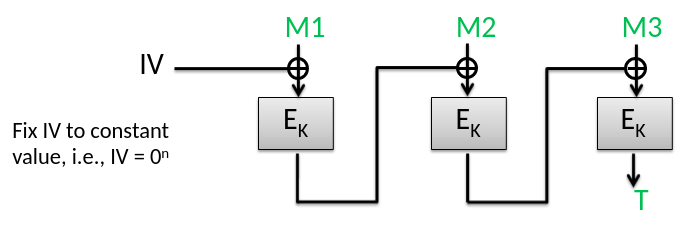
\includegraphics[width=0.5\textwidth]{notes/cbc-mac.png}
    \caption{CBC-MAC construction.}
    \label{fig:cbc-mac}
\end{figure}

To modify the construction to be deterministic, we can set the IV to be $0^n$. The output will be the final block of the ciphertext. However, the CBC-MAC construction doesn't satisfy $\UFCMA$ security. The adversary below gets advantage 
\bnm
\AdvUFCMA{\CBC\text{-}\MAC}{\advA}=1\;.
\enm
\begin{figure}[h]
	\centering
\fpage{.20}{
	\underline{$\advA^{\Tag}$}\\[1pt]
	$T_1 \gets \TagOracle(0^n)$\\
	$M = 0^n\concat T_1$\\
	Ret $(M,T_1)$
}
\end{figure}

However, we give a modified construction, Encrypted CBC-MAC (ECBC-MAC), that uses the same block cipher, $\E$, with a different key $K_2$ to encrypt the final output of the CBC-MAC. \scribenote{give either pseudocode or diagram of the construction.} We will prove that for any function $H$ that is an  $\epsilon$-almost universal (AU) hash function, the ECBC-MAC construction is a good variable input length $\PRF$. 

First, we define what it means to be an $\epsilon$-almost universal (AU) hash function.

A keyed function $H\Colon\bits^k\times\msgspace\rightarrow\bits^n$ is
an $\epsilon$-almost universal (AU) hash function  if for all $M,M'\in\msgspace$, $M \ne M'$
\bnm
  \Prob{H_K(M) = H_K(M')} \le \epsilon
\enm
where the probability is over random choice of $K$.

A computational almost universal (\cAU) hash function is a function for which all polynomial-time bounded $\cAU_H$ adversaries $\advA$ have small $\cAU_H$ advantage.
\begin{figure}[h]
\centering
\fpage{.20}{
\underline{$\cAU_H^\advA$}\\[1pt]
$M,M' \getsr \advA$\\
$K \getsr \bits^k$\\
If $M = M'$ then Ret $\false$\\
Ret $H_K(M) = H_K(M')$
}
\end{figure}

We define the advantage of a $\cAU_H$ adversary $\advA$ as
\bnm
  \AdvcAU{H}{\advA} = \Prob{\cAU^\advA_H\Rightarrow\true}\;.
\enm

\begin{figure}[h]
	\centering
	\fpage{.20}{
		\underline{$V(K,M)$}\\[1pt]
		$K_1,K_2\gets K$\\
		Ret $F(K_1, H(K_2,M))$\\
	}
\end{figure}
\begin{theorem} \label{thm:cau-vil-prf}
Let $F\Colon\bits^{k_1}\times \bits^n\rightarrow \bits^n$ be a fixed input length PRF, and let $H\Colon \bits^{k_2}\times \msgspace\rightarrow \bits^n$ be a $\cAU$ hash function. Let $V\Colon \bits^{k_1+k_2}\times \msgspace \rightarrow \bits^n$ be the variable input length PRF constructed using $F$ and $H$ as described above. Then, for any $\PRF_V$ adversary $\advA$ making $q$ queries, we can construct a $\cAU_H$ adversary $\advB$ and $\PRF_F$ adversary $\advC$ such that 
\bnm
	\AdvPRF{V}{\advA} \le \AdvcAU{H}{\advB} + \AdvPRF{F}{\advC}\;.
\enm
\scribenote{Above is a tentative theorem statement. Will fix once I write a proof.}
\end{theorem}

We show that if $E$ is a good PRF, then the CBC-MAC construction is computational almost universal.
\begin{theorem}
Let $E\Colon\bits^k\times\bits^n\rightarrow\bits^n$ and $H$ be the CBC-MAC. 
Then for any $\cAU_H$-adversary $\advA$ outputting messages of length at most
$\sigma$ blocks, for $\sigma\leq 2^n/4$, we give a $\PRF_E$-adversary $\advB$
such that
\bnm
  \AdvcAU{H}{\advA} \le \AdvPRF{E}{\advB} + \frac{\sigma^2}{2^n} \;.
\enm
Adversary $\advB$ runs in time that of $\advA$ and makes at most $2\sigma$
queries.
\label{thm:cau-cbcmac}
\end{theorem}
\begin{figure}
\centering
\fpage{.2}{
	\underline{$\G0$}\\[1pt]
	$M,M' \getsr \advA$\\
	$K \getsr \bits^k$\\
	If $M = M'$ then Ret $\false$\\
	$T \gets 0^n\semi T'\gets 0^n$ \\
	For $i=1$ to $m$ do \\
	\myInd $T\gets H_K(T\xor M[i])$\\
	For $j=1$ to $m'$ do \\
	\myInd $T'\gets H_K(T'\xor M'[j])$\\
	If $T=T'$ then Ret 1\\
	Ret $T=T'$
}
\fpage{.2}{
	\underline{$\G1$}\\[1pt]
	$M,M' \getsr \advA$\\
	If $M = M'$ then Ret $\false$\\
	$T \gets 0^n\semi T'\gets 0^n$ \\
	For $i=1$ to $m$ do \\
	\myInd $T\gets \Horacle(T\xor M[i])$\\
	For $j=1$ to $m'$ do \\
	\myInd $T'\gets \Horacle(T'\xor M'[j])$\\
	Ret $T=T'$\medskip
	
	\underline{$\Horacle(M)$}\\[1pt]
	If $T[M] = \bot$ then \\
	\myInd $T[M]\getsr \bits^n$\\
	Ret $T[M]$
}
\fpage{.22}{
	\underline{$\advB^{\Fn}$}\\[1pt]
	$M,M' \getsr \advA$\\
	If $M=M'$ then Ret 0 \\
	$T \gets 0^n\semi T'\gets 0^n$ \\
	For $i=1$ to $m$ do \\
	\myInd $T\gets \Fn(T\xor M[i])$\\
	For $j=1$ to $m'$ do \\
	\myInd $T'\gets \Fn(T'\xor M'[j])$\\
	If $T=T'$ then Ret 1\\
	Else Ret 0
}
\caption{Games and adversary for proof of Theorem~\ref{thm:cau-cbcmac}.}
\label{fig:games-cau-cbcmac}
\end{figure}

\begin{proof}
	We refer to the games and adversary in Figure~\ref{fig:games-cau-cbcmac}. Let $m$ and $m'$ respectively be the number of blocks in messages $M$ and $M'$ outputted by the $\cAU$ adversary $\advA$. 
	
	The games just explicitly describes the CBC-MAC construction within the $\cAU$ game, so 
	\bnm
	\AdvcAU{H}{\advA}=\Prob{\G0}\;.
	\enm
	Adversary $\advA$ wins in $\G1$ if there is a collision in either the inputs or the outputs of the random oracle that results in $T$ being equal to $T'$. A detailed analysis of this can be found in~\cite{black2000cbc}, and it turns out that we can bound this probability by 
	\bnm
	\Prob{\G1}\leq \frac{\sigma^2}{2^n}\;.
	\enm
	By examination, we can see that 
	\bnm
	\Prob{\PRF1_F^\advB\Rightarrow 1}=\Prob{\G0}
	\enm
	and
	\bnm
	\Prob{\PRF0_F^\advB\Rightarrow 1}=\Prob{\G1}\;.
	\enm
	Combining these, we see that 
	\begin{align*}
	\Prob{\G0}&=(\Prob{\G0}-\Prob{\G1}) + \Prob{\G1}\\
	\AdvcAU{H}{\advA}&\leq \AdvPRF{E}{\advB} + \frac{\sigma^2}{2^n}
	\end{align*}
\end{proof}

\section*{Exercises}
\begin{enumerate}[label=\textbf{Exercise \thesection.\arabic*}, wide=0pt]
	\item Prove Theorem~\ref{thm:sufcma-ufcma}. \label{exercise:sufcma-ufcma}
	\item Show that if a message authentication scheme $\MA$ is a $\MAC$, then $\UFCMA_\MA$ security is equivalent to $\SUFCMA_\MA$ security. \label{exercise:mac-sufcma-ufcma}
	\item Prove Theorem~\ref{thm:cau-vil-prf}.
\end{enumerate}
\newpage
\input{genericcomp}
\newpage
\input{advanced-ae}
\newpage
\input{aepractice}
\newpage
\input{hashfunctions}
\newpage
\input{hashfunctions2}
\input{hash/all}
\newpage
\input{hashfunctions3}
\newpage
\input{pke}
\newpage
\input{pke2}
\newpage
\input{ecc/ecc_main}
\newpage
%%%%%%%%%%%%%%%%%%%%%%%%%%%%%%%%%%%%%%%%%%%%%%%%%%%%%%%%%%%%%%%%%%%%%%%%%%%%%%%%
\section{Public Key Encryption under Chosen-Ciphertext Attacks}
\label{sec:pke}

In Chapter 19, we've laid the foundations for public key cryptography. We've also talked about RSA, one of the most widely used public key encryption schemes and its IND-CPA security. In this chapter we will see that CPA security alone will fail to capture all possible adversaries in the case of asymmetric cryptographic schemes. In this chapter we will look at some attacks on RSA and introduce the notion of Chosen-Ciphertext (CCA) security for public key encryption schemes namely RSA and ElGamal.  
We will end by introducing a more secure variant of RSA with padding namely OAEP (Optimal Asymmetric Encryption Padding). 

\subsection{Chosen-Plaintext (CPA) security}
In Chapter 10, we've looked at the notion of indistinguishability for plaintext security (IND-CPA).  
Recall that under IND-CPA the attacker has the ability to sample 2 distinct plaintext messages to be encrypted and receives one of the back encrypted. If the attacker is able to guess with a high probability (significantly higher than \( \frac{1}{2} \)) which plaintext was encrypted, he wins the IND-CPA game. This works in the case of public key encryption by modeling a encryption oracle on the public key (\(pk\)) since its always public knowledge. 

\indent The traditional goal of IND-CPA security is indistinguishability of the plaintext from its corresponding ciphertext. Thus it is sufficient to consider only adversaries that make queries to the encryption oracle. \newline
 
% IND-CPA game
\begin{center}
\fpage{.25}{
\underline{$\INDCPA^\advA_{\SE}$}\\[1pt]
$K \getsr \kg$\\
$b \getsr \bits$\\
$b' \getsr \advA^{\EncOracle}$\\
Ret $b = b'$\medskip

\underline{$\EncOracle(M_0,M_1)$}\\
If $|M_0| \ne |M_1|$ then\\
\myInd Ret $\bot$\\
$C \getsr \enc_K(M_b)$\\
Ret $C$
}
\end{center}

\indent The goal of IND-CPA security is to ensure that an attacker who sees the ciphertext gains little (to no) information when compared with an attacker who doesn't see the ciphertext. In other words, if a public key encryption scheme is IND-CPA secure then the scheme itself must be randomized. This makes sense intuitively as the scheme can trivially be broken under IND-CPA if a plaintext always deterministically encrypts to the same value under the same public key. In the last section we will look at ways to add padding to the RSA scheme to randomize the ciphertexts generated.

\indent In the following sections we will look at some example attacks on TLS and the QQ-browser to see why the IND-CPA is insufficient for security in practice for public key encryption schemes.

\subsection{TLS}
TLS is a cryptographic protocol that aims to provide secure communication to applications communicating through an insecure network. By secure communication we mean encryption of the data  being sent, authentication of the sender and integrity (being able to detect messages that have been tampered with). \newline
\indent A secure TLS connection is initially established using a set of messages exchanged between the two end points called a TLS handshake. \newline

% Note to self change this diagram to show the TLS protocol on the slides. 
% Define box and box title style
\tikzstyle{mybox} = [draw=black, very thick, rectangle, inner sep=6pt, inner ysep=10pt]
\tikzstyle{fancytitle} =[draw=black, fill=white, rectangle, very thick,  inner sep=2pt, inner ysep=5pt ]
\tikzstyle{line} = [draw, -latex']
% tha actual picture
\begin{figure} [H]
\centering
\begin{tikzpicture}
% the client box
\node [mybox] (box1){%
    %\begin{minipage}{0.30\textwidth}
    	%\begin{align*}
	\begin{tabular}{c}
		$: cHello := \{cRandom \leftarrow_{R} \{0,1\}^\lambda\}$ \\
		\\
		\\
		$: assert(verfiy(SSLCert));$ \\
		$: pms \leftarrow_{R} \{0,1\}^\lambda\ $\\
		$: msg :=  \{ E_{pk}(pms) \}$ \\
		$: cfin := \{sessionKey(cRand, sRand, pms)\}$ \\
		\\
	\end{tabular}
	%\end{align*}
    %\end{minipage}
};
\node[fancytitle, right=10pt] at (box1.north west) {Client};

\node [mybox, right=1.5cm of box1.east] (box2){%
    %\begin{minipage}{0.30\textwidth}
    	\begin{tabular}{c}
		\\
		$: sRand  \leftarrow_{R} \{0,1\}^\lambda$  \\
		$: sHello := \{SSLCert, pk, sRandom\} $  \\
		\\
		\\
		$: pms := D_{sk}(msg)$ \\
		$: sfin := \{sessionKey(cRand, sRand, pms)\}$ \\
		\\
	\end{tabular}
    %\end{minipage}
};
\node[fancytitle, right=10pt] at (box2.north west) {Server};

\draw [->] ([yshift=1.45cm]box1.east) -- ([yshift=1.25cm]box2.west) [text width=1cm, above] node {cHello};

\draw [->] ([yshift=0.5cm]box2.west) --  ([yshift=0.3cm]box1.east)  [text width=1cm, above] node {sHello};

\draw [->] ([yshift=-1.25cm]box1.east) -- ([yshift=-1.50cm]box2.west) [text width=1cm, above] node {msg};

\draw [->] ([yshift=-1.70cm]box1.east) -- ([yshift=-2.0cm]box2.west) [text width=1cm, above] node {cfin};

\draw [->] ([yshift=-2.2cm]box2.west) --  ([yshift=-2.5cm]box1.east)  [text width=1cm, above] node {sfin};

\end{tikzpicture}
\caption{Generic TLS Handshake protocol} \label{fig:TLS}
\end{figure}

% cite the generic tls handshake protocol
\indent In figure ~\ref{fig:TLS} we can see that the entire TLS handshake protocol hinges on both the client and server computing the same sessionKey. Since both the clientRandom and serverRandom are unencrypted, the only thing that keeps the session key secret is the premaster key sent from the client encrypted using the public key in step 3 (The 3rd in the round of messages sent by the client). And in the generic TLS RSA based protocol, the server behaves differently based on whether or not the encrypted premaster secret is valid or not. We will later see how an attacker can use this information to launch a man in the middle attack.

\subsubsection{A simpler example using Tencent's QQ-Browser}

%cite 
\indent In 2018, \cite{QQAttack} evaluated the security of the popular QQ browser. They found that QQ's use of textbook RSA (a generic RSA implementation from a textbook without any padding) left it vulnerable to an attack that would allow for any session to be broken by sending at most 128 separate queries to the QQ servers.\newline

\begin{figure} [H]
\centering
\begin{tikzpicture}

\node [mybox] (box1){%
	\begin{minipage}{0.40\textwidth}
	\begin{itemize}
		\item client generates a 128-bit\\ 
		AES session key using a \\
		pseudorandom generator\\
		\item client encrypts AES key with\\ 
		textbook RSA, and the WUP\\
		request in ECB mode using \\
		the session key\\
	\end{itemize}
	\end{minipage}
};
\node[fancytitle, right=10pt] at (box1.north west) {Client};

\node [mybox, right=1cm of box1.east] (box2){%
	\begin{minipage}{0.40\textwidth}
	\begin{itemize}
		 \item The server decrypts the RSA-encrypted AES key itreceived from the client using its private key, thenchooses the least significant 128 bits of the plaintextto be the AES session key.\\
		 \item The server decrypts the WUP request using the AESsession key. If the WUP request was valid,  it sends a  response  using  the decrypted  AES Session key\\
	\end{itemize}
	\end{minipage}
};
\node[fancytitle, right=10pt] at (box2.north west) {Server};

\draw [->] ([yshift=-1.50cm]box1.east) -- ([yshift=2.0cm]box2.west) [text width=1cm, above] node {"WUP"};

\draw [->] ([yshift=-1.8cm]box2.west) --  ([yshift=-1.8cm]box1.east)  [text width=1cm, above] node {"Valid"};

\end{tikzpicture}
\caption{QQ Server's WUP Request protocol} \label{fig:QQWUPReq}
\end{figure}

\indent Given above is a brief overview of how RSA is used in the QQ-Browser as part of its "WUP" Requests. Note that they don't use any form of padding to their RSA requests, and only use the last 128 bits of the decryption to be the session key and ignore everything else. We will exploit these properties to see if we can force the server to reveal some information about the key. \newline

\indent Let $ C \equiv k^e ( \bmod n )  $  be the be the RSA (with $pk = (n,e)$)  encrypted message being sent as part of the "WUP" Request for AES key $ k $. Now look at the following transformation. \newline
Let $k_b = k2^b$ i.e simply k left shifted by b bits. (Assuming we only take the 128 least significant bits of $k_b$)
\begin{align*}
C(2^{be} \bmod n) \bmod n \equiv (k^e \bmod n) (2^{be} \bmod n) \bmod n \\
					  \equiv (k^e2^{be}) \bmod n\\
					  \equiv (k2^b)^e \bmod n\\
					  \equiv C_b
\end{align*}

From the transformation above, we can see that any given ciphertext $C$ can be changed by appending $2^{be} mod n$ to it. By this, we can make it seem like $k_b$ was the key sent by the client.\newline
\indent Using the transformation from above, let us assume that an attacker that sends $C_{127}$ the encryption of $k_{127}$ (all but the highest bit zeroed out) to the server. Here the highest bit of $k_{127}$ is the lowest bit of $k$. The attacker guesses the that bit to be 0 initially and sends a corresponding EBC WUP request  with the assumed key. If the server responds to it, then the guess was correct, otherwise the attacker knows that bit to be 1. \newline
\indent Using the method above, the attacker can decrypt all bits of the key using at most 126 more queries.\newline  
\indent The other vulnerabilities found by the \cite{QQAttack} paper include:
\begin{itemize}
	\item The ability to index all the users on the site by IMEI  (International Mobile Equipment Identifier) and decrypt private information sent by them to the servers. These set of attacks were enabled by the following properties of their encryption scheme:
	\begin{itemize}
		\item poor pseudorandom number generation. (They used System.currentTimeMillis() which returns the current time in milliseconds since the last Unix epoch)
		\item Use of hard-coded symmetric keys
		\item Earlier version of RSA which used a 128 bit modulus
	\end{itemize}
	\item A man in the middle attacker could in the worst cases take control of a user device while updating the QQ service. More information about the specific attacks of this category can be found in section 5 of \cite{QQAttack}. 
\end{itemize}

\subsection{Bleichenbacher Attack}
The QQ browser attack was very simple because the form of RSA in that example had no padding associated with it. Let's look at a more generalized version of the attack on ciphertexts with the $PKCS \#1$ RSA scheme.
\subsubsection*{PKCS $\#1$ RSA Encryption} 
\begin{center}
\hfpagess{.30}{.30}{
\underline{$enc((N,e), M)$}\\[1pt]
psize $ \leftarrow |N| - |M| - 3$ \\
pad $ \leftarrow_R \{0,1\}^{psize}$ \\
X $ \leftarrow$ 00 $\Vert$ 02 $\Vert$ pad $\Vert$ 00 $\Vert$ M \\
Ret $X^e \bmod n$
}{
\underline{$dec((N,d), C)$}\\[1pt]
X $\leftarrow C^d \bmod n$ \\
aa $\Vert$ bb $\Vert$ w = X \\ 
if aa $\neq$ 0 or bb $\neq$ 02 or w $\eq$ 0 then\\
    \myInd Ret Err \\
pad $\Vert$ 00 $\Vert$ M = w \\
Ret M 
} \newline
\end{center}

\indent Given above is the basic general PKCS $\#1$ RSA scheme. As seen, it is simply a padded form of RSA. Let's call the ciphertexts whose decryptions conform to this format as PKCS conforming messages. For reference, the format is represented below in \cite{fig:PKCS}.

\begin{figure} [H]
\centering
\begin{tikzpicture}

\node (rect1) [draw,thick,minimum width=1cm,minimum height=1cm] { $00$};

\node (rect2) [draw,thick,minimum width=1cm,minimum height=1cm, right = 0cm of rect1] { $02$};

\node (rect3) [draw,thick,minimum width=3cm,minimum height=1cm, right = 0cm of rect2] { $pad$};

\node (rect4) [draw,thick,minimum width=1cm,minimum height=1cm, right = 0cm of rect3] { $00$};

\node (rect5) [draw,thick,minimum width=3cm,minimum height=1cm, right = 0cm of rect4] { $M$};

\end{tikzpicture}
\caption{PCKS Conforming messages} \label{fig:PKCS}
\end{figure}

\subsection*{The Bleichenbacher Attack}
\indent A generalized attack similar to the QQ-browser attack was suggested by Bleichenbacher in \cite{BleichRSA} for PCKS $\# 1$. In the QQ-browser attack it was very simple to transform the cipher texts since there was no padding. \newline

Let's assume for a message $M$ and RSA scheme $(pk = (n,e), sk)$. For some $s$ we want the following property. 
\begin{align*}
 C \equiv M^e ( \bmod n ) \\
 C' \equiv Cs^e \bmod n \equiv (Ms)^e \bmod n 
\end{align*}

\indent As before, for any ciphertext $C$ and $s$, the server would decrypt $Ms$ instead of $M$. But in the case of PKCS, we need to ensure that the value decrypted by the server $Ms$ is PKCS conforming. (Look at the decryption function above and note that the decrypted message is checked to see if its format is PCKS conforming) \newline

\indent For guessing the right s for the result to be PKCS compliant, the attacker makes use of a padding oracle. Given a ciphertext c, the oracle returns whether or not it is PCKS compliant. Luckily, we can estimate some bounds on the s to avoid brute forcing through all the combinations. \newline

Let n be k bytes. Note that the decryption function of RSA has a $\bmod n$ in the end. So the largest 
value decrypted is the largest number of k bytes. 

Let some $ B = 2^{8*(k-2)}$. Recall that the first two bytes of PCKS conforming messages are set, that leaves us the combinations starting from from 2B.

\begin{figure} [H]
\centering
\begin{tikzpicture}

\node (rect1) [draw,thick,minimum width=1cm,minimum height=1cm] { $00$};

\node (rect2) [draw,thick,minimum width=1cm,minimum height=1cm, right = 0cm of rect1] { $01$};

\node (rect3) [draw,thick,minimum width=7cm,minimum height=1cm, right = 0cm of rect2] { $..(k-2)$ bytes$...$};

\node (rect4) [draw,thick,minimum width=1cm,minimum height=1cm, below= of rect1] { $00$};

\node (rect5) [draw,thick,minimum width=1cm,minimum height=1cm, right = 0cm of rect4] { $11$};

\node (rect6) [draw,thick,minimum width=7cm,minimum height=1cm, right = 0cm of rect5] { $..(k-2)$ bytes $...$};


The concrete mathematical bounds for PKCS conforming cipher texts are given below in terms of the parameters of the rsa scheme $n$ and some random $s$ following the property from above. 
\end{tikzpicture}
\caption{Bounds on PCKS Conforming messages} \label{fig:PKCS1}
\end{figure}

\begin{align*}
	2B \leq Ms \bmod n < 3B \\
	\implies r \in \mathbb{Z}, (ms - r*n) \in [2B, 3B) \\
	\implies \frac{2B+rn}{s} \leq m < \frac{3B+rn}{s}
\end{align*}

The attack is very similar to the QQ browser attack after identifying the PCKS conforming set of ciphertexts. For a detailed look at the specific attack see \cite{BleichRSA}.

\subsection{Chosen-Ciphertext (CCA) security}
\indent It is clear from the attacks discussed in the previous sections that IND-CPA security is insufficient to capture the security of public key encryption. Here, we introduce the notion of chosen ciphertext security for public key cryptography. \newline

\indent Let us reconsider the notions of CCA security from symmetric cryptography. First of them is the notion of left-or-right indistinguishability. For $\LORCCA$ security (the games are given below for reference), recall that the challenge involves the adversary making queries of form $(M_0, M_1)$ (two equal length messages) to a left-or-right oracle. In the case of chiphertext attacks, the adversary is given access to the decryption oracle as well. But queries against it are not allowed (since the game can be won by default). Therefore, $\LORCCA$ is not a useful security notion for public key encryption since the adversary can never learn anything about the challenge from decryptions. \newline

\begin{center}
\hfpagess{.15}{.15}{
\underline{$\LORCCA1^\advA_{\SE}$}\\[1pt]
$(\pk,\sk) \getsr \kg$\\
$b' \getsr \advA^{\EncOracle,\DecOracle}(\pk)$\\
Ret $b'$\medskip

\underline{$\EncOracle(M_0,M_1)$}\\
$C \getsr \enc(\pk,M_1)$\\
$\calC \gets \calC \cup \{C\}$\\
Ret $C$\medskip

\underline{$\DecOracle(C)$}\\
If $C \in \calC$ then \\
\myInd Ret $\bot$\\
Ret $\dec(\sk,C)$
}{
\underline{$\LORCCA0^\advA_{\SE}$}\\[1pt]
$(\pk,\sk) \getsr \kg$\\
$b' \getsr \advA^{\EncOracle,\DecOracle}(\pk)$\\
Ret $b'$\medskip

\underline{$\EncOracle(M_0,M_1)$}\\
$C \getsr \enc(\pk,M_0)$\\
$\calC \gets \calC \cup \{C\}$\\
Ret $C$\medskip

\underline{$\DecOracle(C)$}\\
Ret $\bot$
}
\end{center}

\subsubsection*{$\INDCCA$ security}
Now we look at the notion of $\INDCCA$ security for public key cryptography. In this game, the challenger generates a public key encryption scheme $(pk, sk)$ and publishes the public key $pk$ to the adversary. The adversary has the ability to encrypt anything any number of times (since he has the public key). and can make calls to the decryption oracle on arbitrary ciphertexts. The adversary finally submits two plain texts to the challenger and receives one of them back encrypted with the public key (this is the challenge ciphertext). Finally the adversary has to guess the plain text that was encrypted. \newline
 
 \indent It is easy to see that the attacks described in the previous subsections are very similar to the game described here and they are both $\INDCCA2$ attacks. $\INDCCA1$ and $\INDCCA2$ differ in the sense that, the adversary can only query the decryption oracle once in $\INDCCA1$ and an arbitrary number of times in $\INDCCA2$ (except the challenge ciphertext in both cases).

\begin{center}
\fpage{.20}{
		\underline{$\INDCCA_\AEnc^\advA$}\\
    $(\pk,\sk) \getsr \kg$\\
    $b \getsr \bits$\\
    $b' \getsr \advA^{\EncOracle,\DecOracle}(\pk)$\\
		Ret $(b'=b)$\medskip

    \underline{$\EncOracle(M_0,M_1)$}\\
    If $|M_0| \ne |M_1|$ then\\
    \myInd Ret $\bot$\\
    $C \getsr \enc(\pk,M_b)$\\
    $\calC \gets \calC \cup \{C\}$\\
    Ret $C$\medskip

    \underline{$\DecOracle(C)$}\\
    If $C \in \calC$ then Ret $\bot$\\
    $M \getsr \dec(\sk,C)$\\
    Ret $M$
	}
\end{center}

\begin{align*}
  \AdvINDCCA{\AEnc}{\advA} &= 2\cdotsm\Prob{\INDCCA_\AEnc^\advA\Rightarrow\true} - 1
%        &= \left|\Prob{\INDCCA1_\AEnc^\advA\Rightarrow\true} - \Prob{\INDCCA0_\AEnc^\advA\Rightarrow\false}\right|
\end{align*}

\subsubsection*{ElGamal CCA security}

Let's recall the ElGamal encryption scheme from chapter 21. For reference, the encryption scheme is given below. 

\begin{figure}[H]
	\center
	\hfpages{.2}{
		\underline{$\enc(X,M)$:}\\
		$y \getsr \Z_{|\group|}$ \\
		$C_1 \gets g^y$\\
		$K \gets H(g^y || X^y)$\\
		$C_2 \gets encr_s(K, M)$\\
		Return $(C_1,C_2)$
	}{
		\underline{$\dec(x,(C_1,C_2))$:}\\
		$K \gets H(C_1 || C_{1}^{x})$\\
		$M \gets dec_s(K,C_2)$\\
		Return $M$
	}
	\caption{The ElGamal encryption scheme.}
	\label{fig:elgamal}
\end{figure}

For a generic ElGamal scheme with public key $pk$, $(c_1,c_2)$ is the cipher text that is sent to the decryption scheme. For $x \in Z_{|G|}$ where $G$ is a cyclic group with generator g, $pk = X = g^x$ and $sk = x$. 

\begin{center}
\begin{align*}
	pk = (G, q, g, h) \\
	y \leftarrow_{R} \{1, .., q-1\} \\
	(c_1, c_2) = (g^{y}, mg^{xy}) \\
	c_2.(c_{1}^{sk})^{-1} = m.g^{xy}.((g^{xy})^{-1}) = m \\
	E_{\text{elgamal}}(t) = (g^{y}, t.g^{xy}) \\
	E_{\text{elgamal}}(m).E_{\text{elgamal}}(m') = E_{\text{elgamal}}(mm')
\end{align*} 
\end{center}
\indent It is easy to see that the secrecy of message in this case hinges on being able to keep the shared secret $g^{xy}$ confidential. For a more detailed look at elGamal look at Chapter 20 of the notes. \newline

\indent From the results above, we can also see that the elGamal encryption scheme is visibly homomorphic in nature (i.e padding the message result in the decryption of modified seemingly valid message at the server), that should theoretically make it vulnerable to $\INDCCA$ attacks. But here we will reply on computational hardness of the cyclic group, to provide security against ciphertext attacks.

\begin{center}
\fpage{.20}{
\underline{$\ICDH_{G,h}^{\beta}$}\\
$x,y \getsr \Z_{|\group|}$\\
$Z' \getsr \beta^\DDHoracle(g,g^x,g^y)$\\
Ret $(Z=g^{xy})$\medskip

\underline{$\DDHoracle(\hat{Y},\hat{Z})$}\\
If $\hat{Y} = \hat{Z}$ then\\
\myInd Ret $1$\\
Ret $0$
}
\end{center}

We've previously seen the assumption of CDH (computational diffie-hellman) which makes it computationally intractable to compute the shared secret of the scheme. i.e $g^{ab}, a,b \in \{1, ..., q-1\}$. The CDH assumption is enough for IND-CPA security since, given a ciphertext $C_1,C_2$, the adversary cannot compute the shared secret to correctly guess the plaintext message from $C_2$ .\newline

\indent But CDH is not enough for IND-CCA security. As seen in the previous CCA attacks, the attacker is now able to make queries to the decryption oracle and the homomorphic nature of the ciphertexts in ElGamal is also problematic (Since the adversary can modify a given ciphertext into another valid one without having to compute the shared secret). So we'll need to add another assumption to CDH to guarantee CCA security. The new scheme is given below. \newline

\indent The Strong or interactive Computational Diffie-Hellman problem has two assumptions:
\begin{itemize}
\item CDH (Computational Diffie-Hellman) given access to a DDH oracle: This is the same CDH assumption from before.
\item Interactive assumption (or pairings): More information about this can be found in \cite{icdh}
\end{itemize}

There have been no other known attacks on ElGamal other than solving for CDH. So ElGamal is $\INDCCA$ secure given that the ICDH assumption holds.


\subsection{RSA-OAEP (Optimal Asymmetric Encryption Padding)}
In the sections about Bleichenbacher's attack and the QQ Browser attack, we've seen that both padded PKCS $\# 1$ and unpadded RSA are IND-CCA insecure. RSA-OAEP is a padded RSA encryption scheme suggested by Bellare and Rogaway in \cite{oaep}. OAEP uses a Feistel network with radom oracles to create optimal padding before RSA encryption. 

\subsection{Exercises}
\begin{itemize}
\item {Exercise 1} Give an example for a $pk,sk$ ElGamal scheme such that it is not CCA secure.
\item {Exercise 2} Show that RSA without padding is not CCA secure.
\item {Exercise 3} Differentiate between the padding in PKCS $\# 1$ and OAEP RSA Encryption shcemes. Also explain why OAEP is resistant to the Bleichenbacher's attack.
\end{itemize}




\newpage
%%%%%%%%%%%%%%%%%%%%%%%%%%%%%%%%%%%%%%%%%%%%%%%%%%%%%%%%%%%%%%%%%%%%%%%%%%%%%%%%
\section{Digital Signatures}
\label{sec:pke}

\subsection{Motivation}

First, we motivate the need for a new asymmetric primitive, \emph{digital signatures}, which are required to ensure message authenticity.


\begin{figure}[h]
\centering
\scalebox{0.8}{\input{digsigs/mitm_diffie_helman}}
  \caption{Illustration of a Man-in-the-Middle attack on Diffie-Hellman key exchange (left), and a solution deployed in TLS using digital signatures (right).  $\{\}$ indicates an asymmetric encryption operation under the specified public/secret keys.  MS is the final master shared secret.}
\label{fig:mitmdiffie}
\end{figure}

Consider the use of a key exchange algorithm such as Diffie-Hellman over a channel with no guarantee of authenticity, such as the Internet. Recall that Diffie-Hellman involves selection of a random group element $x, y$ from ${Z}_{|G|}$ by a client and server respectively, then exchanging $g$ raised to each private value and exchanging these values as $X$ and $Y$, respectively.  They then raise the received values to their private exponents, computing $X^y$ and $Y^x$ as their shared secret. This works because $Y^x=g^{yx}=g^{xy}=X^y$. But note this is not effective against passive attackers: as shown in Figure~\ref{fig:mitmdiffie}, an active \emph{Man-in-the-Middle} adversary in the middle of a communication channel can simply perform independent key exchange with both sides, picking their own $x$ and $y$ values, and tampering with and decrypting messages in the middle. The malicious man in the middle can then simply reencrypt and forward all messages from the client to the server, violating any confidentiality provided by further encryptions.

Note that this problem is not limited to Diffie-Hellman based protocols; in any protocol that exchanges secrets, an active adversary can man-in-the-middle attack a session in progress.  Because there is no way to check that the received values are actually sent by the intended server, there is no way for the client to ensure the integrity of the data used to compute its secret values (in the Diffie-Hellman protocol, $Y$).

We thus motivate and explore an asymmetric variant of the message integrity constructs we have explored earlier in the notes.  Here, data will be \emph{signed} by a secret key, and can be \emph{verified} by the corresponding public key.  Assuming we have such a primitive, the Diffie-Hellman protocol can be modified as shown in the right side of Figure~\ref{fig:mitmdiffie}, taken from the deployed TLS key exchange handshake.  In this protocol, the server presents the client with a certificate CERT, that signs the server's public key with the private key of a known authority, hardcoded on a client device.  This binds the secret key $sk_s$ to the identity the user expects of the server.  This secret key is then used to sign all protocol parameters, including nonces and the pre-secret value $X$, binding these values to the identity of the server.  The final master secret is then generated with the exchanged Diffie-Hellman secrets, as well as nonce values to prevent replay attacks.

In practice, even such certificate checks may not guarantee security in the presence of implementation failures.  One example is the well known iOS ``goto fail" exploit, present in the processing of the above protocol.  The following code was present in the verification of certificates in the server key exchange:

\begin{verbatim}
if ((err = SSLFreeBuffer(&hashCtx)) != 0)
    goto fail;
...
if ((err = SSLHashSHA1.update(&hashCtx, &signedParams)) != 0)
    goto fail;
    goto fail;  /* MISTAKE! THIS LINE SHOULD NOT BE HERE */
if ((err = SSLHashSHA1.final(&hashCtx, &hashOut)) != 0)
    goto fail;

err = sslRawVerify(...);
\end{verbatim}

Note the second \texttt{goto fail} line present in the above code.  Because of C's scoping rules, and because ``if" blocks with no braces only automatically include the first line typed after them, the second mistake line was out of scope of the previous if statement.  This means it runs unconditionally, whether or not an error was encountered.  Worse still, the \texttt{fail} subsection of code expected the \texttt{err} label to be set to a non-zero value; after all, all if clauses check for and ensure this is the case.  However, because this was being called unconditionally, it would be called if even no error exists and \texttt{err} \emph{was} set to 0.  If \texttt{err} is set to 0 (should never happen in programmer expectations), the fail handler allows a connection to go through, bypassing further checks of the certificate.

So, even invalid certificates would immediately jump to fail and succeed, assuming they did not trigger the SHA1 error check or any previous error checks above the jump to fail.  Indeed this was the case, and allowed an attacker to inject false certificates into TLS exchanges with iOS devices to fool them into accepting invalid server keys.  We leave the analysis of concrete attacks an adversary could perform with this bug in their arsenal to the reader, but note that any theoretical key exchange guarantees are only as good as their implementation.

\subsection{Security Definitions}

\begin{figure}[h]
\centering
\fpage{.2}{
		\underline{$\UFCMA_\DS^\advA$}\\
    $(\pk,\sk) \getsr \kg$\\
    $(M^*,\sigma^*) \getsr \advA^\SignOracle(\pk)$\\
    If $M^* \in \calM$ then \\
    \myInd Ret $\false$\\
		Ret $\ver(\pk,M^*,\sigma^*)$\medskip

    \underline{$\SignOracle(M)$}\\
    $\calM \gets \calM \cup \{M\}$\\
    $\sigma \getsr \sign(\sk,M)$\\
    Ret $\sigma$
}
\fpage{0.35}{\scalebox{0.5}{%%%%%%%%%%%%%%%%%%%%%%%%%%%%%%%%%%%%%%%%%%%%%%%%%%%%%%%%%%%%%%%%%%%%%%%%%%%%%%%%
\section{Digital Signatures}
\label{sec:pke}

\subsection{Motivation}

First, we motivate the need for a new asymmetric primitive, \emph{digital signatures}, which are required to ensure message authenticity.


\begin{figure}[h]
\centering
\scalebox{0.8}{\input{digsigs/mitm_diffie_helman}}
  \caption{Illustration of a Man-in-the-Middle attack on Diffie-Hellman key exchange (left), and a solution deployed in TLS using digital signatures (right).  $\{\}$ indicates an asymmetric encryption operation under the specified public/secret keys.  MS is the final master shared secret.}
\label{fig:mitmdiffie}
\end{figure}

Consider the use of a key exchange algorithm such as Diffie-Hellman over a channel with no guarantee of authenticity, such as the Internet. Recall that Diffie-Hellman involves selection of a random group element $x, y$ from ${Z}_{|G|}$ by a client and server respectively, then exchanging $g$ raised to each private value and exchanging these values as $X$ and $Y$, respectively.  They then raise the received values to their private exponents, computing $X^y$ and $Y^x$ as their shared secret. This works because $Y^x=g^{yx}=g^{xy}=X^y$. But note this is not effective against passive attackers: as shown in Figure~\ref{fig:mitmdiffie}, an active \emph{Man-in-the-Middle} adversary in the middle of a communication channel can simply perform independent key exchange with both sides, picking their own $x$ and $y$ values, and tampering with and decrypting messages in the middle. The malicious man in the middle can then simply reencrypt and forward all messages from the client to the server, violating any confidentiality provided by further encryptions.

Note that this problem is not limited to Diffie-Hellman based protocols; in any protocol that exchanges secrets, an active adversary can man-in-the-middle attack a session in progress.  Because there is no way to check that the received values are actually sent by the intended server, there is no way for the client to ensure the integrity of the data used to compute its secret values (in the Diffie-Hellman protocol, $Y$).

We thus motivate and explore an asymmetric variant of the message integrity constructs we have explored earlier in the notes.  Here, data will be \emph{signed} by a secret key, and can be \emph{verified} by the corresponding public key.  Assuming we have such a primitive, the Diffie-Hellman protocol can be modified as shown in the right side of Figure~\ref{fig:mitmdiffie}, taken from the deployed TLS key exchange handshake.  In this protocol, the server presents the client with a certificate CERT, that signs the server's public key with the private key of a known authority, hardcoded on a client device.  This binds the secret key $sk_s$ to the identity the user expects of the server.  This secret key is then used to sign all protocol parameters, including nonces and the pre-secret value $X$, binding these values to the identity of the server.  The final master secret is then generated with the exchanged Diffie-Hellman secrets, as well as nonce values to prevent replay attacks.

In practice, even such certificate checks may not guarantee security in the presence of implementation failures.  One example is the well known iOS ``goto fail" exploit, present in the processing of the above protocol.  The following code was present in the verification of certificates in the server key exchange:

\begin{verbatim}
if ((err = SSLFreeBuffer(&hashCtx)) != 0)
    goto fail;
...
if ((err = SSLHashSHA1.update(&hashCtx, &signedParams)) != 0)
    goto fail;
    goto fail;  /* MISTAKE! THIS LINE SHOULD NOT BE HERE */
if ((err = SSLHashSHA1.final(&hashCtx, &hashOut)) != 0)
    goto fail;

err = sslRawVerify(...);
\end{verbatim}

Note the second \texttt{goto fail} line present in the above code.  Because of C's scoping rules, and because ``if" blocks with no braces only automatically include the first line typed after them, the second mistake line was out of scope of the previous if statement.  This means it runs unconditionally, whether or not an error was encountered.  Worse still, the \texttt{fail} subsection of code expected the \texttt{err} label to be set to a non-zero value; after all, all if clauses check for and ensure this is the case.  However, because this was being called unconditionally, it would be called if even no error exists and \texttt{err} \emph{was} set to 0.  If \texttt{err} is set to 0 (should never happen in programmer expectations), the fail handler allows a connection to go through, bypassing further checks of the certificate.

So, even invalid certificates would immediately jump to fail and succeed, assuming they did not trigger the SHA1 error check or any previous error checks above the jump to fail.  Indeed this was the case, and allowed an attacker to inject false certificates into TLS exchanges with iOS devices to fool them into accepting invalid server keys.  We leave the analysis of concrete attacks an adversary could perform with this bug in their arsenal to the reader, but note that any theoretical key exchange guarantees are only as good as their implementation.

\subsection{Security Definitions}

\begin{figure}[h]
\centering
\fpage{.2}{
		\underline{$\UFCMA_\DS^\advA$}\\
    $(\pk,\sk) \getsr \kg$\\
    $(M^*,\sigma^*) \getsr \advA^\SignOracle(\pk)$\\
    If $M^* \in \calM$ then \\
    \myInd Ret $\false$\\
		Ret $\ver(\pk,M^*,\sigma^*)$\medskip

    \underline{$\SignOracle(M)$}\\
    $\calM \gets \calM \cup \{M\}$\\
    $\sigma \getsr \sign(\sk,M)$\\
    Ret $\sigma$
}
\fpage{0.35}{\scalebox{0.5}{%%%%%%%%%%%%%%%%%%%%%%%%%%%%%%%%%%%%%%%%%%%%%%%%%%%%%%%%%%%%%%%%%%%%%%%%%%%%%%%%
\section{Digital Signatures}
\label{sec:pke}

\subsection{Motivation}

First, we motivate the need for a new asymmetric primitive, \emph{digital signatures}, which are required to ensure message authenticity.


\begin{figure}[h]
\centering
\scalebox{0.8}{\input{digsigs/mitm_diffie_helman}}
  \caption{Illustration of a Man-in-the-Middle attack on Diffie-Hellman key exchange (left), and a solution deployed in TLS using digital signatures (right).  $\{\}$ indicates an asymmetric encryption operation under the specified public/secret keys.  MS is the final master shared secret.}
\label{fig:mitmdiffie}
\end{figure}

Consider the use of a key exchange algorithm such as Diffie-Hellman over a channel with no guarantee of authenticity, such as the Internet. Recall that Diffie-Hellman involves selection of a random group element $x, y$ from ${Z}_{|G|}$ by a client and server respectively, then exchanging $g$ raised to each private value and exchanging these values as $X$ and $Y$, respectively.  They then raise the received values to their private exponents, computing $X^y$ and $Y^x$ as their shared secret. This works because $Y^x=g^{yx}=g^{xy}=X^y$. But note this is not effective against passive attackers: as shown in Figure~\ref{fig:mitmdiffie}, an active \emph{Man-in-the-Middle} adversary in the middle of a communication channel can simply perform independent key exchange with both sides, picking their own $x$ and $y$ values, and tampering with and decrypting messages in the middle. The malicious man in the middle can then simply reencrypt and forward all messages from the client to the server, violating any confidentiality provided by further encryptions.

Note that this problem is not limited to Diffie-Hellman based protocols; in any protocol that exchanges secrets, an active adversary can man-in-the-middle attack a session in progress.  Because there is no way to check that the received values are actually sent by the intended server, there is no way for the client to ensure the integrity of the data used to compute its secret values (in the Diffie-Hellman protocol, $Y$).

We thus motivate and explore an asymmetric variant of the message integrity constructs we have explored earlier in the notes.  Here, data will be \emph{signed} by a secret key, and can be \emph{verified} by the corresponding public key.  Assuming we have such a primitive, the Diffie-Hellman protocol can be modified as shown in the right side of Figure~\ref{fig:mitmdiffie}, taken from the deployed TLS key exchange handshake.  In this protocol, the server presents the client with a certificate CERT, that signs the server's public key with the private key of a known authority, hardcoded on a client device.  This binds the secret key $sk_s$ to the identity the user expects of the server.  This secret key is then used to sign all protocol parameters, including nonces and the pre-secret value $X$, binding these values to the identity of the server.  The final master secret is then generated with the exchanged Diffie-Hellman secrets, as well as nonce values to prevent replay attacks.

In practice, even such certificate checks may not guarantee security in the presence of implementation failures.  One example is the well known iOS ``goto fail" exploit, present in the processing of the above protocol.  The following code was present in the verification of certificates in the server key exchange:

\begin{verbatim}
if ((err = SSLFreeBuffer(&hashCtx)) != 0)
    goto fail;
...
if ((err = SSLHashSHA1.update(&hashCtx, &signedParams)) != 0)
    goto fail;
    goto fail;  /* MISTAKE! THIS LINE SHOULD NOT BE HERE */
if ((err = SSLHashSHA1.final(&hashCtx, &hashOut)) != 0)
    goto fail;

err = sslRawVerify(...);
\end{verbatim}

Note the second \texttt{goto fail} line present in the above code.  Because of C's scoping rules, and because ``if" blocks with no braces only automatically include the first line typed after them, the second mistake line was out of scope of the previous if statement.  This means it runs unconditionally, whether or not an error was encountered.  Worse still, the \texttt{fail} subsection of code expected the \texttt{err} label to be set to a non-zero value; after all, all if clauses check for and ensure this is the case.  However, because this was being called unconditionally, it would be called if even no error exists and \texttt{err} \emph{was} set to 0.  If \texttt{err} is set to 0 (should never happen in programmer expectations), the fail handler allows a connection to go through, bypassing further checks of the certificate.

So, even invalid certificates would immediately jump to fail and succeed, assuming they did not trigger the SHA1 error check or any previous error checks above the jump to fail.  Indeed this was the case, and allowed an attacker to inject false certificates into TLS exchanges with iOS devices to fool them into accepting invalid server keys.  We leave the analysis of concrete attacks an adversary could perform with this bug in their arsenal to the reader, but note that any theoretical key exchange guarantees are only as good as their implementation.

\subsection{Security Definitions}

\begin{figure}[h]
\centering
\fpage{.2}{
		\underline{$\UFCMA_\DS^\advA$}\\
    $(\pk,\sk) \getsr \kg$\\
    $(M^*,\sigma^*) \getsr \advA^\SignOracle(\pk)$\\
    If $M^* \in \calM$ then \\
    \myInd Ret $\false$\\
		Ret $\ver(\pk,M^*,\sigma^*)$\medskip

    \underline{$\SignOracle(M)$}\\
    $\calM \gets \calM \cup \{M\}$\\
    $\sigma \getsr \sign(\sk,M)$\\
    Ret $\sigma$
}
\fpage{0.35}{\scalebox{0.5}{\input{digsigs/digsigs}}}

\bnm
  \AdvUFCMA{\DS}{\advA} = \Prob{\UFCMA_{\DS}^\advA\Rightarrow\true}
\enm

  \caption{Our desired asymmetric signature primitive allows for message authentication using a public key.  The security game is shown to the left, with the operation of the \texttt{kg}, \texttt{sign}, and \texttt{ver} primitives shown on the right.  $\sigma$ is referred to as the signature.  The sign operation is often randomized.  }
\label{fig:digsigvisual}
\end{figure}

Figure~\ref{fig:digsigvisual} shows the UF-CMA security game and a visual representation of the operation of our desired digital signature primitives.  An encryption key consists of a key generation routing, which generates a randomized secret and public key, and a signing routine that outputs a signature for a message given the secret key.

Formally, a digital signature scheme $\DS = (\kg,\sign,\ver)$ is a triple of
algorithms. Key generation is randomized and outputs a key pair $(\pk,\sk)$,
where $\pk$ is called the public or verification key and $\sk$ is called the secret or
signing key.
Signing takes as input a secret key $\sk$ and a message $M$ and outputs a
signature, usually denoted $\sigma$.
Verification takes as input a public key $\pk$, message $M$, and signature
$\sigma$ and outputs a
bit.

The advantage of an adversary against $\UFCMA_{\DS}$ security is defined as the probability it can generate a signature accepted by \texttt{ver} that was not generated by a signing oracle to which it has access.  Unlike in the message integrity $\UFCMA$ setting, we give the adversary access to the public key, as this key is public knowledge.  This implies the adversary can also run \texttt{ver} to check the validity of signatures.

We will now take show that one strawman plaintext RSA-based digital signature scheme fails to meet $\UFCMA_{\DS}$ security, then informally argue that another RSA-based scheme that is widely used in practice, PKCS v1.5, also fails to meet $\UFCMA_{\DS}$ security; the full proof is left as an exercise to the reader.  We then complete our analysis by proving $\UFCMA_{\DS}$ security for the ``full domain hash" RSA scheme.

\subsection{Straw-Man: Plaintext RSA}


\begin{figure}[h]
\centering
\fpage{.3}{
		\underline{$\kg$}\\
		Generate RSA (sk, pk) $((N, d), (N, e))$ \\
    Ret $((N,d), (N, e))$\\ \\
		\underline{$\sign((N, d), M)$}\\
    Ret $M^d\mod N$\\ \\
		\underline{$\ver((N, e), M, \sigma)$}\\
    Ret $\sigma^e\mod N = M$
}
\fpage{.25}{
		\underline{$\advA^{\SignOracle}(\pk=(N, e))$}\\
		$M^* \getsr Z^*_N$ \\
		$R \getsr Z^*_N$ \\
		$\sigma^* \gets \Sign(R^e M^*\mod N)$ \\
		Ret $(M^*, (\sigma^* R^{-1})\mod N)$
}
\bnm
  \AdvUFCMA{\DS}{\advA^\SignOracle} = \Prob{\UFCMA_{\DS}^{\advA^\SignOracle}\Rightarrow\true} \approx 1
\enm

  \caption{The plaintext RSA operation (left) uses the same key format and general structure as RSA encryption.  The adversary for this scheme (right) breaks $\UFCMA_{\DS}$ security with advantage of approximately 1.}
\label{fig:plaintextrsa}
\end{figure}

Figure~\ref{fig:plaintextrsa} shows a natural adaptation of plaintext (textbook) RSA to digital signatures.  The sign routine raises the message $M$ to the secret exponent $d$; for verification, the signature is raised to the public exponent $e$, taking advantage of the property that $m^{ed}\mod N=m\mod N$ (also used in RSA decryption to invert the RSA permutation without revealing the secret value $d$) for correctness.

However, the given adversary breaks $\UFCMA_{\DS}$ security with advantage of approximately 1, as we now argue.  Note that $\sigma^* = (R^e M^*)^d\mod N$ (by definition of sign) $ = (R^{ed} M^{*d})\mod N = (R^{ed}\mod N) (M^{*d}\mod N) = (R\mod N) (M^{*d}\mod N)$ (by RSA permutation) $ = \sigma$.

Note that the signature that our adversary returns for $M^*$ is $(\sigma R^{-1})\mod N$.  So, by the above, this is equal to $(R^{-1} ((R\mod N) (M^{*d}\mod N))\mod N = M^{*d}\mod N$, the exact signature generated by \texttt{sign} for $M^*$ by construction.

Note that our adversary generated a valid signature for $M^*$ making a single signing oracle query to $R^e M^*$.  Because $R$ is sampled at random from $\Z^*_N$, the probability that the adversary has queried the oracle on $M^* = $Pr$[R^e M^*=M^*] = \frac{1}{|\Z^*_N|}$.  Hence, our $A^\Sign$ wins the UF-CMA game with advantage $1 - \frac{1}{|\Z^*_N|} \approx 1$ for sufficiently large $N$.

Note that the above argument does not depend on a random choice of $M*$, and indeed applies to any $M^*$, which could be passed into our adversary as input.  This makes our attack a \emph{universal} forgery against RSA; that is, $\forall$ messages $M^*$, our adversary can provide a forged signature $\sigma^*$ without querying the real signature routine on $M^*$ with non-negligible advantage.  A weaker kind of forgery, \emph{existential forgery}, exists in a scheme if $\exists M^*$ such that an adversary can generate a forged signature $\sigma^*$ without querying the real signature routine on $M^*$ with non-negligible advantage.  Note that the existence of a universal forgery attack implies an existential forgery attack but not vice-versa, making universal forgery a stronger form of forgery than existential forgery.

\subsection{Insecurity in Practice: PKCS\#1 v1.5}


\begin{figure}[h]
\centering
\fpage{.25}{
		\underline{$\sign((N, d), M)$}\\
		$Y = 00 || 01 || FF^p || 00 || H(M)$
    Ret $Y^d\mod N$

}
\fpage{.45}{
		\underline{$\ver((N, e), M)$}\\
		$Y = \sigma^e\mod N$ \\
		Let $aa || bb || cc || dd || h = Y$ \\
		If $(aa \neq 00)$ or $(bb \neq 01)$ or $(cc \neq FF^p)$ or $(dd \neq 00)$: \\
		\myInd Ret error // Vulnerable to padding oracle attacks \\
		Ret $H(m) = h$

}

  \caption{The PKCS\#1 v1.5 signing construction uses a hash function to prevent the predictable algebraic manipulation of a message to which our plain-text straw man scheme is vulnerable.  In this case, let $N$ have $n$ bytes and the the output of $H$ have $m$ bytes; then, $p=n - m - 3$, providing a total output length of $n$ bytes.}
\label{fig:pkcs15sign}
\end{figure}



Figure~\ref{fig:pkcs15sign} shows a construction deployed in practice for RSA-based signing, PKCSv1.5.  In this scheme, the general structure of our plaintext RSA signing scheme is preserved, but the message is padded with additional data, and a hash of the message is included for exponentiation with the private RSA exponent rather than the full message.  This hash appears to protect against the form of attack we have seen above.

Intuitively, this makes malleability attacks like the form we have seen above more difficult; even if an adversary could use the techniques we show to generate a valid $\sigma$ for some $x=H(M')$ given a signature $\sigma^*$ for $H(M^*)$, they would be unlikely to generate a signature that verifies for a known message, as they would need to provide some $M'$ to a verification oracle along with $\sigma$ such that $H(M')=x$, inverting the hash function used for signing.  Use of a pre-image resistant hash function therefore poses a barrier to an adversary's forgery attempts; they can generate a signature that is valid for \emph{some} message, without the ability to produce the message for which that signature is valid.  We formalize this intuition in the proof of Full-Domain RSA that follows.

The padding in the scheme also appears to provide additional protections: If, for example, an adversary changes bits in the padding section of signed values, the mangled padding should produce an error and fail to verify, further restricting the adversary's ability to produce valid signature values for some message without querying the signing oracle.  However, as previously explored in the notes, red flags should be raised about the use of padding in a context able to generate padding-specific errors; in fact, because the padding scheme is similar to that in RSA PKCS\#1 v1.5 encryption, the same attack is usable to extract key material in our signing scheme, violating $\UFCMA_{\DS}$ security.  The proof is left as an exercise to the reader.

We now move to a formal proof of $\UFCMA_{\DS}$ security for a hash-based RSA construction that \emph{does} provide such security.  We use a full domain hash to avoid such padding leakage issues, and to simplify our reasoning about the security of the scheme.

\subsection{A Secure Scheme: Full Domain RSA}


We now introduce the full domain hash (FDH) RSA scheme, denoted $\DS$.  Figure~\ref{fig:fulldomrsa} shows the operation of this scheme, which is a natural extension of plaintext RSA that simply hashes the message before exponentiating with a secret exponent.  Note that we model the hash function as a random oracle, which masks some subtle technical issues surrounding use of a hash with RSA; because $H(M)$ needs to be raised to the $d$ (mod $N$), $H(M)$ must output an element of the RSA group that can be exponentiated in the group.  So, the hash function used depends on the choice of $d$, which complicates analysis.  We ignore these details in our consideration of the protocol, as they can be solved in practice by using a fixed output length hash that is indifferentiable from random oracles using existing hash functions, and mapping the output of the function to the relevant RSA group.

We now analyze the $\UFCMA_\DS$ security of our scheme.  We do so by reduction to RSA, showing specifically that for any adversary $A$ breaking the $\UFCMA_\DS$ of full domain RSA, we can construct an adversary $B$ for the RSA game with almost the same advantage.  Formally, let $q_h$ be the number of hash oracle queries performed by $A$ and $q_s$ be the number of signing oracle queries performed by $A$:

\begin{theorem*}
Let $\DS$ be the FDH scheme using $\RSAk$ and $\Horacle\Colon\msgspace\rightarrow\Z_N^*$ modeled as
a RO. Let $\advA$ be any $\UFCMA_\DS$-adversary making at most $q_h$ queries to
$\Horacle$ and $q_s$ queries to its signing oracle. 
Then we give an $\RSAk$-adversary $\advB$ such that
\bnm
    \AdvUFCMA{\DS}{\advA} \le (q_h + q_s + 1) \cdotsm\AdvOWF{\RSAk}{\advB}
\enm
Adversary~$\advB$ runs in time that of $\advA$ plus $\bigO(q_s+q_h)$. 
\end{theorem*}


\begin{proof}
To start we make some simplifying assumptions about $\advA$, and justify that these assumptions are without loss.

\textbf{Lemma 1} Let $A$ be any adversary that does not match our assumptions.  We will show that there exists some $A'$ such that $A'$ has the same advantage as $A$, and runs in at most $q_s+1$ additional oracle queries.  Let $M*$ be the message on which $A$ outputs a valid forgery, as in the game definition.

Our simplifications are as follows:
\begin{itemize}
	\item Whenever $A$ makes a query to $\SignOracle$ on a message $M$, it has previously made a query
$\Horacle(M)$.  If this assumption is not met, we transform $A$ to an equivalent $A'$ that queries $\Horacle(M)$ before $\Signoracle(M)$ for every query to the sign oracle, discarding the result.  Note that $A$ and $A'$ have identical output for all inputs, as our spurious oracle calls are discarded and do not affect the output subsequent calls to $\Horacle$ or $\Signoracle$ by inspection.  $A'$ runs in at most $q_s$ additional oracle queries by construction.
	\item $A$ always queries $\Horacle(M^*)$.  If not, at the end of executing $A$, $A'$ inserts and discards a synthetic query to $\Horacle(M^*)$. As in the above, spurious calls are disregarded and the advantage for $A, A'$ remains identical.  $A'$ runs in at most $1$ additional oracle query by construction.
	\item $A$ does not query $\Signoracle(M^*)$.  If instead $A$ does query $\Signoracle(M^*)$, we simply abort $A'$.  Note that if $A$ queries $\Signoracle(M^*)$, it succeeds with probability $0$, as by construction of the game $M*$ is in the set $\calM$ and has been signed by the oracle.  In this case, $A'$ fails (succeeds with probability $0$), meaning the advantage of $A'$ is exactly equal to that of $A$.  $A'$ makes one fewer oracle query than $A$ by construction.
	\item $A$ does not query $\Horacle$ or $\Signoracle$ twice on the same $M^*$.  If this is not the case, $A'$ can simply memoize all the deterministic calls to $\Horacle$ and $\Signoracle$, acting on the same oracle outputs as $A$ and thus yielding identical executions for all inputs without the need to repeat calls.  $A'$ makes fewer oracle queries than $A$ by construction.
\end{itemize}

So, we can consider only $A$ that meet our assumptions without loss of generality, as if such an $A$ exists, there exists an $A'$ that runs in at most $1+q_s$ additional $\Horacle$ oracle queries with the same advantage.  Lemma 1 holds.

\textbf{Toy example - No-message attack} Now, to build some intuition, let's first consider the case that $q_s = 0$, that is, 
we are arguing about unforgeability in a no-message attack where no legitimate signatures are produced by the signing oracle for the adversary.  Our key challenge is to construct such an adversary $B$ for RSA OWF; to do so, we must use an adversary for $\UFCMA_{\DS}$ as a black box.  Figure~\ref{fulldomaintoy} shows such an adversary, as well as the games required to prove security.  Our general proof will proceed by choosing a point $Y$ as the output of a simulated hash oracle, where $Y$ represents the point the adversary of an RSA OWF game needs to invert as a challenge.  Because our hash function is a random oracle, to recover the original signed message, our $\UFCMA_{\DS}$ adversary will need to invert the hash function on some queried point.  Specifically, they must do this on the point corresponding to the hash of $M^*$, the challenge for which they provide a valid signature; because our hash function is a random oracle, they must do this to get any information about the output of the hash function on $M^*$, required by construction to generate a valid signature (if no information about $H(M^*)$ is known, every possible output signature is equally likely by the RSA permutation's properties as a permutation).

Such an adversary can, however, query the hash oracle on multiple points, and it is not clear for which point to provide them with the OWF challenge $Y$.  
%Assume that $\advA$
%queries $\Horacle(M^*)$ where $M^*$ is the output message for its forgery. This
%is without loss. 
Our solution is to 
guess which random oracle query corresponds to the solution, and program its
output to be equal be the OWF challenge $Y$.  In more detail, we set our forgery
adversary $\advB$ to be as shown in Figure~\ref{fig:fulldomaintoy}.  Let $i^*$ be our guess for which index represents a query to $M^*$, and $i$ be the index of the next oracle query to be performed.
%Intuitively, to forge against FDH one needs to invert RSA on $\Horacle(M)$ for
%some $M$. Then we can build an inverter $\advB$ that works as follows. 

\begin{figure}
\centering
\fpage{.22}{
\underline{$\UFCMA_{\DS}$}\\
$((N,e),(N,d)) \getsr \kg$\\
$(M^*,\sigma^*) \getsr \advA^{\Horacle,\SignOracle}((N,e))$\\
If $M^* \in \calM$ then Ret $\false$\\
Ret $\left(\TabH[M^*] = (\sigma^*)^e \bmod N\right)$\medskip

\underline{$\Horacle(M)$}\\
If $\TabH[M] = \bot$ then\\
\myInd $\TabH[M] \getsr \Z_N^*$\\
Ret $\TabH[M]$\medskip

\underline{$\SignOracle(M)$}\\
$\calM \gets \calM \cup \{M\}$\\
$X \getsr \Horacle(M)$\\
Ret $X^d \bmod N$
}
\fpage{.22}{
\underline{$\G_0$ \;\;\; \fbox{$\G_1$}}\\
$((N,e),(N,d)) \getsr \kg$\\
$i^* \getsr [1,q]$\\
$i \gets 0$\\
$(M^*,\sigma^*) \getsr \advA^{\HashSim}((N,e))$\\
If $(M^* \ne M_{i^*})$ then \\
\myInd $\badtrue$\\
\myInd \fbox{Ret $\false$}\\
Ret $\left(\TabH[M^*] = (\sigma^*)^e \bmod N\right)$\medskip

\underline{$\HashSim(M)$}\\
$i \gets i+1$\\
$M_i \gets M$\\
If $i = i^*$ then\\
\myInd Ret $\TabH[M_i] \getsr \Z_N^*$\\
$\TabH[M_i] \getsr \Z_N^*$\\
Ret $\TabH[M_i]$
}
\fpage{.22}{
\underline{$\G_2$}\\
$((N,e),(N,d)) \getsr \kg$\\
$i^* \getsr [1,q]$\\
$i \gets 0$\\
$(M^*,\sigma^*) \getsr \advA^{\HashSim}((N,e))$\\
If $(M^* \ne M_{i^*})$ then \\
\myInd $\badtrue$\\
\myInd Ret $\false$\\
Ret $\left(\TabH[M^*] = (\sigma^*)^e \bmod N\right)$\medskip

\underline{$\HashSim(M)$}\\
$i \gets i+1$\\
$M_i \gets M$\\
If $i = i^*$ then\\
\myInd Ret $\TabH[M_i] \gets Y$\\
$\TabH[M_i] \getsr \Z_N^*$\\
Ret $\TabH[M_i]$
}
\fpage{.22}{
\underline{$\advB_{toy}((N,e),Y)$}\\
$(M^*,\sigma^*) \getsr \advA^{\HashSim}((N,e))$\\
Ret $\sigma^*$\medskip

\underline{$\HashSim(M)$}\\
If $i = i^*$ then\\
\myInd Ret $Y$\\
$X \getsr \Z_N^*$\\
Ret $X$
}
  \caption{Toy example of full-domain RSA hash signing with no signing queries.}
\label{fig:fulldomaintoy}
\end{figure}


Intuitively $\advB$ wins as long as $\advA$ wins and $i^*$ is the correct guess
of which hash query by $\advA$ corresponds to the winning $M^*$. (Recall that we
are assuming that $\advA$ always queries $\Horacle$ for the forgery message
$M^*$.) To analyze this, let game $\G_0$ be equal to $\UFCMA_{\DS}^\advA$ except
that it additionally includes a random choice of $i^* \getsr [1,q]$ and sets a
flag $\bad$ to true should $M^* \ne M_{i^*}$. Let
game $\G_1$ be the same as $\G_0$ except that  it chooses a random index $i^*
\getsr [1,q]$ and checks if $M^*$ is equal to the $i\thh$ random oracle
query. If not, it sets a flag $\bad$ to true and outputs $\false$, 
Otherwise it checks if $\advA$'s output is a winning forgery, outputting
$\true$ if so and $\false$ otherwise. Let $\good$ be the event that $\bad$ is
not set in game $\G_0$, and we let $\good$ be the same event for $\G_1$ (a
slight abuse of notation). Then we have that both games are
identical-until-$\bad$ and a variant of the fundamental lemma of game playing
says that:
\bnm
  \Prob{\G_0 \Rightarrow\true \land\good} = \Prob{\G_1\Rightarrow\true \land
  \good} \;.
\enm
Then using this, we have that:
\iffalse
\begin{align*}
\AdvOWF{\RSAk}{\advB_{toy}} 
%  &= \Prob{\G_0\Rightarrow\true} (1)
  &\ge \Prob{\G_0\Rightarrow\true\land\good} (2)\\
  &= \Prob{\G_1\Rightarrow\true\land\good} (3)\\
  &= \Prob{\G_1\Rightarrow\true}\cdot\Prob{\good} (4)\\
  &= \AdvUFCMA{\DS}{\advA}\cdotsm\frac{1}{q_h} (5)
\end{align*}
\fi

\begin{align*}
\AdvOWF{\RSAk}{\advB_{toy}} 
  &= \Prob{\G_2\Rightarrow\true} (1) \\
  &= \Prob{\G_1\Rightarrow\true} (2)
  \ge \Prob{\G_1\Rightarrow\true\land\good} (3)\\
  &= \Prob{\G_0\Rightarrow\true\land\good} (4)
  = \Prob{\G_0\Rightarrow\true}\cdot\Prob{\good} (5)\\
  &= \AdvUFCMA{\DS}{\advA}\cdotsm\frac{1}{q} (6)
\end{align*}


$(1)$ follows because $\G_0$ outputs \texttt{true} iff $\TabH[M^*] = (\sigma^*)^e \bmod N$.  Note that $\TabH[M^*] = Y$ (because $\G_0$ outputs false if $M_{i^*}\neq M^*$, and by construction of the hash oracle).  So, $Y=(\sigma^*)^e \bmod N$ for B's challenge in the OWF game, and $B$ outputs $(\sigma^*)$, winning the OWF game.

$(2)$ follows because $G_2, G_1$ differ only in the output of $\TabH[M^{M^*}]$ (as above, in both, either game returning true implies $M_{i^*} = M^*$).  But, in one case, a point sampled from $\calZ_N$ is returned, and in another, $Y$ is returned, which is a point sampled from $\calZ_N$ by definition of the challenge provided $B$ in the OWF game.  It is thus impossible for this difference in identically distributed random choice to affect the operation of $A$.

$(3)$ follows from basic probability, and $(4)$ follows from our variant of the fundamental lemma of game playing, above.  $(5)$ follows as the probability that the good flag is set in $G_1$ is exactly equal to the probability that $M^* = M_{i^*}$, which is by definition the probability that the $i^*$th query of $q_h$ total queries to the hash oracle has as input $M^*$.  Because $i$ is independently uniformly sampled, this probability is equal for every choice of $i$, independent of all other values. $(6)$ follows as Lemma 1 states that $M^*$ will be exactly one of the queries to the hash oracle (in this case equal to the number of total queries, $q$, as $q_s=0$), making this probability exactly equal to $\frac{1}{q}$.  Note that concretely here, $q=q_h+1$ by Lemma 1.

\textbf{Generalization of toy example to full proof.}  We now must do a generalization of the above to cases where $q_s \geq 1$, that is, our black-box $\UFCMA_\DS$ adversary makes at least one signing query.  In these cases, we face a substantive challenge: because the hash function in our full domain RSA construction is used by the signing routine, it is not the case that sign function outputs are independent of the outputs of our hash function.  We therefore cannot simply return random points for both the sign and hash function, as this breaks the structure of signatures; for example, any adversary that runs \texttt{ver} on outputs of \texttt{sign} would receive outputs of $1$ with a valid signature and hash function, and $0$ if we return random points, altering its execution and therefore output with overwhelming probability.

We therefore must program the signature oracle to return points which constitute valid signatures for points on which the hash oracle has already been queried (by Lemma 1, we can assume this is always the case).  So, as desired, we have that $\AdvOWF{\RSAk}{\advB_{toy}} \ge \AdvUFCMA{\DS}{\advA}\cdotsm\frac{1}{q}$, completing the proof.



\begin{figure}
\centering
\fpage{.30}{
\underline{$\advB((N,e),Y)$}\\
$i^* \getsr [1,q]$\\
$i \gets 0$\\
$(M^*,\sigma^*) \getsr \advA^{\HashSim,\SignSim}((N,e))$\\
If $(M^* \ne M_{i^*})$ then $X' \getsr \Z_N^*$\\
Else $X' \gets \sigma^*$\\
Ret $X'$\medskip

\underline{$\HashSim(M)$}\\
$i \gets i+1$\\
$M_i \gets M$\\
If $i = i^*$ then\\
\myInd Ret $Y$\\
$\sigma_i \getsr \Z_N^*$\\
$\TabH[M_i] \gets (\sigma_i)^e \bmod N$\\
Ret $\TabH[M_i]$\medskip

\underline{$\SignSim(M)$}\\
Let $i$ be s.t.~$M_i = M$\\
If $i = i^*$ then\\
\myInd Ret $\sigma \getsr \Z_N^*$\\
Ret $\sigma_i$
}
\fpage{.30}{
\underline{$\G_0$}\\
$((N,e),(N,d) \getsr \kg$\\
$X \getsr \Z_N^*$\\
$Y \gets X^e \bmod N$\\
$i^* \getsr [1,q]$\\
$i \gets 0$\\
$(M^*,\sigma^*) \getsr \advA^{\HashSim,\SignSim}((N,e))$\\
If $(M^* \ne M_{i^*})$ then \\
\myInd $\badtrue$\\
\myInd $X' \getsr \Z_N^*$\\
$X' \gets \sigma^*$\\
Ret $(X = X')$\medskip

\underline{$\HashSim(M)$}\\
$i \gets i+1$\\
$M_i \gets M$\\
If $i = i^*$ then\\
\myInd Ret $Y$\\
$\sigma_i \getsr \Z_N^*$\\
$\TabH[M_i] \gets (\sigma_i)^e \bmod N$\\
Ret $\TabH[M_i]$\medskip

\underline{$\SignSim(M)$}\\
Let $i$ be s.t.~$M_i = M$\\
If $i = i^*$ then\\
\myInd $\badtrue$\\
\myInd Ret $\sigma \getsr \Z_N^*$\\
Ret $\sigma_i$
}
\fpage{.30}{
\underline{$\G_1$}\\
$((N,e),(N,d) \getsr \kg$\\
$X \getsr \Z_N^*$\\
$Y \gets X^e \bmod N$\\
$i^* \getsr [1,q]$\\
$i \gets 0$\\
$(M^*,\sigma^*) \getsr \advA^{\HashSim,\SignSim}((N,e))$\\
If $(M^* \ne M_{i^*})$ then \\
\myInd $\badtrue$\\
\myInd $X' \gets \sigma^*$\\
$X' \gets \sigma^*$\\
Ret $(X = X')$\medskip

\underline{$\HashSim(M)$}\\
$i \gets i+1$\\
$M_i \gets M$\\
If $i = i^*$ then\\
\myInd Ret $Y$\\
$\sigma_i \getsr \Z_N^*$\\
$\TabH[M_i] \gets (\sigma_i)^e \bmod N$\\
Ret $\TabH[M_i]$\medskip

\underline{$\SignSim(M)$}\\
Let $i$ be s.t.~$M_i = M$\\
If $i = i^*$ then\\
\myInd $\badtrue$\\
\myInd Ret $\sigma \gets X$\\
Ret $\sigma_i$
}


\begin{align*}
  \AdvUFCMA{\DS}{\advA} &= \Prob{\G_1\Rightarrow\true}\\
      &\le \Prob{\G_0\Rightarrow\true} + \Prob{\bad_0}\\
      &= \AdvOWF{\RSAk}{\advB} + \Prob{\bad_0}
\end{align*}

  \caption{Extension of our toy example to a full proof, simulating signing oracle points.}
\label{fig:fulldomainsignproof}
\end{figure}

\textbf{TODO Lucy; describe/check Figure~\ref{fig:fulldomainsignproof} and merge with the toy proof; the proof should be mainly unchanged.}

\end{proof}


\subsection{Questions}

\begin{enumerate}
\item You are the hacker that has discovered the \texttt{goto fail} vulnerability!  Consider a server $S$ and a client $C$ performing the key exchange in Figure~\ref{fig:mitmdiffie}, where the client certificate check unconditionally returns true.  Provide a concrete man-in-the-middle attack on the resulting protocol, and argue that the protocol completes successfully on both the server and client side while leaking messages to an adversary; if this is not possible, provide clear intuition for why not.
\item Our full-domain hash proof of RSA involves choosing a random point in the hashing oracle to puncture and return our desired RSA point $Y$.  What if instead of selecting such a point randomly, the first call to the oracle was used?  Does the argument in the proof hold?  Provide a reason the proof holds or counterexample of an adversary for which the proof fails to hold.
\item Figure~\ref{fig:pkcs15sign} shows the PKCS\#1 v1.5 RSA-based signing scheme.  Argue that the scheme is vulnerable to padding oracle attacks.
\end{enumerate}}}

\bnm
  \AdvUFCMA{\DS}{\advA} = \Prob{\UFCMA_{\DS}^\advA\Rightarrow\true}
\enm

  \caption{Our desired asymmetric signature primitive allows for message authentication using a public key.  The security game is shown to the left, with the operation of the \texttt{kg}, \texttt{sign}, and \texttt{ver} primitives shown on the right.  $\sigma$ is referred to as the signature.  The sign operation is often randomized.  }
\label{fig:digsigvisual}
\end{figure}

Figure~\ref{fig:digsigvisual} shows the UF-CMA security game and a visual representation of the operation of our desired digital signature primitives.  An encryption key consists of a key generation routing, which generates a randomized secret and public key, and a signing routine that outputs a signature for a message given the secret key.

Formally, a digital signature scheme $\DS = (\kg,\sign,\ver)$ is a triple of
algorithms. Key generation is randomized and outputs a key pair $(\pk,\sk)$,
where $\pk$ is called the public or verification key and $\sk$ is called the secret or
signing key.
Signing takes as input a secret key $\sk$ and a message $M$ and outputs a
signature, usually denoted $\sigma$.
Verification takes as input a public key $\pk$, message $M$, and signature
$\sigma$ and outputs a
bit.

The advantage of an adversary against $\UFCMA_{\DS}$ security is defined as the probability it can generate a signature accepted by \texttt{ver} that was not generated by a signing oracle to which it has access.  Unlike in the message integrity $\UFCMA$ setting, we give the adversary access to the public key, as this key is public knowledge.  This implies the adversary can also run \texttt{ver} to check the validity of signatures.

We will now take show that one strawman plaintext RSA-based digital signature scheme fails to meet $\UFCMA_{\DS}$ security, then informally argue that another RSA-based scheme that is widely used in practice, PKCS v1.5, also fails to meet $\UFCMA_{\DS}$ security; the full proof is left as an exercise to the reader.  We then complete our analysis by proving $\UFCMA_{\DS}$ security for the ``full domain hash" RSA scheme.

\subsection{Straw-Man: Plaintext RSA}


\begin{figure}[h]
\centering
\fpage{.3}{
		\underline{$\kg$}\\
		Generate RSA (sk, pk) $((N, d), (N, e))$ \\
    Ret $((N,d), (N, e))$\\ \\
		\underline{$\sign((N, d), M)$}\\
    Ret $M^d\mod N$\\ \\
		\underline{$\ver((N, e), M, \sigma)$}\\
    Ret $\sigma^e\mod N = M$
}
\fpage{.25}{
		\underline{$\advA^{\SignOracle}(\pk=(N, e))$}\\
		$M^* \getsr Z^*_N$ \\
		$R \getsr Z^*_N$ \\
		$\sigma^* \gets \Sign(R^e M^*\mod N)$ \\
		Ret $(M^*, (\sigma^* R^{-1})\mod N)$
}
\bnm
  \AdvUFCMA{\DS}{\advA^\SignOracle} = \Prob{\UFCMA_{\DS}^{\advA^\SignOracle}\Rightarrow\true} \approx 1
\enm

  \caption{The plaintext RSA operation (left) uses the same key format and general structure as RSA encryption.  The adversary for this scheme (right) breaks $\UFCMA_{\DS}$ security with advantage of approximately 1.}
\label{fig:plaintextrsa}
\end{figure}

Figure~\ref{fig:plaintextrsa} shows a natural adaptation of plaintext (textbook) RSA to digital signatures.  The sign routine raises the message $M$ to the secret exponent $d$; for verification, the signature is raised to the public exponent $e$, taking advantage of the property that $m^{ed}\mod N=m\mod N$ (also used in RSA decryption to invert the RSA permutation without revealing the secret value $d$) for correctness.

However, the given adversary breaks $\UFCMA_{\DS}$ security with advantage of approximately 1, as we now argue.  Note that $\sigma^* = (R^e M^*)^d\mod N$ (by definition of sign) $ = (R^{ed} M^{*d})\mod N = (R^{ed}\mod N) (M^{*d}\mod N) = (R\mod N) (M^{*d}\mod N)$ (by RSA permutation) $ = \sigma$.

Note that the signature that our adversary returns for $M^*$ is $(\sigma R^{-1})\mod N$.  So, by the above, this is equal to $(R^{-1} ((R\mod N) (M^{*d}\mod N))\mod N = M^{*d}\mod N$, the exact signature generated by \texttt{sign} for $M^*$ by construction.

Note that our adversary generated a valid signature for $M^*$ making a single signing oracle query to $R^e M^*$.  Because $R$ is sampled at random from $\Z^*_N$, the probability that the adversary has queried the oracle on $M^* = $Pr$[R^e M^*=M^*] = \frac{1}{|\Z^*_N|}$.  Hence, our $A^\Sign$ wins the UF-CMA game with advantage $1 - \frac{1}{|\Z^*_N|} \approx 1$ for sufficiently large $N$.

Note that the above argument does not depend on a random choice of $M*$, and indeed applies to any $M^*$, which could be passed into our adversary as input.  This makes our attack a \emph{universal} forgery against RSA; that is, $\forall$ messages $M^*$, our adversary can provide a forged signature $\sigma^*$ without querying the real signature routine on $M^*$ with non-negligible advantage.  A weaker kind of forgery, \emph{existential forgery}, exists in a scheme if $\exists M^*$ such that an adversary can generate a forged signature $\sigma^*$ without querying the real signature routine on $M^*$ with non-negligible advantage.  Note that the existence of a universal forgery attack implies an existential forgery attack but not vice-versa, making universal forgery a stronger form of forgery than existential forgery.

\subsection{Insecurity in Practice: PKCS\#1 v1.5}


\begin{figure}[h]
\centering
\fpage{.25}{
		\underline{$\sign((N, d), M)$}\\
		$Y = 00 || 01 || FF^p || 00 || H(M)$
    Ret $Y^d\mod N$

}
\fpage{.45}{
		\underline{$\ver((N, e), M)$}\\
		$Y = \sigma^e\mod N$ \\
		Let $aa || bb || cc || dd || h = Y$ \\
		If $(aa \neq 00)$ or $(bb \neq 01)$ or $(cc \neq FF^p)$ or $(dd \neq 00)$: \\
		\myInd Ret error // Vulnerable to padding oracle attacks \\
		Ret $H(m) = h$

}

  \caption{The PKCS\#1 v1.5 signing construction uses a hash function to prevent the predictable algebraic manipulation of a message to which our plain-text straw man scheme is vulnerable.  In this case, let $N$ have $n$ bytes and the the output of $H$ have $m$ bytes; then, $p=n - m - 3$, providing a total output length of $n$ bytes.}
\label{fig:pkcs15sign}
\end{figure}



Figure~\ref{fig:pkcs15sign} shows a construction deployed in practice for RSA-based signing, PKCSv1.5.  In this scheme, the general structure of our plaintext RSA signing scheme is preserved, but the message is padded with additional data, and a hash of the message is included for exponentiation with the private RSA exponent rather than the full message.  This hash appears to protect against the form of attack we have seen above.

Intuitively, this makes malleability attacks like the form we have seen above more difficult; even if an adversary could use the techniques we show to generate a valid $\sigma$ for some $x=H(M')$ given a signature $\sigma^*$ for $H(M^*)$, they would be unlikely to generate a signature that verifies for a known message, as they would need to provide some $M'$ to a verification oracle along with $\sigma$ such that $H(M')=x$, inverting the hash function used for signing.  Use of a pre-image resistant hash function therefore poses a barrier to an adversary's forgery attempts; they can generate a signature that is valid for \emph{some} message, without the ability to produce the message for which that signature is valid.  We formalize this intuition in the proof of Full-Domain RSA that follows.

The padding in the scheme also appears to provide additional protections: If, for example, an adversary changes bits in the padding section of signed values, the mangled padding should produce an error and fail to verify, further restricting the adversary's ability to produce valid signature values for some message without querying the signing oracle.  However, as previously explored in the notes, red flags should be raised about the use of padding in a context able to generate padding-specific errors; in fact, because the padding scheme is similar to that in RSA PKCS\#1 v1.5 encryption, the same attack is usable to extract key material in our signing scheme, violating $\UFCMA_{\DS}$ security.  The proof is left as an exercise to the reader.

We now move to a formal proof of $\UFCMA_{\DS}$ security for a hash-based RSA construction that \emph{does} provide such security.  We use a full domain hash to avoid such padding leakage issues, and to simplify our reasoning about the security of the scheme.

\subsection{A Secure Scheme: Full Domain RSA}


We now introduce the full domain hash (FDH) RSA scheme, denoted $\DS$.  Figure~\ref{fig:fulldomrsa} shows the operation of this scheme, which is a natural extension of plaintext RSA that simply hashes the message before exponentiating with a secret exponent.  Note that we model the hash function as a random oracle, which masks some subtle technical issues surrounding use of a hash with RSA; because $H(M)$ needs to be raised to the $d$ (mod $N$), $H(M)$ must output an element of the RSA group that can be exponentiated in the group.  So, the hash function used depends on the choice of $d$, which complicates analysis.  We ignore these details in our consideration of the protocol, as they can be solved in practice by using a fixed output length hash that is indifferentiable from random oracles using existing hash functions, and mapping the output of the function to the relevant RSA group.

We now analyze the $\UFCMA_\DS$ security of our scheme.  We do so by reduction to RSA, showing specifically that for any adversary $A$ breaking the $\UFCMA_\DS$ of full domain RSA, we can construct an adversary $B$ for the RSA game with almost the same advantage.  Formally, let $q_h$ be the number of hash oracle queries performed by $A$ and $q_s$ be the number of signing oracle queries performed by $A$:

\begin{theorem*}
Let $\DS$ be the FDH scheme using $\RSAk$ and $\Horacle\Colon\msgspace\rightarrow\Z_N^*$ modeled as
a RO. Let $\advA$ be any $\UFCMA_\DS$-adversary making at most $q_h$ queries to
$\Horacle$ and $q_s$ queries to its signing oracle. 
Then we give an $\RSAk$-adversary $\advB$ such that
\bnm
    \AdvUFCMA{\DS}{\advA} \le (q_h + q_s + 1) \cdotsm\AdvOWF{\RSAk}{\advB}
\enm
Adversary~$\advB$ runs in time that of $\advA$ plus $\bigO(q_s+q_h)$. 
\end{theorem*}


\begin{proof}
To start we make some simplifying assumptions about $\advA$, and justify that these assumptions are without loss.

\textbf{Lemma 1} Let $A$ be any adversary that does not match our assumptions.  We will show that there exists some $A'$ such that $A'$ has the same advantage as $A$, and runs in at most $q_s+1$ additional oracle queries.  Let $M*$ be the message on which $A$ outputs a valid forgery, as in the game definition.

Our simplifications are as follows:
\begin{itemize}
	\item Whenever $A$ makes a query to $\SignOracle$ on a message $M$, it has previously made a query
$\Horacle(M)$.  If this assumption is not met, we transform $A$ to an equivalent $A'$ that queries $\Horacle(M)$ before $\Signoracle(M)$ for every query to the sign oracle, discarding the result.  Note that $A$ and $A'$ have identical output for all inputs, as our spurious oracle calls are discarded and do not affect the output subsequent calls to $\Horacle$ or $\Signoracle$ by inspection.  $A'$ runs in at most $q_s$ additional oracle queries by construction.
	\item $A$ always queries $\Horacle(M^*)$.  If not, at the end of executing $A$, $A'$ inserts and discards a synthetic query to $\Horacle(M^*)$. As in the above, spurious calls are disregarded and the advantage for $A, A'$ remains identical.  $A'$ runs in at most $1$ additional oracle query by construction.
	\item $A$ does not query $\Signoracle(M^*)$.  If instead $A$ does query $\Signoracle(M^*)$, we simply abort $A'$.  Note that if $A$ queries $\Signoracle(M^*)$, it succeeds with probability $0$, as by construction of the game $M*$ is in the set $\calM$ and has been signed by the oracle.  In this case, $A'$ fails (succeeds with probability $0$), meaning the advantage of $A'$ is exactly equal to that of $A$.  $A'$ makes one fewer oracle query than $A$ by construction.
	\item $A$ does not query $\Horacle$ or $\Signoracle$ twice on the same $M^*$.  If this is not the case, $A'$ can simply memoize all the deterministic calls to $\Horacle$ and $\Signoracle$, acting on the same oracle outputs as $A$ and thus yielding identical executions for all inputs without the need to repeat calls.  $A'$ makes fewer oracle queries than $A$ by construction.
\end{itemize}

So, we can consider only $A$ that meet our assumptions without loss of generality, as if such an $A$ exists, there exists an $A'$ that runs in at most $1+q_s$ additional $\Horacle$ oracle queries with the same advantage.  Lemma 1 holds.

\textbf{Toy example - No-message attack} Now, to build some intuition, let's first consider the case that $q_s = 0$, that is, 
we are arguing about unforgeability in a no-message attack where no legitimate signatures are produced by the signing oracle for the adversary.  Our key challenge is to construct such an adversary $B$ for RSA OWF; to do so, we must use an adversary for $\UFCMA_{\DS}$ as a black box.  Figure~\ref{fulldomaintoy} shows such an adversary, as well as the games required to prove security.  Our general proof will proceed by choosing a point $Y$ as the output of a simulated hash oracle, where $Y$ represents the point the adversary of an RSA OWF game needs to invert as a challenge.  Because our hash function is a random oracle, to recover the original signed message, our $\UFCMA_{\DS}$ adversary will need to invert the hash function on some queried point.  Specifically, they must do this on the point corresponding to the hash of $M^*$, the challenge for which they provide a valid signature; because our hash function is a random oracle, they must do this to get any information about the output of the hash function on $M^*$, required by construction to generate a valid signature (if no information about $H(M^*)$ is known, every possible output signature is equally likely by the RSA permutation's properties as a permutation).

Such an adversary can, however, query the hash oracle on multiple points, and it is not clear for which point to provide them with the OWF challenge $Y$.  
%Assume that $\advA$
%queries $\Horacle(M^*)$ where $M^*$ is the output message for its forgery. This
%is without loss. 
Our solution is to 
guess which random oracle query corresponds to the solution, and program its
output to be equal be the OWF challenge $Y$.  In more detail, we set our forgery
adversary $\advB$ to be as shown in Figure~\ref{fig:fulldomaintoy}.  Let $i^*$ be our guess for which index represents a query to $M^*$, and $i$ be the index of the next oracle query to be performed.
%Intuitively, to forge against FDH one needs to invert RSA on $\Horacle(M)$ for
%some $M$. Then we can build an inverter $\advB$ that works as follows. 

\begin{figure}
\centering
\fpage{.22}{
\underline{$\UFCMA_{\DS}$}\\
$((N,e),(N,d)) \getsr \kg$\\
$(M^*,\sigma^*) \getsr \advA^{\Horacle,\SignOracle}((N,e))$\\
If $M^* \in \calM$ then Ret $\false$\\
Ret $\left(\TabH[M^*] = (\sigma^*)^e \bmod N\right)$\medskip

\underline{$\Horacle(M)$}\\
If $\TabH[M] = \bot$ then\\
\myInd $\TabH[M] \getsr \Z_N^*$\\
Ret $\TabH[M]$\medskip

\underline{$\SignOracle(M)$}\\
$\calM \gets \calM \cup \{M\}$\\
$X \getsr \Horacle(M)$\\
Ret $X^d \bmod N$
}
\fpage{.22}{
\underline{$\G_0$ \;\;\; \fbox{$\G_1$}}\\
$((N,e),(N,d)) \getsr \kg$\\
$i^* \getsr [1,q]$\\
$i \gets 0$\\
$(M^*,\sigma^*) \getsr \advA^{\HashSim}((N,e))$\\
If $(M^* \ne M_{i^*})$ then \\
\myInd $\badtrue$\\
\myInd \fbox{Ret $\false$}\\
Ret $\left(\TabH[M^*] = (\sigma^*)^e \bmod N\right)$\medskip

\underline{$\HashSim(M)$}\\
$i \gets i+1$\\
$M_i \gets M$\\
If $i = i^*$ then\\
\myInd Ret $\TabH[M_i] \getsr \Z_N^*$\\
$\TabH[M_i] \getsr \Z_N^*$\\
Ret $\TabH[M_i]$
}
\fpage{.22}{
\underline{$\G_2$}\\
$((N,e),(N,d)) \getsr \kg$\\
$i^* \getsr [1,q]$\\
$i \gets 0$\\
$(M^*,\sigma^*) \getsr \advA^{\HashSim}((N,e))$\\
If $(M^* \ne M_{i^*})$ then \\
\myInd $\badtrue$\\
\myInd Ret $\false$\\
Ret $\left(\TabH[M^*] = (\sigma^*)^e \bmod N\right)$\medskip

\underline{$\HashSim(M)$}\\
$i \gets i+1$\\
$M_i \gets M$\\
If $i = i^*$ then\\
\myInd Ret $\TabH[M_i] \gets Y$\\
$\TabH[M_i] \getsr \Z_N^*$\\
Ret $\TabH[M_i]$
}
\fpage{.22}{
\underline{$\advB_{toy}((N,e),Y)$}\\
$(M^*,\sigma^*) \getsr \advA^{\HashSim}((N,e))$\\
Ret $\sigma^*$\medskip

\underline{$\HashSim(M)$}\\
If $i = i^*$ then\\
\myInd Ret $Y$\\
$X \getsr \Z_N^*$\\
Ret $X$
}
  \caption{Toy example of full-domain RSA hash signing with no signing queries.}
\label{fig:fulldomaintoy}
\end{figure}


Intuitively $\advB$ wins as long as $\advA$ wins and $i^*$ is the correct guess
of which hash query by $\advA$ corresponds to the winning $M^*$. (Recall that we
are assuming that $\advA$ always queries $\Horacle$ for the forgery message
$M^*$.) To analyze this, let game $\G_0$ be equal to $\UFCMA_{\DS}^\advA$ except
that it additionally includes a random choice of $i^* \getsr [1,q]$ and sets a
flag $\bad$ to true should $M^* \ne M_{i^*}$. Let
game $\G_1$ be the same as $\G_0$ except that  it chooses a random index $i^*
\getsr [1,q]$ and checks if $M^*$ is equal to the $i\thh$ random oracle
query. If not, it sets a flag $\bad$ to true and outputs $\false$, 
Otherwise it checks if $\advA$'s output is a winning forgery, outputting
$\true$ if so and $\false$ otherwise. Let $\good$ be the event that $\bad$ is
not set in game $\G_0$, and we let $\good$ be the same event for $\G_1$ (a
slight abuse of notation). Then we have that both games are
identical-until-$\bad$ and a variant of the fundamental lemma of game playing
says that:
\bnm
  \Prob{\G_0 \Rightarrow\true \land\good} = \Prob{\G_1\Rightarrow\true \land
  \good} \;.
\enm
Then using this, we have that:
\iffalse
\begin{align*}
\AdvOWF{\RSAk}{\advB_{toy}} 
%  &= \Prob{\G_0\Rightarrow\true} (1)
  &\ge \Prob{\G_0\Rightarrow\true\land\good} (2)\\
  &= \Prob{\G_1\Rightarrow\true\land\good} (3)\\
  &= \Prob{\G_1\Rightarrow\true}\cdot\Prob{\good} (4)\\
  &= \AdvUFCMA{\DS}{\advA}\cdotsm\frac{1}{q_h} (5)
\end{align*}
\fi

\begin{align*}
\AdvOWF{\RSAk}{\advB_{toy}} 
  &= \Prob{\G_2\Rightarrow\true} (1) \\
  &= \Prob{\G_1\Rightarrow\true} (2)
  \ge \Prob{\G_1\Rightarrow\true\land\good} (3)\\
  &= \Prob{\G_0\Rightarrow\true\land\good} (4)
  = \Prob{\G_0\Rightarrow\true}\cdot\Prob{\good} (5)\\
  &= \AdvUFCMA{\DS}{\advA}\cdotsm\frac{1}{q} (6)
\end{align*}


$(1)$ follows because $\G_0$ outputs \texttt{true} iff $\TabH[M^*] = (\sigma^*)^e \bmod N$.  Note that $\TabH[M^*] = Y$ (because $\G_0$ outputs false if $M_{i^*}\neq M^*$, and by construction of the hash oracle).  So, $Y=(\sigma^*)^e \bmod N$ for B's challenge in the OWF game, and $B$ outputs $(\sigma^*)$, winning the OWF game.

$(2)$ follows because $G_2, G_1$ differ only in the output of $\TabH[M^{M^*}]$ (as above, in both, either game returning true implies $M_{i^*} = M^*$).  But, in one case, a point sampled from $\calZ_N$ is returned, and in another, $Y$ is returned, which is a point sampled from $\calZ_N$ by definition of the challenge provided $B$ in the OWF game.  It is thus impossible for this difference in identically distributed random choice to affect the operation of $A$.

$(3)$ follows from basic probability, and $(4)$ follows from our variant of the fundamental lemma of game playing, above.  $(5)$ follows as the probability that the good flag is set in $G_1$ is exactly equal to the probability that $M^* = M_{i^*}$, which is by definition the probability that the $i^*$th query of $q_h$ total queries to the hash oracle has as input $M^*$.  Because $i$ is independently uniformly sampled, this probability is equal for every choice of $i$, independent of all other values. $(6)$ follows as Lemma 1 states that $M^*$ will be exactly one of the queries to the hash oracle (in this case equal to the number of total queries, $q$, as $q_s=0$), making this probability exactly equal to $\frac{1}{q}$.  Note that concretely here, $q=q_h+1$ by Lemma 1.

\textbf{Generalization of toy example to full proof.}  We now must do a generalization of the above to cases where $q_s \geq 1$, that is, our black-box $\UFCMA_\DS$ adversary makes at least one signing query.  In these cases, we face a substantive challenge: because the hash function in our full domain RSA construction is used by the signing routine, it is not the case that sign function outputs are independent of the outputs of our hash function.  We therefore cannot simply return random points for both the sign and hash function, as this breaks the structure of signatures; for example, any adversary that runs \texttt{ver} on outputs of \texttt{sign} would receive outputs of $1$ with a valid signature and hash function, and $0$ if we return random points, altering its execution and therefore output with overwhelming probability.

We therefore must program the signature oracle to return points which constitute valid signatures for points on which the hash oracle has already been queried (by Lemma 1, we can assume this is always the case).  So, as desired, we have that $\AdvOWF{\RSAk}{\advB_{toy}} \ge \AdvUFCMA{\DS}{\advA}\cdotsm\frac{1}{q}$, completing the proof.



\begin{figure}
\centering
\fpage{.30}{
\underline{$\advB((N,e),Y)$}\\
$i^* \getsr [1,q]$\\
$i \gets 0$\\
$(M^*,\sigma^*) \getsr \advA^{\HashSim,\SignSim}((N,e))$\\
If $(M^* \ne M_{i^*})$ then $X' \getsr \Z_N^*$\\
Else $X' \gets \sigma^*$\\
Ret $X'$\medskip

\underline{$\HashSim(M)$}\\
$i \gets i+1$\\
$M_i \gets M$\\
If $i = i^*$ then\\
\myInd Ret $Y$\\
$\sigma_i \getsr \Z_N^*$\\
$\TabH[M_i] \gets (\sigma_i)^e \bmod N$\\
Ret $\TabH[M_i]$\medskip

\underline{$\SignSim(M)$}\\
Let $i$ be s.t.~$M_i = M$\\
If $i = i^*$ then\\
\myInd Ret $\sigma \getsr \Z_N^*$\\
Ret $\sigma_i$
}
\fpage{.30}{
\underline{$\G_0$}\\
$((N,e),(N,d) \getsr \kg$\\
$X \getsr \Z_N^*$\\
$Y \gets X^e \bmod N$\\
$i^* \getsr [1,q]$\\
$i \gets 0$\\
$(M^*,\sigma^*) \getsr \advA^{\HashSim,\SignSim}((N,e))$\\
If $(M^* \ne M_{i^*})$ then \\
\myInd $\badtrue$\\
\myInd $X' \getsr \Z_N^*$\\
$X' \gets \sigma^*$\\
Ret $(X = X')$\medskip

\underline{$\HashSim(M)$}\\
$i \gets i+1$\\
$M_i \gets M$\\
If $i = i^*$ then\\
\myInd Ret $Y$\\
$\sigma_i \getsr \Z_N^*$\\
$\TabH[M_i] \gets (\sigma_i)^e \bmod N$\\
Ret $\TabH[M_i]$\medskip

\underline{$\SignSim(M)$}\\
Let $i$ be s.t.~$M_i = M$\\
If $i = i^*$ then\\
\myInd $\badtrue$\\
\myInd Ret $\sigma \getsr \Z_N^*$\\
Ret $\sigma_i$
}
\fpage{.30}{
\underline{$\G_1$}\\
$((N,e),(N,d) \getsr \kg$\\
$X \getsr \Z_N^*$\\
$Y \gets X^e \bmod N$\\
$i^* \getsr [1,q]$\\
$i \gets 0$\\
$(M^*,\sigma^*) \getsr \advA^{\HashSim,\SignSim}((N,e))$\\
If $(M^* \ne M_{i^*})$ then \\
\myInd $\badtrue$\\
\myInd $X' \gets \sigma^*$\\
$X' \gets \sigma^*$\\
Ret $(X = X')$\medskip

\underline{$\HashSim(M)$}\\
$i \gets i+1$\\
$M_i \gets M$\\
If $i = i^*$ then\\
\myInd Ret $Y$\\
$\sigma_i \getsr \Z_N^*$\\
$\TabH[M_i] \gets (\sigma_i)^e \bmod N$\\
Ret $\TabH[M_i]$\medskip

\underline{$\SignSim(M)$}\\
Let $i$ be s.t.~$M_i = M$\\
If $i = i^*$ then\\
\myInd $\badtrue$\\
\myInd Ret $\sigma \gets X$\\
Ret $\sigma_i$
}


\begin{align*}
  \AdvUFCMA{\DS}{\advA} &= \Prob{\G_1\Rightarrow\true}\\
      &\le \Prob{\G_0\Rightarrow\true} + \Prob{\bad_0}\\
      &= \AdvOWF{\RSAk}{\advB} + \Prob{\bad_0}
\end{align*}

  \caption{Extension of our toy example to a full proof, simulating signing oracle points.}
\label{fig:fulldomainsignproof}
\end{figure}

\textbf{TODO Lucy; describe/check Figure~\ref{fig:fulldomainsignproof} and merge with the toy proof; the proof should be mainly unchanged.}

\end{proof}


\subsection{Questions}

\begin{enumerate}
\item You are the hacker that has discovered the \texttt{goto fail} vulnerability!  Consider a server $S$ and a client $C$ performing the key exchange in Figure~\ref{fig:mitmdiffie}, where the client certificate check unconditionally returns true.  Provide a concrete man-in-the-middle attack on the resulting protocol, and argue that the protocol completes successfully on both the server and client side while leaking messages to an adversary; if this is not possible, provide clear intuition for why not.
\item Our full-domain hash proof of RSA involves choosing a random point in the hashing oracle to puncture and return our desired RSA point $Y$.  What if instead of selecting such a point randomly, the first call to the oracle was used?  Does the argument in the proof hold?  Provide a reason the proof holds or counterexample of an adversary for which the proof fails to hold.
\item Figure~\ref{fig:pkcs15sign} shows the PKCS\#1 v1.5 RSA-based signing scheme.  Argue that the scheme is vulnerable to padding oracle attacks.
\end{enumerate}}}

\bnm
  \AdvUFCMA{\DS}{\advA} = \Prob{\UFCMA_{\DS}^\advA\Rightarrow\true}
\enm

  \caption{Our desired asymmetric signature primitive allows for message authentication using a public key.  The security game is shown to the left, with the operation of the \texttt{kg}, \texttt{sign}, and \texttt{ver} primitives shown on the right.  $\sigma$ is referred to as the signature.  The sign operation is often randomized.  }
\label{fig:digsigvisual}
\end{figure}

Figure~\ref{fig:digsigvisual} shows the UF-CMA security game and a visual representation of the operation of our desired digital signature primitives.  An encryption key consists of a key generation routing, which generates a randomized secret and public key, and a signing routine that outputs a signature for a message given the secret key.

Formally, a digital signature scheme $\DS = (\kg,\sign,\ver)$ is a triple of
algorithms. Key generation is randomized and outputs a key pair $(\pk,\sk)$,
where $\pk$ is called the public or verification key and $\sk$ is called the secret or
signing key.
Signing takes as input a secret key $\sk$ and a message $M$ and outputs a
signature, usually denoted $\sigma$.
Verification takes as input a public key $\pk$, message $M$, and signature
$\sigma$ and outputs a
bit.

The advantage of an adversary against $\UFCMA_{\DS}$ security is defined as the probability it can generate a signature accepted by \texttt{ver} that was not generated by a signing oracle to which it has access.  Unlike in the message integrity $\UFCMA$ setting, we give the adversary access to the public key, as this key is public knowledge.  This implies the adversary can also run \texttt{ver} to check the validity of signatures.

We will now take show that one strawman plaintext RSA-based digital signature scheme fails to meet $\UFCMA_{\DS}$ security, then informally argue that another RSA-based scheme that is widely used in practice, PKCS v1.5, also fails to meet $\UFCMA_{\DS}$ security; the full proof is left as an exercise to the reader.  We then complete our analysis by proving $\UFCMA_{\DS}$ security for the ``full domain hash" RSA scheme.

\subsection{Straw-Man: Plaintext RSA}


\begin{figure}[h]
\centering
\fpage{.3}{
		\underline{$\kg$}\\
		Generate RSA (sk, pk) $((N, d), (N, e))$ \\
    Ret $((N,d), (N, e))$\\ \\
		\underline{$\sign((N, d), M)$}\\
    Ret $M^d\mod N$\\ \\
		\underline{$\ver((N, e), M, \sigma)$}\\
    Ret $\sigma^e\mod N = M$
}
\fpage{.25}{
		\underline{$\advA^{\SignOracle}(\pk=(N, e))$}\\
		$M^* \getsr Z^*_N$ \\
		$R \getsr Z^*_N$ \\
		$\sigma^* \gets \Sign(R^e M^*\mod N)$ \\
		Ret $(M^*, (\sigma^* R^{-1})\mod N)$
}
\bnm
  \AdvUFCMA{\DS}{\advA^\SignOracle} = \Prob{\UFCMA_{\DS}^{\advA^\SignOracle}\Rightarrow\true} \approx 1
\enm

  \caption{The plaintext RSA operation (left) uses the same key format and general structure as RSA encryption.  The adversary for this scheme (right) breaks $\UFCMA_{\DS}$ security with advantage of approximately 1.}
\label{fig:plaintextrsa}
\end{figure}

Figure~\ref{fig:plaintextrsa} shows a natural adaptation of plaintext (textbook) RSA to digital signatures.  The sign routine raises the message $M$ to the secret exponent $d$; for verification, the signature is raised to the public exponent $e$, taking advantage of the property that $m^{ed}\mod N=m\mod N$ (also used in RSA decryption to invert the RSA permutation without revealing the secret value $d$) for correctness.

However, the given adversary breaks $\UFCMA_{\DS}$ security with advantage of approximately 1, as we now argue.  Note that $\sigma^* = (R^e M^*)^d\mod N$ (by definition of sign) $ = (R^{ed} M^{*d})\mod N = (R^{ed}\mod N) (M^{*d}\mod N) = (R\mod N) (M^{*d}\mod N)$ (by RSA permutation) $ = \sigma$.

Note that the signature that our adversary returns for $M^*$ is $(\sigma R^{-1})\mod N$.  So, by the above, this is equal to $(R^{-1} ((R\mod N) (M^{*d}\mod N))\mod N = M^{*d}\mod N$, the exact signature generated by \texttt{sign} for $M^*$ by construction.

Note that our adversary generated a valid signature for $M^*$ making a single signing oracle query to $R^e M^*$.  Because $R$ is sampled at random from $\Z^*_N$, the probability that the adversary has queried the oracle on $M^* = $Pr$[R^e M^*=M^*] = \frac{1}{|\Z^*_N|}$.  Hence, our $A^\Sign$ wins the UF-CMA game with advantage $1 - \frac{1}{|\Z^*_N|} \approx 1$ for sufficiently large $N$.

Note that the above argument does not depend on a random choice of $M*$, and indeed applies to any $M^*$, which could be passed into our adversary as input.  This makes our attack a \emph{universal} forgery against RSA; that is, $\forall$ messages $M^*$, our adversary can provide a forged signature $\sigma^*$ without querying the real signature routine on $M^*$ with non-negligible advantage.  A weaker kind of forgery, \emph{existential forgery}, exists in a scheme if $\exists M^*$ such that an adversary can generate a forged signature $\sigma^*$ without querying the real signature routine on $M^*$ with non-negligible advantage.  Note that the existence of a universal forgery attack implies an existential forgery attack but not vice-versa, making universal forgery a stronger form of forgery than existential forgery.

\subsection{Insecurity in Practice: PKCS\#1 v1.5}


\begin{figure}[h]
\centering
\fpage{.25}{
		\underline{$\sign((N, d), M)$}\\
		$Y = 00 || 01 || FF^p || 00 || H(M)$
    Ret $Y^d\mod N$

}
\fpage{.45}{
		\underline{$\ver((N, e), M)$}\\
		$Y = \sigma^e\mod N$ \\
		Let $aa || bb || cc || dd || h = Y$ \\
		If $(aa \neq 00)$ or $(bb \neq 01)$ or $(cc \neq FF^p)$ or $(dd \neq 00)$: \\
		\myInd Ret error // Vulnerable to padding oracle attacks \\
		Ret $H(m) = h$

}

  \caption{The PKCS\#1 v1.5 signing construction uses a hash function to prevent the predictable algebraic manipulation of a message to which our plain-text straw man scheme is vulnerable.  In this case, let $N$ have $n$ bytes and the the output of $H$ have $m$ bytes; then, $p=n - m - 3$, providing a total output length of $n$ bytes.}
\label{fig:pkcs15sign}
\end{figure}



Figure~\ref{fig:pkcs15sign} shows a construction deployed in practice for RSA-based signing, PKCSv1.5.  In this scheme, the general structure of our plaintext RSA signing scheme is preserved, but the message is padded with additional data, and a hash of the message is included for exponentiation with the private RSA exponent rather than the full message.  This hash appears to protect against the form of attack we have seen above.

Intuitively, this makes malleability attacks like the form we have seen above more difficult; even if an adversary could use the techniques we show to generate a valid $\sigma$ for some $x=H(M')$ given a signature $\sigma^*$ for $H(M^*)$, they would be unlikely to generate a signature that verifies for a known message, as they would need to provide some $M'$ to a verification oracle along with $\sigma$ such that $H(M')=x$, inverting the hash function used for signing.  Use of a pre-image resistant hash function therefore poses a barrier to an adversary's forgery attempts; they can generate a signature that is valid for \emph{some} message, without the ability to produce the message for which that signature is valid.  We formalize this intuition in the proof of Full-Domain RSA that follows.

The padding in the scheme also appears to provide additional protections: If, for example, an adversary changes bits in the padding section of signed values, the mangled padding should produce an error and fail to verify, further restricting the adversary's ability to produce valid signature values for some message without querying the signing oracle.  However, as previously explored in the notes, red flags should be raised about the use of padding in a context able to generate padding-specific errors; in fact, because the padding scheme is similar to that in RSA PKCS\#1 v1.5 encryption, the same attack is usable to extract key material in our signing scheme, violating $\UFCMA_{\DS}$ security.  The proof is left as an exercise to the reader.

We now move to a formal proof of $\UFCMA_{\DS}$ security for a hash-based RSA construction that \emph{does} provide such security.  We use a full domain hash to avoid such padding leakage issues, and to simplify our reasoning about the security of the scheme.

\subsection{A Secure Scheme: Full Domain RSA}


We now introduce the full domain hash (FDH) RSA scheme, denoted $\DS$.  Figure~\ref{fig:fulldomrsa} shows the operation of this scheme, which is a natural extension of plaintext RSA that simply hashes the message before exponentiating with a secret exponent.  Note that we model the hash function as a random oracle, which masks some subtle technical issues surrounding use of a hash with RSA; because $H(M)$ needs to be raised to the $d$ (mod $N$), $H(M)$ must output an element of the RSA group that can be exponentiated in the group.  So, the hash function used depends on the choice of $d$, which complicates analysis.  We ignore these details in our consideration of the protocol, as they can be solved in practice by using a fixed output length hash that is indifferentiable from random oracles using existing hash functions, and mapping the output of the function to the relevant RSA group.

We now analyze the $\UFCMA_\DS$ security of our scheme.  We do so by reduction to RSA, showing specifically that for any adversary $A$ breaking the $\UFCMA_\DS$ of full domain RSA, we can construct an adversary $B$ for the RSA game with almost the same advantage.  Formally, let $q_h$ be the number of hash oracle queries performed by $A$ and $q_s$ be the number of signing oracle queries performed by $A$:

\begin{theorem*}
Let $\DS$ be the FDH scheme using $\RSAk$ and $\Horacle\Colon\msgspace\rightarrow\Z_N^*$ modeled as
a RO. Let $\advA$ be any $\UFCMA_\DS$-adversary making at most $q_h$ queries to
$\Horacle$ and $q_s$ queries to its signing oracle. 
Then we give an $\RSAk$-adversary $\advB$ such that
\bnm
    \AdvUFCMA{\DS}{\advA} \le (q_h + q_s + 1) \cdotsm\AdvOWF{\RSAk}{\advB}
\enm
Adversary~$\advB$ runs in time that of $\advA$ plus $\bigO(q_s+q_h)$. 
\end{theorem*}


\begin{proof}
To start we make some simplifying assumptions about $\advA$, and justify that these assumptions are without loss.

\textbf{Lemma 1} Let $A$ be any adversary that does not match our assumptions.  We will show that there exists some $A'$ such that $A'$ has the same advantage as $A$, and runs in at most $q_s+1$ additional oracle queries.  Let $M*$ be the message on which $A$ outputs a valid forgery, as in the game definition.

Our simplifications are as follows:
\begin{itemize}
	\item Whenever $A$ makes a query to $\SignOracle$ on a message $M$, it has previously made a query
$\Horacle(M)$.  If this assumption is not met, we transform $A$ to an equivalent $A'$ that queries $\Horacle(M)$ before $\Signoracle(M)$ for every query to the sign oracle, discarding the result.  Note that $A$ and $A'$ have identical output for all inputs, as our spurious oracle calls are discarded and do not affect the output subsequent calls to $\Horacle$ or $\Signoracle$ by inspection.  $A'$ runs in at most $q_s$ additional oracle queries by construction.
	\item $A$ always queries $\Horacle(M^*)$.  If not, at the end of executing $A$, $A'$ inserts and discards a synthetic query to $\Horacle(M^*)$. As in the above, spurious calls are disregarded and the advantage for $A, A'$ remains identical.  $A'$ runs in at most $1$ additional oracle query by construction.
	\item $A$ does not query $\Signoracle(M^*)$.  If instead $A$ does query $\Signoracle(M^*)$, we simply abort $A'$.  Note that if $A$ queries $\Signoracle(M^*)$, it succeeds with probability $0$, as by construction of the game $M*$ is in the set $\calM$ and has been signed by the oracle.  In this case, $A'$ fails (succeeds with probability $0$), meaning the advantage of $A'$ is exactly equal to that of $A$.  $A'$ makes one fewer oracle query than $A$ by construction.
	\item $A$ does not query $\Horacle$ or $\Signoracle$ twice on the same $M^*$.  If this is not the case, $A'$ can simply memoize all the deterministic calls to $\Horacle$ and $\Signoracle$, acting on the same oracle outputs as $A$ and thus yielding identical executions for all inputs without the need to repeat calls.  $A'$ makes fewer oracle queries than $A$ by construction.
\end{itemize}

So, we can consider only $A$ that meet our assumptions without loss of generality, as if such an $A$ exists, there exists an $A'$ that runs in at most $1+q_s$ additional $\Horacle$ oracle queries with the same advantage.  Lemma 1 holds.

\textbf{Toy example - No-message attack} Now, to build some intuition, let's first consider the case that $q_s = 0$, that is, 
we are arguing about unforgeability in a no-message attack where no legitimate signatures are produced by the signing oracle for the adversary.  Our key challenge is to construct such an adversary $B$ for RSA OWF; to do so, we must use an adversary for $\UFCMA_{\DS}$ as a black box.  Figure~\ref{fulldomaintoy} shows such an adversary, as well as the games required to prove security.  Our general proof will proceed by choosing a point $Y$ as the output of a simulated hash oracle, where $Y$ represents the point the adversary of an RSA OWF game needs to invert as a challenge.  Because our hash function is a random oracle, to recover the original signed message, our $\UFCMA_{\DS}$ adversary will need to invert the hash function on some queried point.  Specifically, they must do this on the point corresponding to the hash of $M^*$, the challenge for which they provide a valid signature; because our hash function is a random oracle, they must do this to get any information about the output of the hash function on $M^*$, required by construction to generate a valid signature (if no information about $H(M^*)$ is known, every possible output signature is equally likely by the RSA permutation's properties as a permutation).

Such an adversary can, however, query the hash oracle on multiple points, and it is not clear for which point to provide them with the OWF challenge $Y$.  
%Assume that $\advA$
%queries $\Horacle(M^*)$ where $M^*$ is the output message for its forgery. This
%is without loss. 
Our solution is to 
guess which random oracle query corresponds to the solution, and program its
output to be equal be the OWF challenge $Y$.  In more detail, we set our forgery
adversary $\advB$ to be as shown in Figure~\ref{fig:fulldomaintoy}.  Let $i^*$ be our guess for which index represents a query to $M^*$, and $i$ be the index of the next oracle query to be performed.
%Intuitively, to forge against FDH one needs to invert RSA on $\Horacle(M)$ for
%some $M$. Then we can build an inverter $\advB$ that works as follows. 

\begin{figure}
\centering
\fpage{.22}{
\underline{$\UFCMA_{\DS}$}\\
$((N,e),(N,d)) \getsr \kg$\\
$(M^*,\sigma^*) \getsr \advA^{\Horacle,\SignOracle}((N,e))$\\
If $M^* \in \calM$ then Ret $\false$\\
Ret $\left(\TabH[M^*] = (\sigma^*)^e \bmod N\right)$\medskip

\underline{$\Horacle(M)$}\\
If $\TabH[M] = \bot$ then\\
\myInd $\TabH[M] \getsr \Z_N^*$\\
Ret $\TabH[M]$\medskip

\underline{$\SignOracle(M)$}\\
$\calM \gets \calM \cup \{M\}$\\
$X \getsr \Horacle(M)$\\
Ret $X^d \bmod N$
}
\fpage{.22}{
\underline{$\G_0$ \;\;\; \fbox{$\G_1$}}\\
$((N,e),(N,d)) \getsr \kg$\\
$i^* \getsr [1,q]$\\
$i \gets 0$\\
$(M^*,\sigma^*) \getsr \advA^{\HashSim}((N,e))$\\
If $(M^* \ne M_{i^*})$ then \\
\myInd $\badtrue$\\
\myInd \fbox{Ret $\false$}\\
Ret $\left(\TabH[M^*] = (\sigma^*)^e \bmod N\right)$\medskip

\underline{$\HashSim(M)$}\\
$i \gets i+1$\\
$M_i \gets M$\\
If $i = i^*$ then\\
\myInd Ret $\TabH[M_i] \getsr \Z_N^*$\\
$\TabH[M_i] \getsr \Z_N^*$\\
Ret $\TabH[M_i]$
}
\fpage{.22}{
\underline{$\G_2$}\\
$((N,e),(N,d)) \getsr \kg$\\
$i^* \getsr [1,q]$\\
$i \gets 0$\\
$(M^*,\sigma^*) \getsr \advA^{\HashSim}((N,e))$\\
If $(M^* \ne M_{i^*})$ then \\
\myInd $\badtrue$\\
\myInd Ret $\false$\\
Ret $\left(\TabH[M^*] = (\sigma^*)^e \bmod N\right)$\medskip

\underline{$\HashSim(M)$}\\
$i \gets i+1$\\
$M_i \gets M$\\
If $i = i^*$ then\\
\myInd Ret $\TabH[M_i] \gets Y$\\
$\TabH[M_i] \getsr \Z_N^*$\\
Ret $\TabH[M_i]$
}
\fpage{.22}{
\underline{$\advB_{toy}((N,e),Y)$}\\
$(M^*,\sigma^*) \getsr \advA^{\HashSim}((N,e))$\\
Ret $\sigma^*$\medskip

\underline{$\HashSim(M)$}\\
If $i = i^*$ then\\
\myInd Ret $Y$\\
$X \getsr \Z_N^*$\\
Ret $X$
}
  \caption{Toy example of full-domain RSA hash signing with no signing queries.}
\label{fig:fulldomaintoy}
\end{figure}


Intuitively $\advB$ wins as long as $\advA$ wins and $i^*$ is the correct guess
of which hash query by $\advA$ corresponds to the winning $M^*$. (Recall that we
are assuming that $\advA$ always queries $\Horacle$ for the forgery message
$M^*$.) To analyze this, let game $\G_0$ be equal to $\UFCMA_{\DS}^\advA$ except
that it additionally includes a random choice of $i^* \getsr [1,q]$ and sets a
flag $\bad$ to true should $M^* \ne M_{i^*}$. Let
game $\G_1$ be the same as $\G_0$ except that  it chooses a random index $i^*
\getsr [1,q]$ and checks if $M^*$ is equal to the $i\thh$ random oracle
query. If not, it sets a flag $\bad$ to true and outputs $\false$, 
Otherwise it checks if $\advA$'s output is a winning forgery, outputting
$\true$ if so and $\false$ otherwise. Let $\good$ be the event that $\bad$ is
not set in game $\G_0$, and we let $\good$ be the same event for $\G_1$ (a
slight abuse of notation). Then we have that both games are
identical-until-$\bad$ and a variant of the fundamental lemma of game playing
says that:
\bnm
  \Prob{\G_0 \Rightarrow\true \land\good} = \Prob{\G_1\Rightarrow\true \land
  \good} \;.
\enm
Then using this, we have that:
\iffalse
\begin{align*}
\AdvOWF{\RSAk}{\advB_{toy}} 
%  &= \Prob{\G_0\Rightarrow\true} (1)
  &\ge \Prob{\G_0\Rightarrow\true\land\good} (2)\\
  &= \Prob{\G_1\Rightarrow\true\land\good} (3)\\
  &= \Prob{\G_1\Rightarrow\true}\cdot\Prob{\good} (4)\\
  &= \AdvUFCMA{\DS}{\advA}\cdotsm\frac{1}{q_h} (5)
\end{align*}
\fi

\begin{align*}
\AdvOWF{\RSAk}{\advB_{toy}} 
  &= \Prob{\G_2\Rightarrow\true} (1) \\
  &= \Prob{\G_1\Rightarrow\true} (2)
  \ge \Prob{\G_1\Rightarrow\true\land\good} (3)\\
  &= \Prob{\G_0\Rightarrow\true\land\good} (4)
  = \Prob{\G_0\Rightarrow\true}\cdot\Prob{\good} (5)\\
  &= \AdvUFCMA{\DS}{\advA}\cdotsm\frac{1}{q} (6)
\end{align*}


$(1)$ follows because $\G_0$ outputs \texttt{true} iff $\TabH[M^*] = (\sigma^*)^e \bmod N$.  Note that $\TabH[M^*] = Y$ (because $\G_0$ outputs false if $M_{i^*}\neq M^*$, and by construction of the hash oracle).  So, $Y=(\sigma^*)^e \bmod N$ for B's challenge in the OWF game, and $B$ outputs $(\sigma^*)$, winning the OWF game.

$(2)$ follows because $G_2, G_1$ differ only in the output of $\TabH[M^{M^*}]$ (as above, in both, either game returning true implies $M_{i^*} = M^*$).  But, in one case, a point sampled from $\calZ_N$ is returned, and in another, $Y$ is returned, which is a point sampled from $\calZ_N$ by definition of the challenge provided $B$ in the OWF game.  It is thus impossible for this difference in identically distributed random choice to affect the operation of $A$.

$(3)$ follows from basic probability, and $(4)$ follows from our variant of the fundamental lemma of game playing, above.  $(5)$ follows as the probability that the good flag is set in $G_1$ is exactly equal to the probability that $M^* = M_{i^*}$, which is by definition the probability that the $i^*$th query of $q_h$ total queries to the hash oracle has as input $M^*$.  Because $i$ is independently uniformly sampled, this probability is equal for every choice of $i$, independent of all other values. $(6)$ follows as Lemma 1 states that $M^*$ will be exactly one of the queries to the hash oracle (in this case equal to the number of total queries, $q$, as $q_s=0$), making this probability exactly equal to $\frac{1}{q}$.  Note that concretely here, $q=q_h+1$ by Lemma 1.

\textbf{Generalization of toy example to full proof.}  We now must do a generalization of the above to cases where $q_s \geq 1$, that is, our black-box $\UFCMA_\DS$ adversary makes at least one signing query.  In these cases, we face a substantive challenge: because the hash function in our full domain RSA construction is used by the signing routine, it is not the case that sign function outputs are independent of the outputs of our hash function.  We therefore cannot simply return random points for both the sign and hash function, as this breaks the structure of signatures; for example, any adversary that runs \texttt{ver} on outputs of \texttt{sign} would receive outputs of $1$ with a valid signature and hash function, and $0$ if we return random points, altering its execution and therefore output with overwhelming probability.

We therefore must program the signature oracle to return points which constitute valid signatures for points on which the hash oracle has already been queried (by Lemma 1, we can assume this is always the case).  So, as desired, we have that $\AdvOWF{\RSAk}{\advB_{toy}} \ge \AdvUFCMA{\DS}{\advA}\cdotsm\frac{1}{q}$, completing the proof.



\begin{figure}
\centering
\fpage{.30}{
\underline{$\advB((N,e),Y)$}\\
$i^* \getsr [1,q]$\\
$i \gets 0$\\
$(M^*,\sigma^*) \getsr \advA^{\HashSim,\SignSim}((N,e))$\\
If $(M^* \ne M_{i^*})$ then $X' \getsr \Z_N^*$\\
Else $X' \gets \sigma^*$\\
Ret $X'$\medskip

\underline{$\HashSim(M)$}\\
$i \gets i+1$\\
$M_i \gets M$\\
If $i = i^*$ then\\
\myInd Ret $Y$\\
$\sigma_i \getsr \Z_N^*$\\
$\TabH[M_i] \gets (\sigma_i)^e \bmod N$\\
Ret $\TabH[M_i]$\medskip

\underline{$\SignSim(M)$}\\
Let $i$ be s.t.~$M_i = M$\\
If $i = i^*$ then\\
\myInd Ret $\sigma \getsr \Z_N^*$\\
Ret $\sigma_i$
}
\fpage{.30}{
\underline{$\G_0$}\\
$((N,e),(N,d) \getsr \kg$\\
$X \getsr \Z_N^*$\\
$Y \gets X^e \bmod N$\\
$i^* \getsr [1,q]$\\
$i \gets 0$\\
$(M^*,\sigma^*) \getsr \advA^{\HashSim,\SignSim}((N,e))$\\
If $(M^* \ne M_{i^*})$ then \\
\myInd $\badtrue$\\
\myInd $X' \getsr \Z_N^*$\\
$X' \gets \sigma^*$\\
Ret $(X = X')$\medskip

\underline{$\HashSim(M)$}\\
$i \gets i+1$\\
$M_i \gets M$\\
If $i = i^*$ then\\
\myInd Ret $Y$\\
$\sigma_i \getsr \Z_N^*$\\
$\TabH[M_i] \gets (\sigma_i)^e \bmod N$\\
Ret $\TabH[M_i]$\medskip

\underline{$\SignSim(M)$}\\
Let $i$ be s.t.~$M_i = M$\\
If $i = i^*$ then\\
\myInd $\badtrue$\\
\myInd Ret $\sigma \getsr \Z_N^*$\\
Ret $\sigma_i$
}
\fpage{.30}{
\underline{$\G_1$}\\
$((N,e),(N,d) \getsr \kg$\\
$X \getsr \Z_N^*$\\
$Y \gets X^e \bmod N$\\
$i^* \getsr [1,q]$\\
$i \gets 0$\\
$(M^*,\sigma^*) \getsr \advA^{\HashSim,\SignSim}((N,e))$\\
If $(M^* \ne M_{i^*})$ then \\
\myInd $\badtrue$\\
\myInd $X' \gets \sigma^*$\\
$X' \gets \sigma^*$\\
Ret $(X = X')$\medskip

\underline{$\HashSim(M)$}\\
$i \gets i+1$\\
$M_i \gets M$\\
If $i = i^*$ then\\
\myInd Ret $Y$\\
$\sigma_i \getsr \Z_N^*$\\
$\TabH[M_i] \gets (\sigma_i)^e \bmod N$\\
Ret $\TabH[M_i]$\medskip

\underline{$\SignSim(M)$}\\
Let $i$ be s.t.~$M_i = M$\\
If $i = i^*$ then\\
\myInd $\badtrue$\\
\myInd Ret $\sigma \gets X$\\
Ret $\sigma_i$
}


\begin{align*}
  \AdvUFCMA{\DS}{\advA} &= \Prob{\G_1\Rightarrow\true}\\
      &\le \Prob{\G_0\Rightarrow\true} + \Prob{\bad_0}\\
      &= \AdvOWF{\RSAk}{\advB} + \Prob{\bad_0}
\end{align*}

  \caption{Extension of our toy example to a full proof, simulating signing oracle points.}
\label{fig:fulldomainsignproof}
\end{figure}

\textbf{TODO Lucy; describe/check Figure~\ref{fig:fulldomainsignproof} and merge with the toy proof; the proof should be mainly unchanged.}

\end{proof}


\subsection{Questions}

\begin{enumerate}
\item You are the hacker that has discovered the \texttt{goto fail} vulnerability!  Consider a server $S$ and a client $C$ performing the key exchange in Figure~\ref{fig:mitmdiffie}, where the client certificate check unconditionally returns true.  Provide a concrete man-in-the-middle attack on the resulting protocol, and argue that the protocol completes successfully on both the server and client side while leaking messages to an adversary; if this is not possible, provide clear intuition for why not.
\item Our full-domain hash proof of RSA involves choosing a random point in the hashing oracle to puncture and return our desired RSA point $Y$.  What if instead of selecting such a point randomly, the first call to the oracle was used?  Does the argument in the proof hold?  Provide a reason the proof holds or counterexample of an adversary for which the proof fails to hold.
\item Figure~\ref{fig:pkcs15sign} shows the PKCS\#1 v1.5 RSA-based signing scheme.  Argue that the scheme is vulnerable to padding oracle attacks.
\end{enumerate}
\newpage
%%%%%%%%%%%%%%%%%%%%%%%%%%%%%%%%%%%%%%%%%%%%%%%%%%%%%%%%%%%%%%%%%%%%%%%%%%%%%%%%
\section{Identification Protocols and Fiat-Shamir}
\label{sec:idprots}


For our purposes, an identification protocol is a tuple of algorithms
$(\IDkeygen,\IDcom,\IDresp,\IDver)$ and a set $\IDchalset$ called the challenge space. 
The key generation $\IDkeygen$ outputs a public key and secret key pair
$(\pk,\sk)$. The commitment generator $\IDcom$ is randomized and takes the
public key $\pk$ as input. It outputs a commitment. The response generator $\IDresp$ is
deterministic, takes as input the secret key $\sk$, the commitment $R$, and the
challenge $c \in \IDchalset$, and outputs a response~$z$. The verification
algorithm $\IDver$ is deterministic, takes as input a public key $\pk$, 
commitment $R$, challenge $c$, and response $z$, and outputs a bit.  






\subsection{Sigma Protocol and Schnorr Signatures}
% For our purposes, an identification protocol is a tuple of algorithms
% $(\IDkeygen,\IDcom,\IDresp,\IDver)$ and a set $\IDchalset$ called the challenge space. 
Consider the following identification protocol, which is a variant of Schnorr Signatures: Let $G$ be group of prime order $q$.  Let $g$ be a generator. $sk = x$ chosen randomly from $\Z_q$. $pk = X = g^x$.\\

\fpage{.40}{
\underline{$\text{Sign}(x, M)$}\\[1pt]
$r \getsr \Z_q$\\
$R = g^r ; c = H(M || R); z = r + cx $ mod $q$\\
$\queried \gets \false$\\
Ret $(R,z)$\medskip

\underline{$\VerOracle(X, M, (R,z))$}\\[1pt]
$c = H(M || R)$\\
If $g^z = RX^c$ then Ret $1$\\
Ret $0$
}\\

Note that the mod $q$ step is not strictly necessary for computing $z$, as it is a prime order group, 
and the verification algorithm does not depend on knowing $x$. 
Does this protocol have correctness? 
$g^z = g^{r + cx} = g^rg^{xc} = RX^c$. Having seen this identification protocol, let us return to the topic of proving the security of Schnorr signatures. 
We have a group of prime order $q$. Let $g$ be a generator $sk = x$ chosen randomly from $\Z_q$. We sign two messages $M\neq M'$ with the same randomness $r$: $\text{Sign}(x,M)\rightarrow(R,z) = (R, r+cx \mod q)$ and $\text{Sign}(x,M')\rightarrow(R,z') = (R, r+c'x \mod q)$. But there is a key fragility issue with this protocol: re-using the same randomness allows us to easily recover the secret key $x$ by solving two linear equations of $M\neq M'$ for $x$. Everything else is public, so $x$ will be the only unknown to solve for in the system of equations:
$x = \frac{(z=z')}{(c-c')}=\frac{(z-z')}{H(M||R)-H(M'||R)}$.

We can distill a core security analysis from this fragility issue: the intuition is that the forger can be turned into DL solver by getting the forget to twice forge on the same $R$, but a slightly different $c$ value (in order to ensure that we do not divide by zero when solving for $x$). Re-run the adversary twice to cause a discrete log solution from any given good UF-CMA adversary; by the usual contrapositive, if DL holds, we expect that we cannot forge.

There are closely related primitives in identification protocols. One example is the Schnorr sigma protocol, which is a 3-round protocol. The idea is that you have a \emph{prover}, a client that wants to convince a \emph{verifier} that they have a secret key $x$. Ostensibly this is named as such because a capital sigma looks like a depiction of a three-round protocol. If the client doesn't know $x$, they shouldn't be able to answer the challenge correctly.
More formally:
The prover wants to prove that they have $sk = x$ associated to public key $X = gx$. Sigma protocols are class of 3-round protocols: (1) the prover sends a commitment (\IDcom) to the verifier; (2) the verifier replies with a challenge (\IDver); (3) the prover sends a response to the challenge (\IDresp). Schnorr's protocol is just one example, as there are many others: Okamoto's, Chaum-Pederson, Guillou-Quisqater (RSA), and more.
% $(\IDkeygen,\IDcom,\IDresp,\IDver)$ and a set $\IDchalset$ called the challenge space. 
There is a similar structure between identification protocols and digital signature schemes. A Fiat-Shamir transform can take an identification protocol (sigma) and turn it into a digital signature scheme (signing a message and outputting a signature): The signature is the commitment and response. Challenge $c$ can be generated non-interactively with RO (hash of response plus the message). Works on other Sigma protocols as well. Class question:
Is there a scheme from DL that is tight?
Recently solved open question. \scribenote{Homework problem: build a different scheme that is tight.}

Analysis game plan for Schnorr:
Formalize ID protocols and their security under \emph{passive attacks}. Prove Schnorr ID protocol secure: this requires the so-called \emph{rewinding lemma} (\lemref{lem:rewind}): running an adversary twice on related randomness, we are likely to succeed twice. It also uses the fact that the Schnorr protocol is \emph{honest-verifier zero-knowledge}.
Prove that Schnorr signature UF-CMA is implied by Schnorr ID passive attack security. Formalizing more carefully what passive attacks. Three abstract algorithms prover's commitment algorithm (\IDcom), challenge set \IDchalset, prover's response algorithm (\IDresp), verifier's verification algorithm (\IDver).


Want to prove ID security under passive attacks for Schnorr. Here is a game to model this, which we refer to as IDPASS:

\bnm
\AdvIDPASS{\IDscheme,q_{id}}{\advA} = \Prob{\IDPASS_{\IDscheme,q_{id}}^\advA\Rightarrow\true}
\enm

\fpage{.40}{
\underline{$\IDPASS_{\IDscheme,q_{id}}^\advA$}\\[1pt]
$(\pk,\sk)\getsr \IDkg$\\
$\queried \gets \false$\\
For $i = 1$ to $q_{id}$ do\\
\myInd $R_i \getsr \IDcom(\pk)$\\
\myInd $c_i \getsr \IDchalset$\\
\myInd $z_i \getsr \IDresp(\sk,R_i,c_i)$\\
$z^* \getsr \advA^{\VerOracle}(\pk,(R_1,c_1,z_1),\ldots,(R_{q_{id}},c_{q_{id}},z_{q_{id}}))$\\
Ret $\IDver(\pk,R^*,c^*,z^*)$\medskip

\underline{$\VerOracle(R^*)$}\\[1pt]
If $\queried = \true$ then Ret $\bot$\\
$\queried \gets \true$\\
$c^*\getsr \IDchalset$\\
Ret $c^*$
}\\

Generate a bunch of keys, then transcripts that the adversary gets access to. A transcript is ($R$ - commitment, $c$ - challenge, $z$ - response). Adversary gets a single attempt to impersonate the prover. Prover gets the public key and transcripts and $q_{id}$ honest executions. Adversary needs to return a $z*$ such that it verifies correctly. Assume we have an adversary $\advA$ against the passive attack setting of Schnorr. Can we recover $x$ from $X$? Build an Adversary $\advB$ that can use impersonator $\advA$ to recover $x$ via solving discrete log problem. We need to supply the $q_{id}$ transcripts. Need to simulate these transcripts and somehow need to run A twice intuitively to get two transcripts with different c* values. Can we simulate $R_i$, $c_i$, $z_i$ because Schnorr is zero-knowledge and by our ZK scheme we do not need to possess the secret key to simulate the tuple. Build discrete-log (DL) adversary that runs a twice to get two transcripts that allow extracting $sk = x$.
How can we create believable transcripts without the secret key? 
Recall that a real transcript requires:
identically distributed triple without knowing $x$?
$g^r$, $c$, $z = cx + r$.
First idea: pick random $g^r$, $c$, $z$. But $z$ is independent of the other two. doesn't satisfy with probability 1 over the entire group. 
The real tuples only have two random values and one determined by $x$. We won't pass public verifier since we don't know $x$.
What else can we do to make a believable transcript? We do know $X$. Pick random $c$, random $z$, then calculate $g^r$ using those, as we have inverted the order that we select things.
$R = g^z * X^{-c}$, so $R(x^c) = g^z$ and $g^z * $

This is without loss given the same distribution and the equations check out, given that we had $X$. Anybody can generate a transcript without knowing $x$. This is an intentional part of the zero-knowledge aspect of this proof. But we can leverage this fact to make our believable transcripts. In actual deployment, however, you can't choose $R$ as a function of $c$. This ordering in deployment is critical for security. This is why it is called a commitment, to pick $R$ before seeing $c$. This will still suffice for the purposes of our reduction.
Revisit our attack plan. We need to observe two forgeries -- rewind the adversary to the point after they query $R*$ and re-run from there with a different $c*$ value.

We can make a reduction from IDPASS to Discrete Log (DL) with $\advB$ who knows $X$:

\fpage{.43}{
\underline{$\advB(X)$}\\[1pt]
$\queried \gets \false$\\
For $i = 1$ to $q_{id}$ do\\
\myInd $z_i \getsr \Z_q$\\
\myInd $c_i \getsr \Z_q$\\
\myInd $R_i \getsr g^{z_i}X^{-c_i}$\\
$\coins \getsr \CoinSpace_\advA$\\
$z^* \gets \advA^{\VerOracle}(\pk,(R_1,c_1,z_1),\ldots,(R_{q_{id}},c_{q_{id}},z_{q_{id}}) \semi \coins)$\\
$z^{**} \gets \advA^{\VerOracle}(\pk,(R_1,c_1,z_1),\ldots,(R_{q_{id}},c_{q_{id}},z_{q_{id}}) \semi \coins)$\\
If $c^* = c^{**}$ then Ret $x \getsr \Z_q$\\
$x \gets (z^* - z^{**}) / (c^* - c^{**})$\\
Ret $x$\medskip

\underline{$\VerOracle(R^*)$}\\[1pt]
If $\queried = \false$ then \\
\myInd $\queried \gets \true$\\
\myInd Ret $c^{*} \getsr \Z_q$\\
Ret $c^{**} \getsr \Z_q$
}\\

First generate our trick transcript without $x$ by picking $z$, $c$ first and computing $r$. Then run a once to get $z*$, then rewind to get a fresh $z**$ only difference is the different challenge value. Intuitively $c*=c**$ has very low probability. Runs were completely independent (IID), with success around epsilon squared, but not exactly because we aren't using identical coins. Same coins ($coins$) on both runs, made $\advA$ deterministic up until it queries $\VerOracle$. How do we lower bound the probability that $\advA$ succeeds twice? Key analysis captured by rewinding lemma (also known as the reset lemma):


\begin{lemma*}
\label{lem:rewind}
Let $S$ and $T$ be finite, non-empty sets and let $f\Colon S\times T\rightarrow
\bits$ be a function. Let $\calX,\calY,\calY'$ be independent random variables,
with $\calX$ taking values in $S$ and $\calY,\calY'$ being uniformly chosen from
$T$. Let $\Pr[f(\calX,\calY) = 1] = \epsilon$. Then 
\bnm
  \Prob{f(\calX,\calY) = 1 \land f(\calX,\calY') = 1 \land \calY \ne \calY'} 
      \ge \epsilon^2 - \frac{\epsilon}{|T|}
\enm
\end{lemma*}

$f$ is intuitively the success predicate over running the deterministic function $\CoinSpace_\advA$ over the set of coins/commitment value. \scribenote{Prove the lemma as a homework problem?} $\Pr[f(\calX,\calY) = 1] = \epsilon$ is the probability of our adversary succeeding in a single run over a random $\calX,\calY$ choice. 

Here is a sketch of the reduction:
\begin{proof}[Sketch]
\label{prf:lem}
Let $\epsilon(s) = \Pr[f(s,\calY) = 1]$. 
Then $\Ex[\epsilon(\calX)] = \epsilon$. Let $N_s$ be the number of values
$Y \in T$ such that $f(s,Y) = 1$. Let $\calU_s$ be the event that $f(s,\calY) =
1 \land f(s,\calY') = 1 \land \calY \ne \calY'$. Then
\bnm
  \Prob{\calU_s} = \frac{N_s(N_s - 1)}{|T|^2} = \epsilon(s)^2 - \frac{\epsilon(s)}{|T|} 
\enm
Let $\calU$ be event that $f(\calX,\calY) = 1 \land f(\calX,\calY') = 1 \land
\calY \ne \calY'$. Then 
\begin{align*}
  \Prob{\calU} 
  %& =\sum_{s \in S} \Prob{f(\calX,\calY) = 1 \land f(\calX,\calY') = 1 \land \calY \ne \calY' \land \calX = s}\\
  & = \sum_{s \in S} \Prob{f(s,\calY) = 1 \land f(s,\calY') = 1 \land \calY \ne \calY' \land \calX = s}\\
  & = \sum_{s \in S} \Prob{f(s,\calY) = 1 \land f(s,\calY') = 1 \land \calY \ne \calY'}\Prob{\calX = s}\\
  & = \sum_{s \in S} \Prob{\calU_s} \Prob{\calX = s}\\
  & = \sum_{s \in S} \left(\epsilon(s)^2 - \frac{\epsilon(s)}{|T|}\right) \Prob{\calX = s}\\
  & = \Ex[\epsilon(\calX)^2] - \frac{\Ex[\epsilon(\calX)]}{|T|}\\
  & \ge \Ex[\epsilon(\calX)]^2 - \frac{\Ex[\epsilon(\calX)]}{|T|}\\
  & = \epsilon^2 - \frac{\epsilon}{|T|}
\end{align*}
\end{proof}

\begin{proof}[Sketch]
Let $\calU$ be event that $f(\calX,\calY) = 1 \land f(\calX,\calY') = 1 \land
\calY \ne \calY'$. Then 
\begin{align*}
  \Prob{\calU} 
  %& =\sum_{s \in S} \Prob{f(\calX,\calY) = 1 \land f(\calX,\calY') = 1 \land \calY \ne \calY' \land \calX = s}\\
  & = \sum_{s \in S} \Prob{f(s,\calY) = 1 \land f(s,\calY') = 1 \land \calY \ne \calY' \land \calX = s}\\
  & = \sum_{s \in S} \Prob{f(s,\calY) = 1 \land f(s,\calY') = 1 \land \calY \ne \calY'}\Prob{\calX = s}\\
  & = \sum_{s \in S} \Prob{\calU_s} \Prob{\calX = s}\\
  & = \sum_{s \in S} \left(\epsilon(s)^2 - \frac{\epsilon(s)}{|T|}\right) \Prob{\calX = s}\\
  & = \Ex[\epsilon(\calX)^2] - \frac{\Ex[\epsilon(\calX)]}{|T|}\\
  & \ge \Ex[\epsilon(\calX)]^2 - \frac{\Ex[\epsilon(\calX)]}{|T|}\\
  & = \epsilon^2 - \frac{\epsilon}{|T|}
\end{align*}

Let $\epsilon(s) = \Pr[f(s,\calY) = 1]$. 
Then $\Ex[\epsilon(\calX)] = \epsilon$. Let $N_s$ be the number of values
$Y \in T$ such that $f(s,Y) = 1$. Let $\calU_s$ be the event that $f(s,\calY) =
1 \land f(s,\calY') = 1 \land \calY \ne \calY'$. Then
\bnm
  \Prob{\calU_s} = \frac{N_s(N_s - 1)}{|T|^2} = \epsilon(s)^2 - \frac{\epsilon(s)}{|T|} 
\enm
\end{proof}




\begin{theorem*}
\label{thm:idpass-dl-adv}
Let $G$ be a cyclic group, $q_{id} \ge 0$, 
and $\advA$ be an $\IDPASS_{\IDscheme,q_{id}}$-adversary for the Schnorr
scheme~$\IDscheme$
built using $G$. Then we give an $\DL_G$-adversary $\advB$ such that
\bnm
  \AdvIDPASS{\IDscheme,q_{id}}{\advA} \le \sqrt{\AdvDL{G}{\advB}} + \frac{1}{|G|} \;.
\enm
Adversary~$\advB$ runs in time at most twice that of $\advA$ plus
$\bigO(q_{id})$.
\end{theorem*}

We get to use the reset lemma to lower bound IDPASS by $\epsilon^2 - \frac{\epsilon}{|T|}$ (where $T=G$ built by the Schnorr scheme~$\IDscheme$). We've proven Schnorr ID protocols are secure under $\DL$ passive attack security. Now we want to show a reduction of $\UFCMA$ to the IDPASS of Schnorr's ID protocol. We want to prove the security of Fiat-Shamir's output which is the signature scheme under $\UFCMA$. Recall the game: we get the puiblic key, signing oracle, random oracle, query on random messages, and need to forge a valid signature on a new message.
We want to show any adversary $\UFCMA$ against Schnorr we can convert the passive attack adversary against Schnorr protocols.
Going to use the fact that it's RO to generate $c$ values for the adversary $\advA$. $\UFCMA$ to IDPASS reduction. The idea is:
IDPASS adversary $\advB$ that runs $\advA$ agsinst the passive attack Schnorr security:
\begin{enumerate}
    \item Guess RO query i* corresponds to forgery, query ver to set H[Mi*] = c*. Can embed challenge point in RO output.
    \item Uses $c_i$ values as response to other RO queries.
    \item Uses ($R_i, c_i, z_i$) to simulate signing queries.
\end{enumerate}

Simulates $\advA$'s environment perfectly if i* guess correct and no commitments $R$ collide with previous H queries.
We succeed if i* is correct.

Then we can put this all together to form our reduction of UF-CMA to DL:

\begin{theorem*}
\label{thm:ufcma-dl-adv}
Let $G$ be a cyclic group and $\DS$ be the Schnorr digital signature scheme
using random oracle $\Horacle \Colon\msgspace\rightarrow\Z_{|G|}$.  
Let $\advA$ be an $\UFCMA_{\DS}$-adversary making at most $q_h$ RO queries and
$q_s$ signing queries.
Then we give an $\DL_G$-adversary $\advB$ such that
\bnm
  \AdvUFCMA{\DS}{\advA} \le \frac{q_s(q_s+q_h+1)}{|G|} + (q_h+1)\left(\sqrt{\AdvDL{G}{\advB}} + \frac{1}{|G|}\right) \;.
\enm
Adversary~$\advB$ runs in time at most twice that of the sum of the running time
of~$\advA$ and $\bigO(q_h+q_s)$.
\end{theorem*}

\scribenote{Homework problem: How to choose the group size? Answer: Group size should be roughly twice that of bits of security needed.}
\newpage
\section*{Public-Key Infrastructure}
\label{sec:idprots_contd}

% This section has two parts. The first is a self-contained proof of the
% ``rewinding'' lemma used in the unforgeability proof of Schnorr signatures.
Above, we examined several ways to build and analyze digital signature schemes.
In this section we will examine the ways in which signatures are used to
ensure authenticity and integrity of data on the modern Internet.



\begin{figure}[t]
  \centering
  \begin{tabular}{|l|l|p{4cm}|p{4.2cm}|}
    \hline
    Scheme & Problems? & Analyses & Uses\\
    \hline
    \hline
    RSA PKCS \#1 v1.5 & ``Bleichenbacher'' attacks & non-standard~\cite{jager2018security} & TLS, PKI, XML\\
    \hline
    RSA PSS (PKCS \#1v2) & None shown & Reduction to RSA~\cite{bellare1998pss} & No known\\
    \hline
    Schnorr (ECC or $\Z_q$) & Randomness fragility &  Reduction to DL~\cite{schnorr1989efficient} & Blockchain (EdDSA)~\cite{eddsa}\\
    \hline
    DSA (ECC or $\Z_q$) & Randomness fragility~\cite{ecdsa_ps3} & No security proof & Bitcoin, TLS, SSH\\
    \hline
    \end{tabular}
    \caption{A summary of practical aspects of various signature schemes.}
    \label{fig:realworld-sigs}
  \end{figure}
    



\subsection{Public-Key Infrastructure}
\label{sec:idprots_contd:pki}

The first and most basic task in deploying any public-key cryptography is ensuring that public keys are, in fact, public: namely, that any party can learn any other party's public key. For public signature keys, this is done in practice using a
\emph{public-key infrastructure} (PKI).

\paragraph{Certificates.} In a PKI, public keys are not distributed by themselves.
Instead they are encapsulated in \emph{certificates}: essentially a structured
description of the key itself as well as metadata such as its owner, restrictions
on its use, and its expiration date. Certificates are themselves signed to protect
against person-in-the-middle attacks or malicious tampering.

Certificates are the method for securely distributing public keys in a PKI. However,
there is a seeming circularity to this method: to verify a certificate, another public key is needed,
and presumably that public key comes in its own certificate, etc. This is handled
by having computers store a few ``root'' public keys locally. The authenticity
of the certificate can then be verified using these stored public keys
(perhaps by verifying a chain of intermediate certificates). The
signing keys for these root public keys are controlled by certificate
authorities (CAs). CAs are the roots of trust in the PKI
ecosystem. Any organization that wants to use a certificate must
submit a certificate signing request to the CA.  The CA must then verify
this request. This verification has a few steps. First, the CA verifies
the identity of the requesting party and that they represent the organization
that they say they do. Second, if the request is for a certificate for a domain
name, then the CA must verify that the requesting party owns the domain. This can be
done by contacting the domain registrar or ICANN, or by having the requesting
party insert a random challenge into the domain's DNS record or to upload a challenge to a specified URL on the domain. Once the CA verifies
ownership of the domain, it optionally performs some extended validation checks.
These checks can include verifying the legal status of the requesting party
(e.g., verifying it is a registered business or nonprofit), or the physical
presence of the requesting party. Finally, after the CA performs all these checks
it signs the submitted public key to create the certificate and sends the newly-created
certificate to the requesting party.

\noindent\textbf{Exercise.} What would be the security implications if
CAs did not verify ownership of a domain when issuing certificates for web servers?

\noindent\textbf{Exercise.} What is the impact of a CA's root signing key being
compromised? How would you design a PKI that is resilient to the compromise
of CA keys?

\paragraph{Using certificates.} One widespread use of certificates is
in the Transport Layer Security (TLS) protocol. Since TLS is very complex
we will instead explain how a certificate can be used in a simplified Diffie-Hellman
key exchange.

Consider a two-party setting with a client $C$ and server $S$.
We will describe the standard DH key exchange for a cyclic
group generated by $g$ as (1) $C$ sends $g^{\sk_c}$ to $S$,
(2) $S$ sends $g^{\sk_s}$ to $C$, (3) $C$ and $S$ both compute
$g^{\sk_c \cdot \sk_s}$ to establish a shared secret.

To add authentication to this protocol, it suffices for $C$ and $S$
to sign their public shares sent in (1) and (2), respectively.
Then if $C$ and $S$ know each others' public keys, they can verify
the signatures before continuing with the protocol.

If $C$ and $S$ do not know each others' public keys, the protocol
can still be used. In addition to signing their shares, $C$ and $S$
send a signed certificate containing their public keys in steps
(1) and (2). As long as $C$ and $S$ both know the public key of the party
that generated the certificate, they can verify that the public
key the other party sent them is correct. 

As described, this protocol achieves mutual authentication: both parties
can verify who they are communicating with. In most uses of TLS, though,
only the server needs to be authenticated to the client. If this is the case,
the client's DH share need not be signed.

\paragraph{Revocation.} Revocation refers to the act of publicly blacklisting/invalidating
a public key associated to some identity. Revocation can be accompanied by re-issuance of
a new key pair for that identity. Revocation is important for two main reasons. The first
is that signing keys are often stolen or leaked publicly. If this happens, the key pair
should be revoked by its owner to prevent other parties from impersonating the owner.
The second is that like all cryptographic primitives, the security of signature schemes
degrades as more signatures are issued. This means that to ensure unforgeability, key pairs
have a finite life span after which they should be replaced with fresh ones. Revocation
in PKI ensures keys can be replaced securely.

\noindent\textbf{Exercise.} What attack on PKI is possible if anyone can revoke and replace
a key pair?

In practice revocation is challenging because it requires clients either to maintain local blacklists
or to ask CAs for the status of a certificate. The Online Certificate Status Protocol (OCSP)
is used to enable clients to securely contact CAs about revocations. This has privacy
implications: OCSP requests reveal a client's browsing history to the CA. These privacy issues
can be avoided in practice using OCSP ``stapling''~\cite{deacon2007lightweight}.

\paragraph{Certificate transparency.} Malicious or compromised CAs can severely damage
security by mis-issuing certificates. However, as described above the process by which CAs
sign certificates is very opaque: no external party knows which or how many certificates
a CA signs or whether they are performing identity checks.

This lack of accountability has led to security issues in the past:
for example, in 2012 a DigiNotar accidentally issued a wildcard
certificate for ``*.google.com''~\cite{diginotar2011mitm}, in theory allowing the owner of the
secret key to eavesdrop on any connection to any Google domain on the
internet.  If this CA's decisions were public and accountable, this
error would have been detected almost immediately.

This motivates the need for mechanisms that enforce accountability
and transparency for CAs. One such mechanism is \emph{certificate transparency},
an experimental IETF standard which forces CAs to log the certificates they
sign in a publicly-auditable tamper-resistant register~\cite{laurie2013certificate}. Thus, the CA's
decisions can be scrutinized and checked for consistency. 







%%% Local Variables:
%%% mode: latex
%%% TeX-master: "main"
%%% End:

\newpage
%\input{zk}
\section{Zero-Knowledge and Proofs of Knowledge}
\label{sec:zknowledge}
Identity protocols provide proof about the ownership of a private key, without revealing that private key.
We can generalize this notion to proving knowledge of an arbitrary secret without revealing the secret as \emph{zero-knowledge (ZK) proofs}. 
The notion of zero-knowledge was first introduced by Goldwasser et al.~\cite{goldwasser1989knowledge}.
On a high level, in ZK protocols a \emph{verifier} interacts with \emph{prover}, who wants to show that some \emph{statement} $S$ holds about a private $x$, called a \emph{witness}. 

For the formal definition of a ZK proof, we follow Boneh-Shoup's treatment~\cite{BonehShoupBook} and define an effective relation as a binary relation $\calR \subseteq \calX \times \calY$  where $\calR, \calX,\calY$ are sets.
We assume they are efficiently recognizable, meaning one can determine if a value is a member of the set efficiently.

To demonstrate that identity protocols are zero-knowledge proofs of knowledge, we define the protocol from the previous section relative to relations.
A \emph{proof of knowledge} are particular ZK proof, where the verifier learns nothing about the witness except that the provided statement is true.
Figure \ref{fig:sigmaid} outlines the resulting protocol, which is semantically identical to the identity protocol but relies on notation based on relations.
Here, $Y$ takes the role of the public key and $x$ the role of the secret key.

\begin{figure}[h]
\centering

\begin{tikzpicture}
    \node[draw, rectangle] (P) {Prover};
    \node[below=4cm of P] (P2) {};
    \node[right=5cm of P, draw, rectangle] (V) {Verifier};
    \node[below=4cm of V] (V2) {};

    \node[below=1cm of P] (a) {};
    \node[below=1.5cm of V] (b) {};
    \node[below=2cm of V] (c) {};
    \node[below=2.5cm of P] (d) {};
    \node[below=3cm of P] (e) {};
    \node[below=3.5cm of V] (f) {};

    \node[left=0.2cm of a] (genR) { $R \getsr P.com(Y)$ };
    \node[right=0.2cm of c] (genc) { $c \getsr C$ };
    \node[left=0.2cm of e] (genz) { $z \gets P.resp(x,R,c)$ };
    \node[right=0.2cm of f] (verify) { $b \gets V.ver(Y,R,c,z)$ };

    \draw[-] (P) -- (P2);
    \draw[-] (V) -- (V2);

    \draw[->] (a.center) -- (b.center) node [midway, above] {$R$};
    \draw[->] (c.center) -- (d.center) node [midway, above] {$c$};
    \draw[->] (e.center) -- (f.center) node [midway, above] {$z$};
\end{tikzpicture}

\caption{The identity protocol adapted to the zero-knowledge terminology}
\label{fig:sigmaid}
\end{figure}

\subsection{Sigma protocol for generalized linear relationships}

So far, we showed how to provide zero-knowledge proofs for simple binary relationships.
To support more complex applications, we now generalize the Sigma protocol to prove predicates of the following form.

\begin{equation*}
    \phi(x_1, \dots, x_n) = \left\{ u_1 = \prod_{j=1}^{n} g_{1j}^{x_j} \land \dots \land u_m  = \prod_{j=1}^{n} g_{mj}^{x_j}\right\}
\end{equation*}
Here, $x_1, \dots, x_n$ are the witnesses. The statements are encoded by the $u_j$ and $g_{ij}$ values.
The values $R$, $c$, and $z$ define the communication-specific \emph{transcript}.
We can then adapt this protocol to different use-cases by adjusting $m$ and $n$. Some examples are listed in Table \ref{tab:sigmaexamples}.

\begin{table}[h]
\begin{tabular}{|c|c|c|}
\hline
    \textbf{Name} & \textbf{Description} & \textbf{Formula} \\
\hline
    Schnorr        & Digital Signatures & $n=1$, $m=1$, $\phi(x) = \left\{ u = g^x \right\}$ \\
    Chaum-Pederson & Prove that X,Y,Z is a DH triple &  $n=1$, $m=2$, $\phi(x) = \left\{ X = g^x \land Z = Y^x\right\}$ \\
    Okamoto        & Prove ``representation'' of dlog &  $n=2$, $m=1$, $\phi(x_1, x_2) = \left\{ u = g^{x_1} h^{x_2} \right\} $ \\
\hline
\end{tabular}

\caption{Examples of the applications for the generalized sigma protocol}
\label{tab:sigmaexamples}
\end{table}

\begin{figure}[h]
\centering

\begin{tikzpicture}
    \node[draw, rectangle, align=center] (P) {\textbf{Prover} \\ (knows $x_1, \dots, x_n$)};
    \node[below=4cm of P] (P2) {};
    \node[right=5cm of P, draw, rectangle, align=center] (V) {\textbf{Verifier} \\ (knows $u_1, \dots, u_m$) };
    \node[below=4cm of V] (V2) {};

    \node[below=1cm of P] (a) {};
    \node[below=1.5cm of V] (b) {};
    \node[below=2cm of V] (c) {};
    \node[below=2.5cm of P] (d) {};
    \node[below=3cm of P] (e) {};
    \node[below=3.5cm of V] (f) {};

    \node[left=0.2cm of a, align=right] (genR) { $r_1, \dots, r_n \getsr \Z_q$ \\ $R_i \gets \prod_{j=1}^n g_{ij}^{r_j}$ };
    \node[right=0.2cm of c] (genc) { $c \getsr \Z_q$ };
    \node[left=0.2cm of e, align=right] (genz) { $z_j \gets r_j + x_jc$ \\ for $j=1$ to $n$ };
    \node[right=0.2cm of f, align=center] (verify) { Check that for $i=1$ to $m$\\
    $\prod_{j=1}^{n} g_{ij}^{z_j} = R_i * u_i^c $ };

    \draw[-] (P) -- (P2);
    \draw[-] (V) -- (V2);

    \draw[->] (a.center) -- (b.center) node [midway, above] {$R_1, \dots, R_m$};
    \draw[->] (c.center) -- (d.center) node [midway, above] {$c$};
    \draw[->] (e.center) -- (f.center) node [midway, above] {$z_1, \dots, z_n $};

\end{tikzpicture}

\caption{Sigma protocol for generalized interactive zero-knowledge proofs}
\label{fig:sigmageneral}
\end{figure}

Figure \ref{fig:sigmageneral} shows how this generalization applies to the communication between prover and verifier.
In particular the public and private keys are extended to vectors of size $m$ and $n$.
The prover then generates a randomness vector $r_1, \dots, r_n$ in order to generate $m$ distinct $R_i = \prod_{j=1}^n g_{ij}^{r_j}$.
Like before, the verifier then generates a single integer challenge $c \getsr \Z_q$.
From this the prover generates a vector of $n$ values $z_j = r_j + x_j*c$.

The verifier then check for correctness by validating that $\prod_{j=1}^{n} g_{ij}^{z_j} = R_i * u_i^c $ holds for $i=1$ to $m$. 
The following shows that, if the prover is correct and honest, this check holds.

\begin{align*}
    \prod_{j=1}^{n} g_{ij}^{z_j} = R_i * u_i^c && \\
    \Leftrightarrow \prod_{j=1}^{n} g_{ij}^{r_j} * g_{ij}^{x_j*c} = R_i * u_i^c \\
    \Leftrightarrow R_i * \prod_{j=1}^{n} (g_{ij}^{x_j})^c = R_i * u_i^c \\
    \Leftrightarrow R_i * u_i^c = R_i * u_i^c  \qed \\
\end{align*}

\subsubsection{Application: Providing Encrypted Message Equality}
Suppose we want to prove that we encrypted the same message with two distinct public keys.
In particular, we show how to show message equality under ElGamal, without revealing the message itself or the randomness chosen during encryption.

\begin{align*}
{enc}({pk}_1, M) = (g^{r_1}, pk_1^{r_1} *M) \\
{enc}({pk}_2, M) = (g^{r_2}, {pk}_2^{r_2} * M) \\
\end{align*}

The proof is then generated using the following relation $\calR$, where $r_1$ and $r_2$ are the chosen randomness for ElGamal, and $pk_1$ and $pk_2$ are the different public keys.

\begin{align*}
    \calR = \left\{ ( \underbrace{(r_1, r_2, M)}_{\text{Witness}}, \underbrace{(R_1, {pk}_1, C_1, R_2, {pk}_2, C_2)}_{\text{Statement}} ) : R_1 = g^{r_1}, C_1 = {pk}_1^{r_1} *M, R_2 = g^{r_2}, C_2 = {pk}_2^{r_2} * M \right\}
\end{align*}

We can then verify the relation using the generalized Sigma equation from above.

\begin{align*}
    \phi(r_1, r_2) = \left\{ R_1 = g^{r_1} \land R_2 = g^{r_2} \land C_1 / C_2 = pk_1^{r_1} pk_2^{-r_2} \right\}
\end{align*}

\subsection{Properties of Zero-Knowledge Proofs}
All zero-knowledge proofs can be described as a proof that for some $x$ it holds that $x \in \calL$, where is a language ($\calL = \{0,1\}^{*}$~\cite{goldwasser1989knowledge}).
We further define the following properties for such proofs.

\paragraph{Completeness} For any element $x \in \calL$ we can generate a valid ZK proof.
We define a ZK proof as valid if it is accepted by a verifier with high probability in polynomial time.

\paragraph{Soundness} An adversary cannot generate a valid ZK proof for any element $x' \not \in \calL$ in polynomial time.

\paragraph{Zero-Knowledge} The proof reveals no other information about $x$.

\scribenote{Do we need to define "information" or "knowledge" here?}

There exist different variations of these properties. We will describe two of those in detail: knowledge soundness and honest-verifier zero-knowledge.

\subsubsection*{Knowledge Soundness for Sigma Protocols}
We define \emph{knowledge soundness} as the property that an entity can only generate a valid statement for a witness, if they know the witness.

For Sigma protocols in particular, we can show that a prover can derive its witness by communicating with itself.
Assume we have some extractor function that does not have direct access $w$ but can invoke the prover as a black box (including rewinding the prover's state).
We can then show that this extractor can compute the witness $w$ from two transcripts about some statement $Y$, such that $(w, Y) \in \calR$.
To do this, the extractor rewinds the communication after the first transcript $(R,c,z)$ such that for the second transcript $(R', c', z')$ it holds that $R = R'$.

\begin{align*}
    g^z = R * g^{xc} \Leftrightarrow R = g^{z-xc} \\
    g^{z'} = R' * g^{x'c'} \Leftrightarrow R' = g^{z'-xc'} \\
\end{align*}

Because $R=R'$ we can solve $z-xc = z'-xc'$ for $x$ to retrieve the witness. The same approach can also be applied to the generalized Sigma protocol.

\subsubsection{Honest-Verifier Zero-Knowledge for Sigma Protocols}
We define \emph{honest-verifier zero-knowledge (HVZK)} as the property that no information aside from $x \in \calL$ is leaked to an honest verifier.
To prove the property for Sigma protocols we construct a simulator $S$ that has black-box access to the verifier $V$.
We then show that $S$ can a transcript that is different from the previously seen transcript(s) but will be accepted by $V$.
The intuition behind this proof is that, if we can generate (computationally) valid transcript without talking to the prover directly, no other information about $w$ is revealed.

Because the verifier is honest we can assume that $c$ in the original transcript $(R,c,z)$ is chosen uniformly at random.
The goal for $S$ is then to generate a new transcript $(R', c, z')$, where $R' \neq R$ and $z \neq z'$.
To achieve this we can apply a similar approach as previously. We know $c$, $R$, and $z$. We then set $z' \getsr \calZ$ and solve for $R'$.

\subsection{Non-Interactive Zero-Knowledge Proofs}
Until now we discussed zero-knowledge proofs in an interactive setting.
Informally speaking, in interactive settings the verifier can ask ``questions'' about the proof and gets answers in form of witnesses from the prover.
In an non-interactive setting, the prover has to provide answers to all possible ``questions'' a priori.

For the protocol from above, a straightforward way to construct \emph{non-interactive zero-knowledge (NIZK) proofs} is Fiat-Shamir, which was introduced in Section \ref{sec:idprots}.
Let us recall that this construction removes the step in the proof where the verifier provides a random challenge to the prover by introducing a random oracle, which can be implemented using a cryptographic hash function.

While this sounds promising, not all protocols that are in the random oracle model can be implemented securely using a CHF~\cite{canetti2004random}.
To overcome this limitation, Groth et al.~\cite{groth2006perfect} demonstrated how to build efficient NIKZ proofs by converting expressed into a logic circuit.
This scheme was then improved modifying the circuit such that the prover merely has to show that there exists a valid assignment to the circuit~\cite{groth10shortpairing}.
Finally, zk-SNARKs demonstrate how to build circuits that can prove correctness of arbitrary programs in constant size~\cite{ben2014succinct}.
\scribenote{More detail needed? Mention zk-STARKS?}


\newpage
\input{bilinear}
\newpage
\input{lattices}
\newpage
\section{Lattice Cryptography}


\subsection{The need for Quantum Resistant Cryptography}
In previous sections, we have seen constructions for asymmetric cryptography based on hardness assumptions like the RSA factoring assumption and the discrete logarithm problem. While these problems are assumed to the hard for classical machines, fast quantum algorithms are known. At a high level, quantum computers use phenomenon from quantum mechanism such as superimposition and entanglement to perform computations. 
In 1994, Peter Shor gave a quantum algorithm \cite{Shor1994} to factor composite number $N$ that runs in $\mathcal{O}\left( (\log N)^2(\log \log N) (\log \log \log N)\right)$. Variations of this algorithm can also be used to compute discrete logarithms even for elliptic curves. Contrast this with the fastest classical algorithm which runs in $O(e^{1.9 (\log N)^{1/3} (\log \log N)^{2/3}})$. Shor's quantum algorithm achieves an exponential speedup over classical algorithms allowing quantum computers to break all previously discussed asymmetric schemes in polynomial time. 

Although quantum computers are expensive and not readily available today, many consider their advent inevitable spawning new research into so called ``quantum-resistant'' or ``post-quantum'' cryptography. In this section, we introduce a new asymmetric encryption scheme based on lattice problems that are assumed to be hard even for quantum computers.  

\subsection{Introduction to Lattices}
This section provides a brief introduction to the theory of lattices in the context of cryptography.
\begin{definition}
(Lattice)
Suppose that $\varvect{B} = \{\varvect{b_1},...,\varvect{b_m}\}$ is a set of $m$ linearly independent vectors in $\reals^n$. The lattice generated by $\varvect{B}$, denoted by $\lattice(\varvect{B})$ is defined as
\[
\lattice(\varvect{B}) = \left\{ \varvect{v} = \sum_{i=1}^m x_i \cdot \varvect{b}_i \; : \; x_i \in \Z \right\}
\]
The integer $m$ is called the rank of the lattice. The lattice $\lattice(\varvect{B}) \subseteq \reals^n$ is an additive subgroup of $\reals^n$. Note that every lattice is a finitely generated free-$\Z$-module and is therefore group-isomorphic to $\Z^m$ 
\end{definition}

\noindent For our purpose, henceforth, we only consider full-rank lattices, i.e. lattices with $m = n$

\begin{remark}
The basis of a lattice is not unique. For example, both $ \{ [0,1],[1,0] \}$ and $\{[1,1], [2,1] \}$ are basis for $\Z^2$
\end{remark}

\noindent Let $\norm{v}$ denote the euclidean norm of the vector $\varvect{v}$. The length of the shortest (non-zero) vector in the lattice $\lattice$, denoted by $\lambda_1(\lattice)$ is therefore,
\[\lambda_1(\lattice) = \min_{\varvect{v} \in \lattice \setminus \{0\}} \norm{\varvect{v}}
\]

\noindent A natural question is to compute the shortest vector in a given lattice. This is called the Shortest Vector Problem (\textbf{SVP}). A relaxation of this problem useful for cryptography is parametrized by $\gamma$ and asks to find a vector whose norm is at most $\gamma \cdot \lambda_1$

\begin{problem} 
\textnormal{\textbf{(Approximate Shortest Vector Problem: $\svpy$)}}
Given an arbitrary basis $\varvect{B}$ of a lattice $\lattice = \lattice(\varvect{B})$, find a non-zero vector $\varvect{v} \in \lattice$ such that $\norm{\varvect{v}} \leq \gamma \cdot \lambda_1(\lattice(\varvect{B}))$
\end{problem}


\noindent The following decision problem is also used for constructing cryptosystems based on lattices.

\begin{problem}
\textnormal{\textbf{(Decisional Approximate SVP: $\gapsvpy$)}}
Given an arbitrary basis $\varvect{B}$ of a lattice $\lattice = \lattice(\varvect{B})$, determine whether $\lambda_1(\lattice) \leq 1$ or $\lambda_1(\lattice) > \gamma$. 

\noindent Note that in situations when $\lambda_1$ is between 1 and $\gamma$, the algorithm is allowed to output either answer. 
\end{problem}

\begin{figure}[h]
\captionsetup[subfigure]{labelformat=empty}
\centering
    \begin{subfigure}[h]{0.45\textwidth}
    \centering
        \begin{tikzpicture}[scale=0.55]
            \useasboundingbox (-7,-3.5) rectangle (7,3.5);
            \definecolor{darkgreen}{rgb}{0.0, 0.5, 0.0}
            \def\xdiff{1.5} \def\ydiff{-0.8} \def\rowx{2.4} \def\rowy{1.5}
            \draw [blue,thick,radius=3cm, fill=blue!15] (0, 0) circle;
            \foreach \i in {-2, ..., 2}
                 \foreach \j in {-4, ..., 4} {
                    \def\x{\i * \rowx + \xdiff * \j} \def\y{\i * \rowy + \ydiff * \j}
                    \pgfmathsetmacro{\XALLOW}{abs(\x) < 6.5 ? int(1) : int(0)}
                    \pgfmathsetmacro{\YALLOW}{abs(\y) < 3.5 ? int(1) : int(0)}
                 
                    \ifnum \XALLOW=1
                        \ifnum \YALLOW=1
                            \node[circle,fill=darkgreen,inner sep=0pt,minimum size=3pt] (\i-\j) at (\x,\y) {};
                        \else;\fi
                    \else;\fi
                }
            \draw[dashed,color=red] (0-0)--(0,3.1) node[midway, left] {$\gamma \cdot \lambda_1$};
            \draw[dashed,color=red] (0-0)--(0-1) node[midway,below] {$\lambda_1$};
            \draw[thick,color=black,->] (0-0)--(2-1) node[above] {$\varvect{b}_1$};
            \draw[thick,color=black,->] (0-0)--(1-1) node[right] {$\varvect{b}_2$};
        \end{tikzpicture}
        \caption{$\svpy$}
    \end{subfigure}
    \hfill
    \begin{subfigure}[h]{0.45\textwidth}
        \begin{tikzpicture}[scale=0.55]
            \useasboundingbox (-7,-3.5) rectangle (7,3.5);
            \definecolor{darkgreen}{rgb}{0.0, 0.5, 0.0}
            \def\xdiff{0.25} \def\ydiff{-1.1} \def\rowx{3.5} \def\rowy{-0.5}
            \draw [blue,thick,radius=1.5cm] (0, 0) circle;
            \draw [blue,thick,radius=3cm] (0, 0) circle;
            \foreach \i in {-2, ..., 2}
                 \foreach \j in {-4, ..., 4} {
                    \def\x{\i * \rowx + \xdiff * \j} \def\y{\i * \rowy + \ydiff * \j}
                    \pgfmathsetmacro{\XALLOW}{abs(\x) < 7 ? int(1) : int(0)}
                    \pgfmathsetmacro{\YALLOW}{abs(\y) < 3.5 ? int(1) : int(0)}
                 
                    \ifnum \XALLOW=1
                        \ifnum \YALLOW=1
                            \node[circle,fill=darkgreen,inner sep=0pt,minimum size=3pt] (\i-\j) at (\x,\y) {};
                        \else;\fi
                    \else;\fi
                }
            \draw[dashed,color=red] (0-0)--(0--1) node[midway,left]{$\lambda_1$} ;
            \draw[dashed,color=red] (0-0)--(3.1,0) node[shift={(-0.5,-0.3)}]{ $\gamma$};
            \draw[dashed,color=red] (0-0)--(-1.5,-0.5) node[shift={(0.5,-0.1)}]{$1$};
            \draw[thick,color=black,->] (0-0)--(2-1) node[above] {$\varvect{b}_1$};
            \draw[thick,color=black,->] (0-0)--(1--2) node[above] {$\varvect{b}_2$};
        \end{tikzpicture}
        \caption{$\gapsvpy$}
    \end{subfigure}
    \caption{Lattice Problems}
\end{figure}

\noindent It is known that $\gapsvpy \Rightarrow \svpy$. To build cryptosystems, the strategy is to find constructions whose security reduces first to the $\gapsvpy$ problem rather than directly to $\svpy$. It is easy to see that $\gapsvpy$ and $\svpy$ both get easier as $\gamma$ increases. 
Figure \ref{fig:SVP for Gamma} shows the complexity of the best known algorithms for $\gapsvpy$ for different values of $\gamma$.

\begin{figure}[h]
    \centering
    \begin{tikzpicture}[scale=0.55]
    \draw[->] (-10,0) -- (10,0);
    \node[shift={(0,-0.5)},label={[shift={(0,0.5)}]$2^{(\log n)^{1-\epsilon}}$}, label={[shift={(0,-1.2)}]\cite{Ajtai1998}}] (1) at (-7.5,0) {\textrm{NP-hard}$^*$};
    \node[shift={(0,-0.5)},label={[shift={(0,0.5)}]$\sqrt{n}$}, label={[shift={(0,-1.2)}]\cite{Goldreich1998}}] (2) at (-2.5,0) {$\in$ \textrm{NP} $\cap$ \textrm{coNP}};
    \node[shift={(0,-0.5)},label={[shift={(0,0.5)}]$n$}, label={[shift={(0,-1.2)}]\cite{Ajtai1996}}] (3) at (2.5,0) {\textrm{crypto}};
    \node[shift={(0,-0.5)},label={[shift={(0,0.5)}]$2^{\sim n}$}, label={[shift={(0,-1.2)}]\cite{Lenstra1982}, \cite{Schnorr1987}}] (4) at (7.5,0) {\textrm{SVP} $\in$ \textrm{P}};
    
    \node[shift={(0,0.5)}] (0) at (-10,0) {$\gamma = $};

    \foreach \i in {1, ..., 4}{
        \def\x{-12.5 + 5*\i}
        \draw[] (\x,-0.4) --(\x,0.4) {};
    }
    \end{tikzpicture}
    \caption{$\gapsvpy$ hardness for various $\gamma$}
    \label{fig:SVP for Gamma}
\end{figure}


\subsection{Learning with Errors Problems}
At a high level, Learning with Errors (LWE) problems ask questions about an underlying secret given a distribution that hides the secret under some ``noise''. This noise or error distribution, denoted by $\chi$ is usually bounded with high probability. The Discrete Gaussian distribution is often used as the error distribution. Two formulations of LWE, a search variant and a decision variant are given below.

\begin{problem}
\textnormal{\textbf{(Search-Learning with Errors: $\searchlwe$)}} Suppose that $\varvect{s}$, called the secret vector is sampled uniformly at random from $\Z^n_q$. Let $\varvect{A} \getsr \Z^{m \times n}_q$ be a random $m \times n$ matrix and $\varvect{e} \getsr \chi^m$ be a ``noise vector'' containing $m$ samples from $\chi$. Compute the secret vector $\varvect{s}$ given $\left(\varvect{A}, \varvect{A}\varvect{s} + \varvect{e} \right)$
\end{problem}

\begin{problem}
\textnormal{\textbf{(Decision-Learning with Errors: $\decisionlwe$)}}
Given $(\varvect{A}, \varvect{D}_b)$ where $\varvect{D}_1 = \varvect{A}\varvect{s} + \varvect{e}$ and $\varvect{D}_0 \getsr \Z^m_q$, find the bit $b$
\end{problem}

\noindent It is easy to see how the decision version can be solved using the search version assuming $\chi$ is distinguishable from a uniform distribution over $\Z_q$. Intuitively, given a solver $\advA$ for $\searchlwe$, we can construct $\advA'$ that solves $\decisionlwe$ as follows: $\advA'$ feeds its input into $\advA$. Compute $\varvect{e} = \varvect{A}\varvect{s} - \varvect{D}_b$ using the $\varvect{s}$ returned by $\advA$. When $b=0$, $\varvect{e}$ will be a uniformly random vector from $\Z^m_q$ and when $b=1$, $\varvect{e}$ will be from $\chi^m$. Perhaps surprisingly, under some restrictions, the search variant can also be solved using the decision variant. Oded Regev showed in \cite{Regev2005} that the search and decision variants of the LWE problem are equivalent when $q$ is a prime that is polynomial in $n$. This result was extended in \cite{Peikert2009} for any $q$ that is a product of distinct primes that are polynomial in $n$.

\begin{remark}
If $\varvect{e}$ is uniform over $\Z^m_q$, then finding $\varvect{s}$ is impossible. At the other extreme, if the error is 0, then the problem reduces to $m$ equations in $n$ unknowns which can be solved using Gaussian elimination to obtain a unique solution when $m \geq n$
\end{remark}

\subsection{LWE as a lattice problem and Regev's construction}
The connection between LWE and lattices stems from the fact that 
the LWE problem can be viewed as a lattice problem. For certain range of parameters, worst-case hardness of $\gapsvpy$ implies LWE. Regev \cite{Regev2005} built a public key encryption scheme for single bit messages that tightly reduces to the $\decisionlwe$ problem. The details of Regev's construction are given below.

\begin{construction}
(\textbf{Regev's Asymmetric Scheme using LWE})
\begin{figure}[h]
\centering
\hfpagesss{.18}{.18}{.25}{
    \underline{$\kg$}\\[1pt]
    $\sk = s \getsr \Z_q^n$\\
    $\varvect{A} \getsr \Z_q^{m \times n}$\\
    $\varvect{e} \getsr \chi^m$\\
    $\pk \gets \varvect{A} \varvect{s} + \varvect{e}$\\
    Ret $((\pk,\varvect{A}),(\sk, \varvect{A}))$
}
{
    \underline{$\enc((\pk,\varvect{A}), b)$}\\[1pt]
    $\varvect{u} \getsr \bits^m$\\
    $c_1 \gets \varvect{u}^{\textnormal{T}} \varvect{A}$\\
    $c_2 \gets \varvect{u}^{\textnormal{T}} \pk + b \lceil q/2 \rceil$\\
    Ret $(c_1, c_2)$
} 
{
    \underline{$\dec((\sk,\varvect{A}), (c_1,c_2))$}\\[1pt]
    $b' \gets c_2 - c_1 \sk$\\
    \textbf{if} $b'$ is closer to $q/2$ than 0 \textbf{then}\\
    \hspace*{1em} $b \gets 1$\\
    \textbf{else} $b \gets 0$\\
    Ret $b$
}
%\caption{Regev's construction}
%\label{fig:Regev's construction}
\end{figure}
\end{construction}

\noindent Regev's construction is different from previously discussed encryption schemes in that the decryption algorithm may not always be correct. Consider the decrypted value $b'$ 
\begin{align*}
b'  &= c_2 - c_1 \varvect{s}\\
    &= \varvect{u}^{\textnormal{T}} \pk + b \lceil q/2 \rceil - \varvect{u}^{\textnormal{T}} \varvect{A}\varvect{s}\\
    &= \varvect{u}^{\textnormal{T}}\varvect{A}\varvect{s} + \varvect{u}^{\textnormal{T}}\varvect{e} + b \lceil q/2 \rceil - \varvect{u}^{\textnormal{T}} \varvect{A}\varvect{s}\\
    &= \varvect{u}^{\textnormal{T}}\varvect{e} + b \lceil q/2 \rceil
\end{align*}

\noindent For $b'$ to be decrypted correctly to $b$, the error term $\varvect{u}^{\textnormal{T}}\varvect{e}$ must be smaller than $q/4$. This is usually accomplished by choosing a (Gaussian) distribution with small enough values for $\chi$.

\subsubsection{Security of Regev's construction}

To show semantic security for Regev's construction, we sketch a game transition in Figure \ref{fig: Security Regev}.

\begin{figure}[h]
\centering
\hfpagesss{0.2}{0.2}{0.25}{
    \underline{$\G_0$}\\[1pt]
    $(\pk,\varvect{A}),(\sk, \varvect{A}) \getsr \kg$\\
    $b \gets \bits$\\
    $(c_1, c_2) \getsr \enc((\pk, \varvect{A}, b))$\\
    $b' \gets \advA(\pk, \varvect{A}, c_1, c_2)$\\
    Ret $(b = b')$
}
{
    \underline{$\G_1$}\\[1pt]
    $(\pk,\varvect{A}),(\sk, \varvect{A}) \getsr \kg$\\
    $\varvect{Z} \gets \Z_q^m$\\
    $b \gets \bits$\\
    $(c_1, c_2) \getsr \enc((\varvect{Z}, \varvect{A}, b))$\\
    $b' \gets \advA(\varvect{Z}, \varvect{A}, c_1, c_2)$\\
    Ret $(b = b')$
}
{
    \underline{$\G_2$}\\[1pt]
    $(\pk,\varvect{A}),(\sk, \varvect{A}) \getsr \kg$\\
    $\varvect{Z} \gets \Z_q^m$\\
    $b \gets \bits$\\
    $\varvect{r_1} \getsr \Z_q^n$; $r_2 \getsr \Z_q$\\
    $b' \gets \advA(\varvect{Z}, \varvect{A}, \varvect{r_1}, r_2 + b \lceil q/2 \rceil)$\\
    Ret $(b = b')$
}
\caption{Security game for Regev's Construction}
\label{fig: Security Regev}
\end{figure}

\noindent Since only one bit is encrypted by the scheme, Game $\G_0$ is equivalent to the $\INDCPA$ game. Game $\G_1$ is the same as $\G_0$ except that the public key is replaced with a random vector $\varvect{Z}$. Now, we can bound the difference between the probability of winning these games by the advantage of a machine $\advB$ in predicting the bit for the decision LWE game. That is,
\[
    \Pr[\G_0] - \Pr[\G_1] \leq \Adv^{\textnormal{dlwe}}(\advB)
\]
Machine $\advB$, given $(\varvect{A}, \varvect{D}_b)$ from its game, first chooses a bit $\hat{b}$ and computes $(c_1, c_2) \getsr \enc(\varvect{D}_b, \varvect{A}, \hat{b})$. $\advB$ then calls $\advA$ with $(\varvect{D}_b, \varvect{A}, c_1, c_2)$ and returns 1 if $\advA$ wins and 0 otherwise. Now, when $b = 1$, $\advB$ wins its game whenever $\advA$ wins in $\G_0$. When $b = 0$, $\advB$ wins whenever $\advA$ wins in $\G_1$.\\

\noindent Now, we use the leftover hash lemma from to show that $\left( \varvect{Z}, \varvect{A}, (\varvect{u}^{\textnormal{T}}\varvect{A}, \varvect{u}^{\textnormal{T}}\varvect{Z}) \right)$ is statistically indistinguishable from $\left(\varvect{Z}, \varvect{A}, (\varvect{r}_1^{\textnormal{T}}, r_2) \right)$ where $(\varvect{r}_1^{\textnormal{T}}, r_2)$ is sampled uniformly at random from $\Z_q^n \times \Z_q$. This means that $\Pr[\G_2] = \Pr[\G_1]$

\noindent Now, since $r_2$ is uniformly sampled from $\Z_q$, $r_2 + b \lceil q/2 \rceil$ is uniformly distributed in $\Z_q$ as well which mean that the bit $b$ is perfectly hidden. Therefore, the probability of $\advA$ winning in $\G_2$ is at most $\frac{1}{2}$. Therefore,
\[
    \Pr[\G_0] = \Adv^{\textnormal{dlwe}}(\advB) + \frac{1}{2}
\]
and we conclude
\[
    \AdvINDCPA{}{\advA} \leq \Adv^{\textnormal{dlwe}}(\advB)
\]


\subsection{Futher Comments and Future Directions}
There are several reasons why Regev's scheme is not practical yet. The constructions requires an $O(n^2)$ public-key size and $O(n)$ elements of $\Z_q$ in the ciphertext. Furthermore, encryption needs to be done bit by bit. An efficient construction that modified the original construction was proposed in \cite{Lyubashevsky2010}. This construction is based on the Ring-LWE problem, an algebraic variant of LWE over a polynomial ring and allows for encryption of the entire $n$ bit message at once. Table \ref{table:LWE Table} shows the key and ciphertext sizes for the \textsc{NewHope-KEM} implementation of the Ring-LWE scheme.

\begin{table}[h]
    \centering
    \begin{tabular}{|c|c|c|c|}
    \hline
    Parameter Set & $\abs{\pk}$ & $\abs{\sk}$ & $\abs{\textnormal{ciphertext}}$\\
    \hline
    \hline
    \textsc{NewHope512-CPA-KEM} & 928 & 869 & 1088\\
    \hline
    \textsc{NewHope1024-CPA-KEM} & 1824 & 1792 & 2176\\
    \hline
    \scshape{NewHope512-CCA-KEM} & 928 & 1888 & 1120\\
    \hline
    \scshape{NewHope1024-CCA-KEM} & 1824 & 3680 & 2208\\
    \hline
    \end{tabular}
    \caption{}
    \label{table:LWE Table}
\end{table}

\noindent The Ring-LWE based scheme is still not as efficient as standard classical schemes in terms of key and ciphertext size for a given security parameter. Figure \ref{fig:ringlwe comparison} shows a comparison between the \textsc{NewHope} Ring-LWE and classical schemes based on RSA or the discrete logarithm problem in ellicptic curve groups. 
\begin{figure}[h!]
    \centering
    \begin{subfigure}[h]{0.5\textwidth}
            \centering
            \begin{tabular}{|c|c|c|}
            \hline
            Security Level & RSA $\log N$ & ECC DL\\
            \hline
            \hline
            80 & 1024 & 160\\
            \hline
            112 & 2048 & 224\\
            \hline
            128 & 3072 & 256\\
            \hline
            256 & 15360 & 512\\
            \hline
            \end{tabular}
    \end{subfigure}
    ~
    \begin{subfigure}[h]{0.4\textwidth}
            \centering
            \begin{tabular}{|p{20mm}|p{20mm}|p{20mm}|}
            \hline
            Security (QC bits) & \textsc{NewHope} $\abs{\pk}$ & \textsc{NewHope} $\abs{\textnormal{ctxt}}$ \\
            \hline
            \hline
            101 & 7424 & 8704\\
            \hline
            233 & 14592 & 17408\\
            \hline
            \end{tabular}
    \end{subfigure}
    \caption{Comparision between Ring-LWE and RSA/ECC DL}
    \label{fig:ringlwe comparison}
\end{figure}

\newpage


\printbibliography

%\bibliographystyle{plain}
%\bibliography{notes}


\end{document}
